%!TEX root = ../thesis.tex
%*******************************************************************************
%****************************** Second Chapter *********************************
%*******************************************************************************
\renewcommand{\overbar}[1]{\mkern 1.5mu\overline{\mkern-1.5mu#1\mkern-1.5mu}\mkern 1.5mu}


\makeatletter
\let\ftype@table\ftype@figure
\makeatother

\DeclareUrlCommand\ULurl{%
  \renewcommand\UrlFont{\ttfamily\color{blue}}%
  \renewcommand\UrlLeft{\uline\bgroup}%
  \renewcommand\UrlRight{\egroup}}


\chapter{Combined \DESVIDEO catalogue}\label{chapter:catalogue}

\ifpdf
    \graphicspath{{Chapter2/Figs/Raster/}{Chapter2/Figs/PDF/}{Chapter2/Figs/}}
\else
    \graphicspath{{Chapter2/Figs/Vector/}{Chapter2/Figs/}}
\fi

Astronomy is undoubtedly in a data driven golden age of surveys. Chapter \ref{chapter:introduction} described how, spurred by technological advances in imaging and data processing technology, this revolution has enabled the efficient discovery of millions of galaxies in deep fields. Moreover, the observation of these sources over many parts of the electromagnetic spectrum has opened up a wide range of tracers for galaxy activity. With studies starting to constrain galaxy properties all the way into the first billion years of cosmic evolution, further opportunities for progress now lie in the direction of deeper surveys and larger areas. With a combination of optical and near-infrared imaging over the largest deep ($z_{\mathrm{AB}}<24.9$, $K_{s}<23.8$) area to date, this thesis tackles the latter strategy.  \par

The process of merging optical data from the Dark Energy Survey (DES) and near-infrared data from the VISTA Deep Extragalactic Observations (VIDEO) survey into a combined \DESVIDEO catalogue forms the topic of the current chapter. The first section will introduce the core DES and VIDEO datasets, and present the spectra that are used as auxiliary data in later chapters. After that, the discourse will turn to the forced photometry process that combines the DES and VIDEO data, as well as various data checks to confirm the validity of the resulting combined catalogue. \par



%********************************** %First Section  **************************************
\section{Data}
\subsection{The Dark Energy Survey (DES)}
\subsubsection{Overview}
The Dark Energy Survey (DES; \citealt{2005IJMPA..20.3121F,2018ApJS..239...18A}) is an optical photometric survey with the primary scientific goal of probing the nature of dark energy by measuring the history of cosmic expansion to high precision. It achieves this through four independent probes: supernova distances, galaxy cluster counts, weak gravitational lensing and galaxy angular clustering. The last three quantities are measured by the so-called \textit{wide-field} survey, which covers \SI{5000}{\sqdeg} in five optical $grizY$ filters. This imaging provides the required morphological information and number counts, which can be tracked over cosmic time via photometric redshifts, similarly computed from the broadband data.  The \textit{time-domain} survey contains the supernova part of DES. This transient component covers \SI{27}{\sqdeg} imaged at regular seven-night intervals in $griz$ filters, in order to detect Type Ia supernov\ae{} and measure their lightcurves. Because Type Ia supernov\ae{} are standard candles, measuring their light output provides an independent distance measurement to track the expansion of the universe, and thus constrain dark energy. \par 



\subsubsection{Data collection}\label{subsubsection:data_collection}

\begin{figure}[htbp] 
\centering    
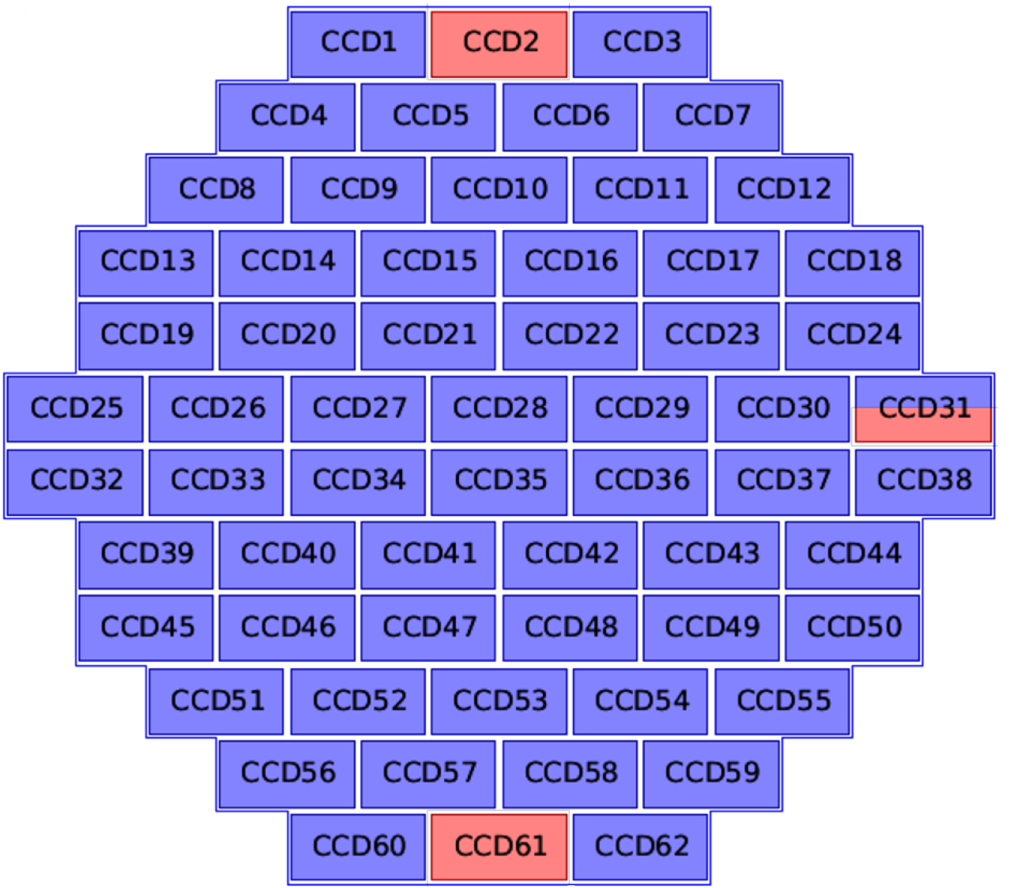
\includegraphics[width=0.6\textwidth]{DECAM_CCD.jpg}
\caption[DECam focal plane]{Focal plane of the Dark Energy Camera (DECam), consisting of 62 CCDs arranged in a hexagonal pattern covering a \SI{3}{\sqdeg} field-of-view. North is displayed at the top and east is on the right. The red sections (CCD 2, CCD 61, and half of CCD 31) were not functional for most of the Year 1 observations used in this catalogue, and data from these regions is not used in this thesis. \textit{Image credit:} \cite{2018ApJS..239...18A}.}
\label{fig:DECAM}
\end{figure} 


Imaging for DES has been obtained with the specially constructed Dark Energy Camera (DECam; \citealt{2015AJ....150..150F}), mounted on the Blanco 4-m telescope at the Cerro Tololo Inter-American Observatory. Containing the latest wide-field imaging technology, DECam has a \SI{3}{\sqdeg} field of view and a 570 megapixel CCD camera, made up of 62 arrays arranged in a hexagonal pattern as per Figure \ref{fig:DECAM}. The camera has a resolution of \SI{0.263}{\arcsec.pix^{-1}}. Observations for DES were conducted using the five main DECam broadband filters $grizY$, of which the transmission curves are plotted in Figure \ref{fig:filters} and wavelength coverage provided in Table \ref{table:effective_wavelengths}. \par



The survey saw first light in September 2012, and observations for the full survey were carried out between August 2013 and January 2019. Over these six years, the \SI{5000}{\sqdeg} wide-field area was covered several times in all five $grizY$ filters to create the footprint shown in Figure \ref{fig:DES_footprint}. In the wide component, each (hexagonal) exposure in the same field was offset by roughly half the focal plane radius, such that objects were observed by different CCDs in each visit. This dithering strategy minimises the effects from inhomogeneities in the DECam apparatus and enhances the photometric calibration. Every year, the exposures collected up to that point are co-added to produce deep imaging (see \citealt{2018ApJS..239...18A} and \citealt{2018PASP..130g4501M} for details), which will reach the final survey depths after the full five years' worth of data have been processed. \par 



\begin{figure}[!pht] 
\centering    
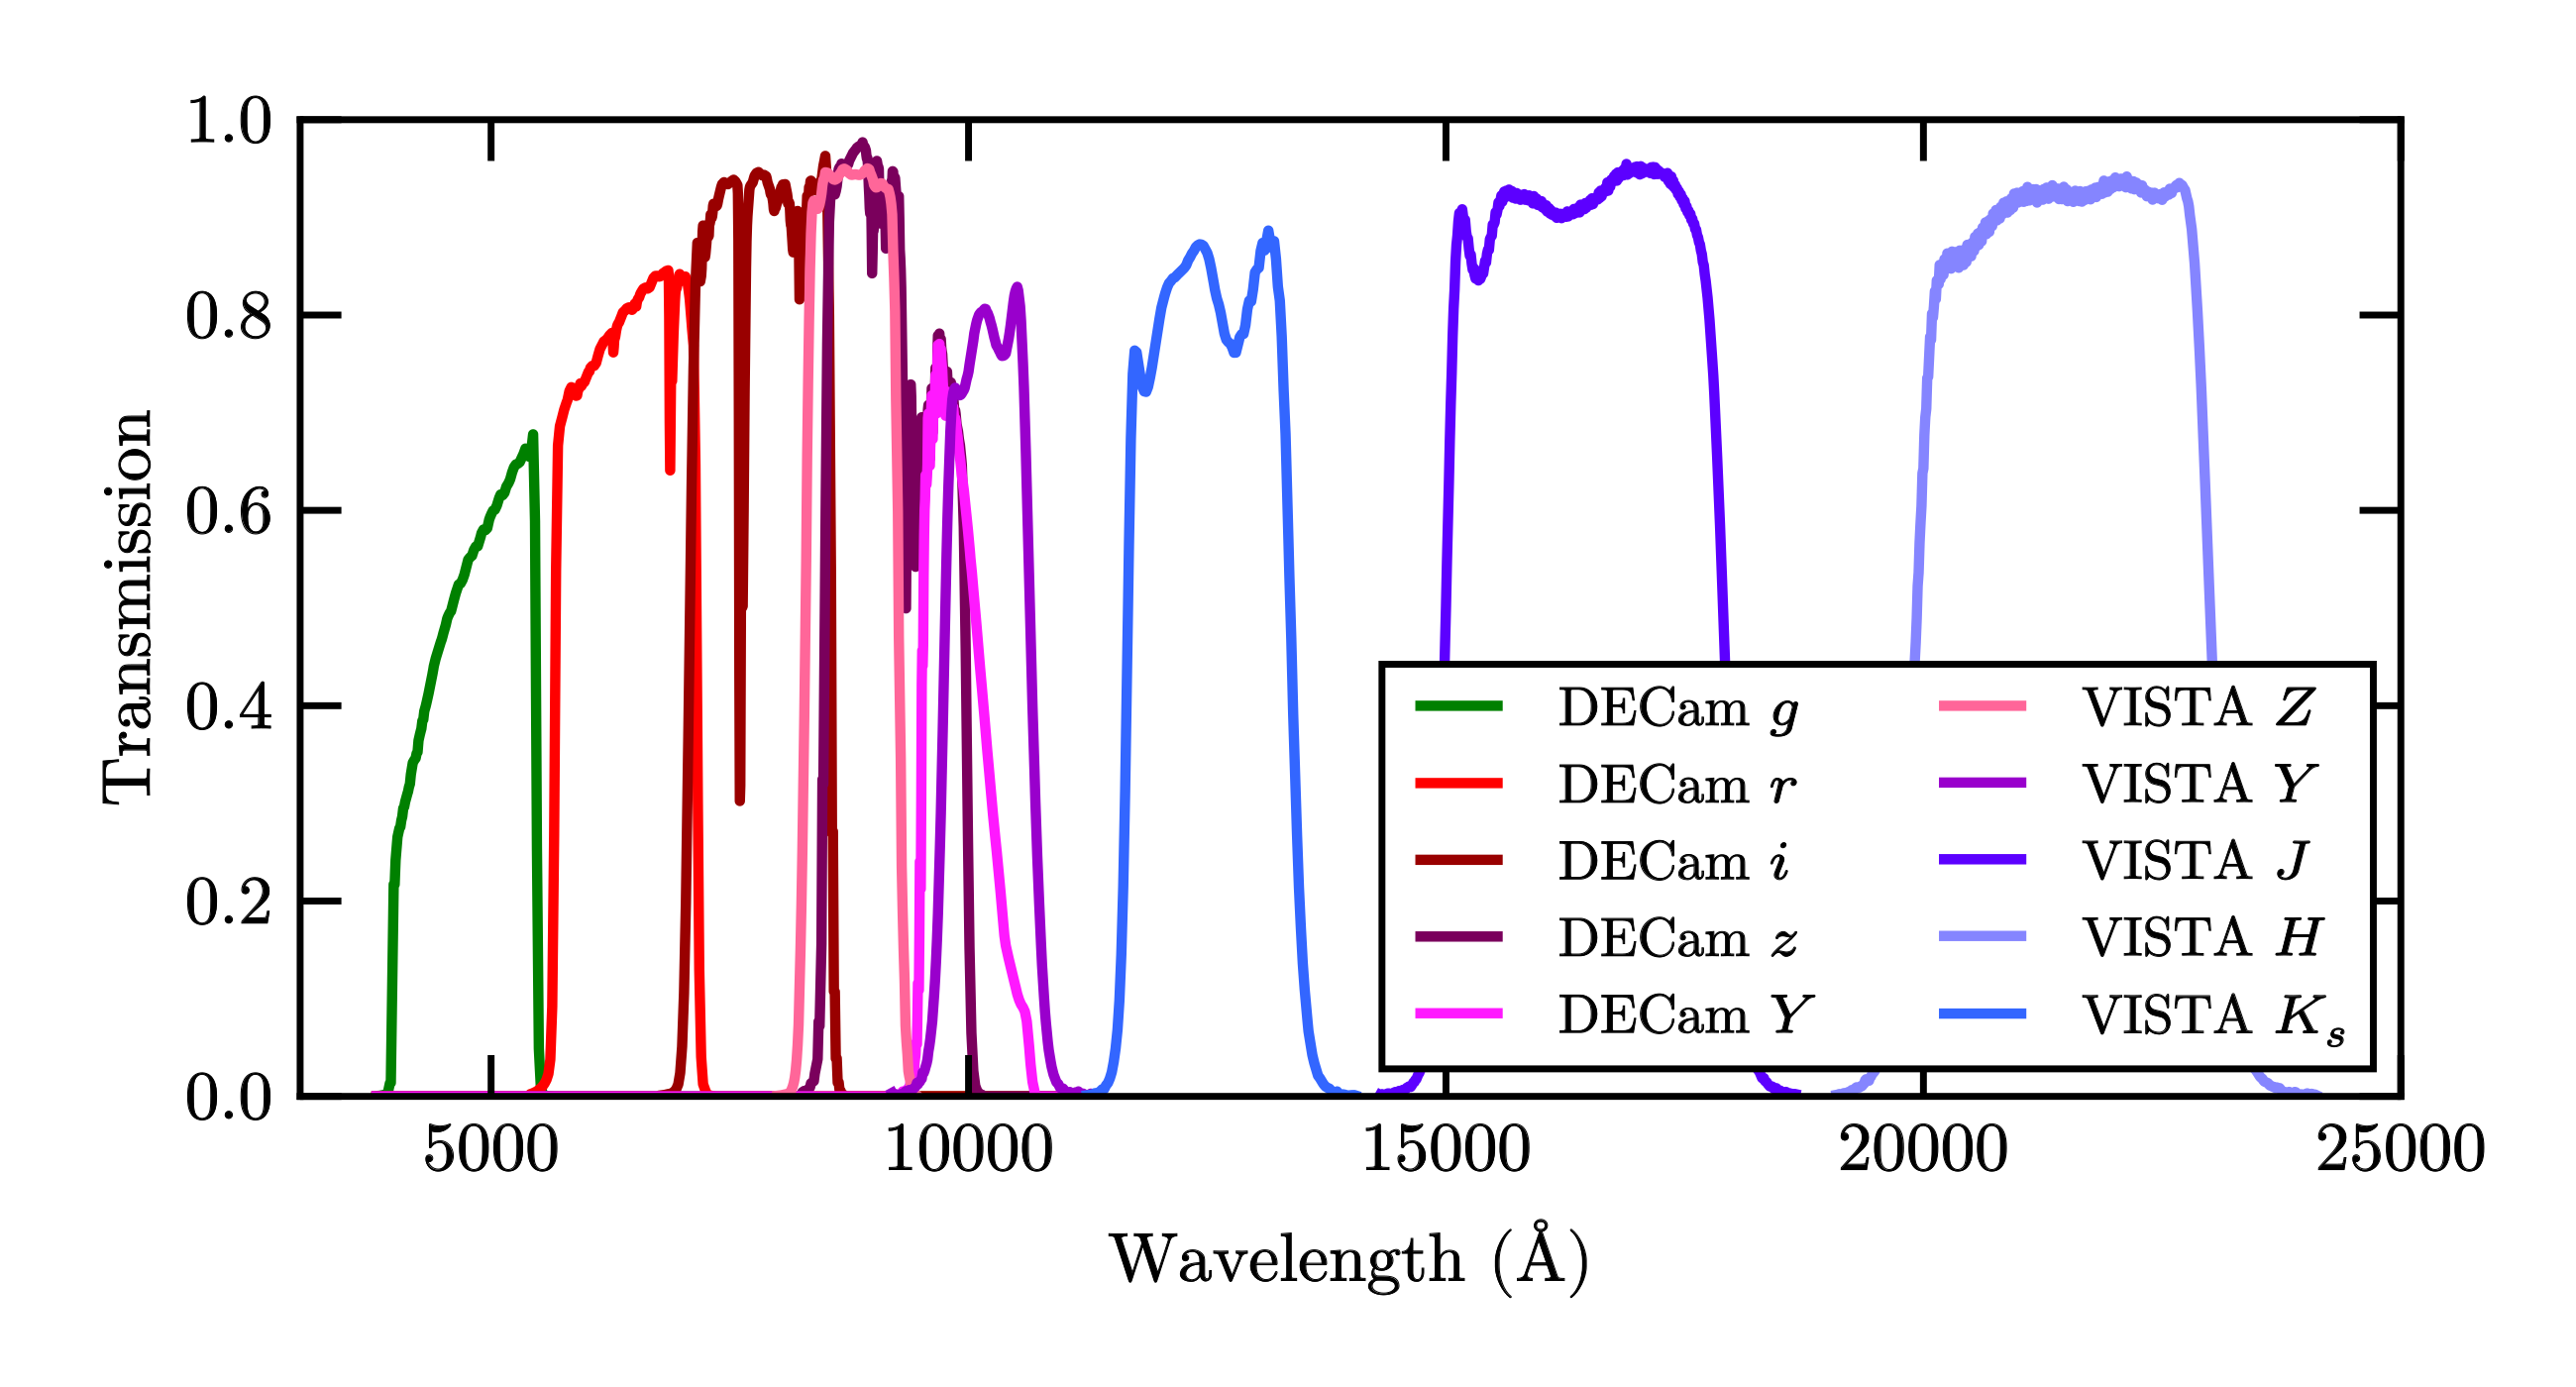
\includegraphics[width=0.95\textwidth]{filters.png}
\caption[DES and VIDEO filter transmission curves]{Transmission curves for the optical to near-infrared filters used in this project from DES (DECam) and VIDEO (VISTA). These plots show the relative total throughput, including the effects of the atmosphere and quantum efficiency of the detector.}
\label{fig:filters}
\end{figure}

\begin{table}[!phb]
\centering
\textsc{Wavelength coverage of filters} \\
\vspace{0.1em}
\footnotesize
\begin{tabular}{lcccclccc}
\toprule\toprule
\multicolumn{4}{c}{\textsc{DECam}} & &  \multicolumn{4}{c}{VISTA}  \\
Filter & $\lambda_{\mathrm{cent}}$ (\si{\angstrom}) & $\lambda_{\mathrm{min}}$ (\si{\angstrom}) & $\lambda_{\mathrm{max}}$ (\si{\angstrom}) & & Filter & $\lambda_{\mathrm{cent}}$ (\si{\angstrom}) & $\lambda_{\mathrm{min}}$ (\si{\angstrom})  & $\lambda_{\mathrm{max}}$ (\si{\angstrom}) \\
\midrule
$g$ & 4730 & 3980 & 5480 & & $Z$ & 8780 & 8285 & 9255 \\ 
$r$ & 6420 & 5680 & 7160 & & $Y$ & 10200 & 9735 & 10665 \\
$i$ & 7840 & 7100 & 8570 & & $J$ & 12520 & 11660 & 13380 \\
$z$ & 9260 & 8500 & 10020 & & $H$ & 16450 & 14995 & 17905 \\
$Y$ & 10090 & 9530 & 10650 & & $K_{s}$ & 21470 & 19925 & 23015 \\
\bottomrule
\end{tabular}
\vspace{1em}
\caption[Wavelength coverage of broadband filters]{The central wavelengths $\lambda_{\mathrm{cent}}$, and left and right edges $\lambda_{\mathrm{min}}$ and $\lambda_{\mathrm{max}}$ for all DECam and VISTA filters used in this thesis. $\lambda_{\mathrm{min}}$ and $\lambda_{\mathrm{max}}$ are defined as the wavelength at which 50\% relative transmission occurs. Each central wavelength is a simple interpolation between $\lambda_{\mathrm{min}}$ and $\lambda_{\mathrm{max}}$.}
\label{table:effective_wavelengths}
\end{table} 




\begin{figure}[htb] 
\centering    
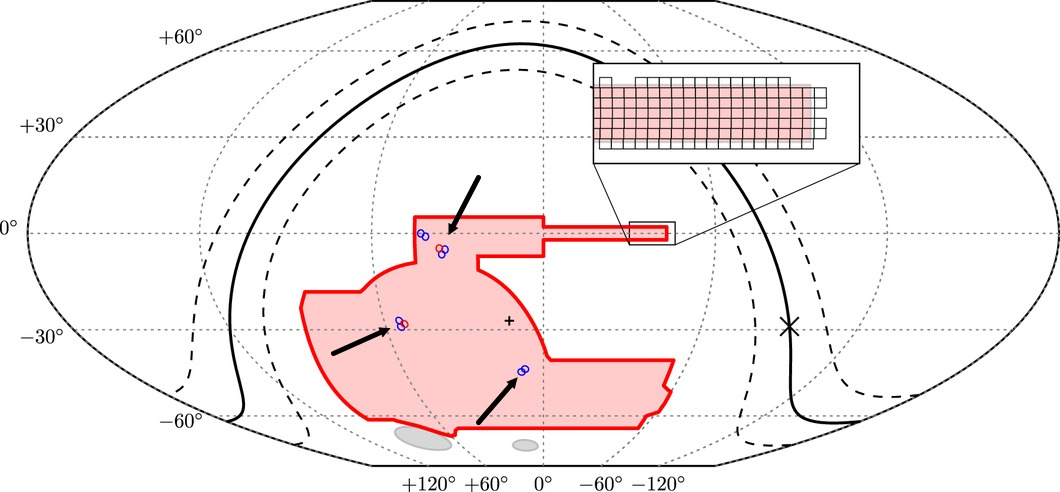
\includegraphics[width=1.0\textwidth]{Chapter2/Figs/DES_footprint_arrows.jpg}
\caption[Map of the DES footprint]{Map of the Dark Energy Survey (DES) area in celestial coordinates. The \SI{5000}{\sqdeg} wide-field survey is shown in red. The eight shallow supernova (SN) fields are displayed as blue circles, and the two deep SN fields are displayed as red circles. The catalogue created in this thesis is based on the eight most southern SN fields, denoted by the black arrows. The other two SN fields around the celestial equator are not included in this work, because they do not overlap with any near-infrared data of a suitable depth. The black line presents the Milky Way plane, and the Galactic center and Galactic pole are marked by a cross ($\times$) and a plus ($+$) respectively. The inlay shows the way the wide-field survey is cut up into co-add tiles by the DESDM processing pipeline. \textit{Image credit:} \cite{2018ApJS..239...18A}}
\label{fig:DES_footprint}
\end{figure}


The time-domain survey has employed a different observing strategy. In this component, the target fields were observed frequently using $griz$ filters only, at regular intervals approximately seven nights apart \citep{2015AJ....150..172K}.  Similarly to the wide-field survey, these exposures are then co-added. These co-added images constitute the so-called DES deep fields, interchangeably referred to as supernova fields. As they contain a substantially higher number of exposures per unit area, these fields reach $\sim\SIrange{1}{2}{\magab}$ deeper in $griz$ compared to the rest of DES. $Y$-band coverage in the supernova fields is provided by the (shallower) wide-field data. In contrast with the main survey, where subsequent exposures in the same field were dithered to achieve maximum data uniformity, each supernova pointing in a given field is the same to within a few arcseconds \citep{2015AJ....150..172K}. While this is useful for supernova science, since it makes it easy to identify if an object has changed in brightness between pointings, an unfortunate side effect of this observing strategy is the presence of chip gaps in the co-added images. These chip gaps originate from the arrangement of the DECam CCDs, which, as demonstrated in Figure \ref{fig:DECAM}, are not perfectly adjacent (see Figures \ref{fig:depth_es1}, \ref{fig:depth_xmm}, and \ref{fig:depth_cdfs} for a visible imprint of these gaps in the data). To compensate for the lack of dithering, the supernova survey used a special photometric calibration strategy, detailed in \cite{2015AJ....150..172K}. \par



The DES deep fields, referred to as the \texttt{DFULL} dataset by the DES collaboration,  form the optical component of the \DESVIDEO catalogue presented in this thesis. To illustrate the positions of the fields, their locations are superimposed on the wide-area DES footprint in Figure \ref{fig:DES_footprint}. It is useful to emphasise that, even though DES has observed a total of ten supernova fields, this thesis includes only eight fields (E1, E2, X1, X2, X3, C1, C2 and C3). The other two (S1 and S2, overlapping the SDSS Stripe 82; \citealt{2007ApJS..172..634A, 2009ApJS..182..543A}) were disregarded due to a lack of available deep near-infrared data. Central coordinates for the eight fields in this thesis are provided in Table \ref{table:fields}. The `E' fields overlap the ELAIS-S1 field \citep{1999MNRAS.305..297G}, the `X' fields overlap the \textit{XMM}–\textit{Newton} Large-Scale Structure field (XMM-LSS; \citealt{2004JCAP...09..011P}), and the `C' fields overlap the \textit{Chandra} Deep Field South (CDF-S; \citealt{2011ApJS..195...10X}). Since each supernova field extends over approximately \SI{3}{\sqdeg} (the field-of-view of a single pointing), the area coverage of the optical data available for this thesis totals around \SI{24}{\sqdeg}. \par





\begin{table}[!htbp]
\centering
\textsc{DES deep (supernova) fields} \\
\vspace{0.1em}
\footnotesize
\begin{tabular}{clccc}
\toprule\toprule
DES name & Field & R.A. (J2000) & DEC (J2000) & Type \\
\midrule
E1 & ELAIS-S1  & 00:31:29.86 & -43:00:34.6 & shallow \\
E2 & ELAIS-S1  & 00:38:00.00 & -43:59:52.8 & shallow \\
X1 & XMM-LSS  & 02:17:54.17 & -04:55:46.2 & shallow \\
X2 & XMM-LSS  & 02:22:39.48 & -06:24:43.6 & shallow \\
X3 & XMM-LSS  & 02:25:48.00 & -04:36:00.0 & deep \\ 
C1 & CDF-S  & 03:37:05.83 & -27:06:41.8 & shallow \\
C2 & CDF-S  & 03:37:05.83 & -29:05:18.2 & shallow \\
C3 & CDF-S  & 03:30:35.62 & -28:06:00.0 & deep \\
\bottomrule
\end{tabular}
\vspace{1em}
\caption[Coordinates of the DES deep fields]{Central coordinates of the eight \SI{3}{\sqdeg} DES deep fields, also referred to as supernova fields. The two so-called deep supernova fields X3 and C3 contain more exposures and are  $\sim\SI{1}{\magab}$  deeper than the shallow fields.}
\label{table:fields}
\end{table}



It is important to point out that this thesis exclusively uses of data from the first year of observations (see \citealt{2014SPIE.9149E..0VD}). This dataset was released internally to the DES collaboration as \texttt{Y1A1} \citep{2018ApJS..235...33D} and is a subset of the data published in the first public data release \texttt{DR1} (which covers all the first three years; \citealt{2018ApJS..239...18A}). The reason for including only the \texttt{Y1A1} data is that at the time the work in this thesis was carried out, data from later years was not yet available due to processing delays. Fortunately, the \DESVIDEO catalogue production pipeline presented in this thesis largely uses automated processes, so it would be straightforward to extend this work to incorporate data from any later releases. \par 




\subsubsection{Data reduction}\label{subsubsection:data_reduction}
After the Year 1 exposures had been taken, the data was processed and combined into deep co-added images. Before this could occur, all DES exposures were required to pass preliminary quality checks on the point spread function (PSF) and signal-to-noise ratio, detailed in  \cite{2018ApJS..235...33D}. The exposures that passed these quality control standards were then processed by the DES data management system (DESDM;  \citealt{2011arXiv1109.6741S, 2012SPIE.8451E..0DM, 2018PASP..130g4501M}), with the aim of producing science ready imaging. The details of this procedure are described at length in \cite{2018ApJS..235...33D} for the \texttt{Y1A1} data used in this thesis. During data processing, the DESDM pipeline removed instrumental signatures from the telescope and DECam setup, and performed masking of artefacts including bright stars, cosmic rays, and fast-moving transients such as satellites and meteors. The DESDM algorithm also created weight images. These weight planes were generated for each individual exposure based on the inverse variance of a flat field image, as this variance captures the Poisson noise and read noise of the instrument. Weight values were then set to zero for all saturated pixels in bright stars, and for masked pixels from artefacts and transients.  \par


The processed exposures then underwent a second round of quality control cuts, intended to blacklist and remove individual CCD images with severe imaging artefacts from phenomena such as scattered light from bright stars, or airplane and meteor trails. For \texttt{Y1A1}, only 1\% of CCD images {were} discarded in this way, and the details of this procedure can once again be found in \cite{2018ApJS..235...33D}. DESDM then produced image co-adds of all approved images, obtained from the weighted average of all overlapping images (using the weight maps described above). The co-addition was performed using \texttt{SWarp} \citep{2002ASPC..281..228B,2010ascl.soft10068B}, which remapped all pixels onto a uniform grid with a pixel scale of \SI{0.263}{\arcsec.pix^{-1}}. This grid was then cut up into co-add tiles of $\num{10 000 x 10 000}$ pixels (covering $\SI[product-units = repeat]{0.73 x 0.73}{deg}$), as illustrated in the inlay of Figure \ref{fig:DES_footprint}. Tiles overlap at the edges by about \SI{1}{\arcmin}, so that for every observed source there exists a tile where it is at least \SI{0.5}{\arcmin} from the edge. One co-added tile was produced for each $grizY$ filter, in addition to a  \texttt{CHI\_MEAN} combination of the $r+i+z$ co-adds intended as a detection image for extracting photometry  \citep{1999AJ....117...68S,2010ascl.soft10068B,2018ApJS..235...33D}. The $g$-band was omitted from this combined image due to the large PSF and noisy sky background in this filter, and the $Y$-band was rejected because of its limited depth and irregular PSF \citep{2018PASP..130g4501M}. In addition to these science co-adds, co-added weight images for all five filters and the combined detection image were produced from the individual exposure weight plane images described above. Conceptually, the idea behind these co-add weight images is to assign a higher weight to pixels with more exposures, and a lower weight in areas where the data is poor. \par 


\subsubsection{Catalogues}\label{subsubsection:des_catalogues}
As part of the data reduction pipeline, DESDM also generated source catalogues from the DES co-adds. The philosophy at the core of this assembly was to create the most inclusive selection of objects, while maintaining low contamination rates \citep{2018ApJS..235...33D}. Such a wide selection of sources suits the aims of this thesis nicely, as the eventual selection of high-redshift objects in Chapter \ref{chapter:high_redshift_candidates} contains its own specific cuts to narrow down the objects. Furthermore, because of the extensive testing that the DES collaboration has applied to the DESDM pipeline, the resulting data products can be trusted to adhere to high quality standards. For these reasons, this thesis has adopted the DESDM catalogues for its optical photometry. \par 

These DESDM catalogues were created with \texttt{SExtractor} (\citealt{1996A&AS..117..393B}), according to a procedure detailed in  \cite{2018ApJS..235...33D}. Objects were detected in the aforementioned combined $r+i+z$ image, and photometry was extracted in each $grizY$ filter based on the detected positions in the combined image.  This technique of using a different image for detection and source extraction is commonly referred to as `forced photometry', and will be revisited in  Section \ref{section:forced_photometry}.  \par


Despite the great diligence with which the DES collaboration has optimised photometric calibration, there nevertheless exist some colour non-uniformities in the DESDM images and catalogues used as the optical backbone for this thesis \citep{2018ApJS..235...33D}. These discrepancies are due to position-dependent variations in the photometric calibration, together with varying levels of Galactic reddening over the survey footprint. The DES collaboration has resolved these issues by determining magnitude corrections, derived via the so-called  stellar locus regression (SLR) method \citep{2004AN....325..583I, 2009AJ....138..110H, 2012ApJ...757...83D, 2014MNRAS.439...28K}. Using a code by \cite{2014MNRAS.439...28K}, \cite{2018ApJS..235...33D} employed this technique to calibrate the proper photometric zero-points from the particular shape of the stellar locus in colour-colour space. Using the DES colours of star samples in $\sim\SI{0.1}{\sqdeg}$ segments, the appropriate SLR correction was determined empirically for each segment of the total footprint. For the data in this thesis, these corrections are later applied by the author at the catalogue level, as will be described in Section \ref{subsection:catalog_production}.  \par




\subsubsection{Data quality}\label{subsubsection:data_quality}
In order to provide an overview of the quality of the optical data in this thesis, this section will outline several important properties of the DES deep field data, specifically the seeing, depths, and weight flags. \par   


%Having described the DES data collection and reduction procedures, the discourse will now turn to the quality of the resulting data products. This discussion will describe the seeing, depth, and weight flags in the DES deep fields, which are


%Having described the data collection and reduction procedures, the discussion will now evaluate the data quality of the resulting data products. 
%\paragraph{} {\color{red} The discussion will now turn to an analysis of the data quality in the images and DESDM catalogues. }

%In order to provide an overview of the quality of the optical data in this thesis, the following section investigates several important properties of the DES deep field data. 

%Due to their importance to the rest of this project these quantities include the seeing, depth and weight flags.  


\paragraph{Seeing}  The DES observing protocol dictated that the supernova fields had to be observed (1) when the seeing was above \SI{1.1}{\arcsec} and thus deemed inadequate for the precision cosmology requirements of the wide-field survey, or (2) when a particular supernova field had not been observed for 7 days. As a result, the seeing in the DES deep fields varies considerably. To eliminate any data with a PSF that is too poor for many scientific applications, the preliminary quality checks described in Section \ref{subsubsection:data_reduction} imposed a quality cut of FWHM < \SI{2}{\arcsec} on any exposures that were included in the co-adds. All in all, these various constraints on the seeing have resulted in an average PSF width of $\sim \SI{1.0}{\arcsec}$ in the DES deep fields \citep{2015AJ....150..172K}. 


\paragraph{Depths} The observing strategy described in Section \ref{subsubsection:data_collection} created inhomogeneous coverage over the DES footprint. Because each field contains regions with different numbers of exposures, the survey depths are non-uniform both across and inside tiles. The heterogeneous nature of the data is increased further by the effect of dead CCDs, chips gaps, and masked objects (e.g. stars and satellite or airplane streaks). With this in mind, the DES collaboration has provided a rigorous analysis of the coverage and depth variation, by creating depth maps that chart the limiting magnitude as a function of sky position. The paper by \cite{2018ApJS..235...33D} describes the creation of these maps in detail. In essence, their approach used the \texttt{mangle} code \citep{2004MNRAS.349..115H,2008MNRAS.387.1391S} to capture the DES survey coverage, firstly masking out bad regions and dividing the DES data into segments. For each segment, the $10\sigma$ limiting magnitude in a \SI{1.95}{\arcsec} aperture in a given filter (i.e. $m_{10\sigma}$) was then calculated based on the \texttt{mangle} co-add weight maps (created from the DESDM weight images\footnote{To be precise, \texttt{mangle} produced its own co-add weight maps from the individual exposure weights rather than the final co-add weight maps.} mentioned in Section \ref{subsubsection:data_reduction}). These calculations used the following equation:

\begin{equation}
m_{10\sigma} = m_{\mathrm{zp}} - 2.5 \log{10 \sqrt{\pi \frac{(D/2)^2}{\omega^2_{\mathrm{pix}}} \frac{1}{w_{\mathrm{tot}}}}},
\end{equation}

\noindent where $m_{\mathrm{zp}}=30$ is the photometric zero-point for the DES tiles, $D=\SI{1.95}{\arcsec}$ is the aperture diameter, $\omega_{pix} = \SI{0.263}{\arcsec.pix^{-1}}$ is the pixel scale and $w_{tot}$ is the total co-added weight in a particular \texttt{mangle} segment. The resulting map of $10 \sigma$ limiting magnitudes was then pixelised and stored as a \texttt{HEALpix} map, which was distributed to the DES collaboration.   \par


The depths from this map are later added to the \DESVIDEO catalogue by the author, together with depths for other values of $\sigma$ (as will be detailed in Section \ref{subsection:catalog_production}). The procedure used to calculate these other depths is as follows. Following \cite{2015arXiv150900870R}, the $10\sigma$ limiting magnitudes in the \texttt{HEALpix} map are firstly converted to other depths via the effective exposure time $t_{\mathrm{eff}}$, which for each filter can be parameterised as a function of limiting magnitude:

\begin{equation}
t_{\mathrm{eff}} = \exp{ \left( a + b \ (m_{10\sigma}-21.0) \right) }.\label{eqn:t_eff}
\end{equation}

\noindent In this formalism $m_{10\sigma}$ is the $10\sigma$ limiting magnitude, 21.0 is a convenient pivot point, and $a$ and $b$ are parameters that were provided by the DES collaboration (obtained by fitting to the DES data). The effective exposure time is related to the flux noise $F_{\mathrm{noise}}$ via

\begin{equation}
F_{\mathrm{noise}} = \frac{F^2_{10\sigma} \ t_{\mathrm{eff}}}{10^2} - F_{10\sigma},\label{eqn:F_noise}
\end{equation}

\noindent and the $10\sigma$ limiting flux $F_{10\sigma}$ required to compute this flux noise can be obtained  straightforwardly from the aforementioned $10\sigma$ limiting magnitudes: 

\begin{equation}
F_{10\sigma} = 10^{(m_{10\sigma}-m_{\mathrm{zp}})/2.5}.\label{eqn:f_10}
\end{equation}

\noindent Here $m_{\mathrm{zp}}=30$ once more represents the photometric zero-point\footnote{The DES collaboration wiki pages mention that this zeropoint ought to be 22.5. However, the author believes that this was likely a mistake, since the paper by \cite{2018ApJS..235...33D} clearly states that the tile zero-point value used in the $m_{\mathrm{lim},10\sigma}$ computations is 30.0. The reason why the wiki pages list a value of 22.5 is likely that the equations on these pages were copied directly from \cite{2015arXiv150900870R}. That paper was written based on SDSS data, where the zero-point is indeed 22.5. The author has calculated the difference in depths between either of these zero-points, and fortunately determined that they were of the order of $\sim \SI{0.02}{\mag}$, so even if the assumption of $m_{\mathrm{zp}}=30.0$ in this thesis is in fact not correct, the effect of this choice is very small.}. Combining Equations \ref{eqn:t_eff}, \ref{eqn:F_noise}, and \ref{eqn:f_10} yields $F_{\mathrm{noise}}$, which can then be translated into limiting fluxes $F_{N\sigma}$ for other values of $\sigma$ denoted by $N$ (in this formalism $N=5$ yields $5\sigma$ depths): 

\begin{equation}
F_{N\sigma}= \frac{N^2+\sqrt{(N^2)^2+4t_{\mathrm{eff}}N^2F_{\mathrm{noise}}}}{2t_{\mathrm{eff}}}.
\end{equation}

\noindent Finally, these limiting fluxes are converted back to magnitudes to obtain the final limiting magnitude $m_{N\sigma}$ for an arbitrary number $N$:

\begin{equation}
m_{N\sigma} = m_{\mathrm{zp}} -2.5\log{F_{N\sigma}}  \label{eqn:m_n}  .
\end{equation}

\noindent Via this method, $7.5\sigma$, $5\sigma$, $3\sigma$, and $1\sigma$ depths can be computed for every DES filter. Section \ref{subsection:catalog_production} will describe how these values are eventually added to the \DESVIDEO catalogue, so that the final data product contains $m_{10\sigma}$, $m_{7.5\sigma}$, $m_{5\sigma}$, $m_{3\sigma}$, $m_{2\sigma}$ and $m_{1\sigma}$ limiting magnitudes in the $grizY$-bands for each object. \par 


\begin{figure}[!ph] 
\centering    
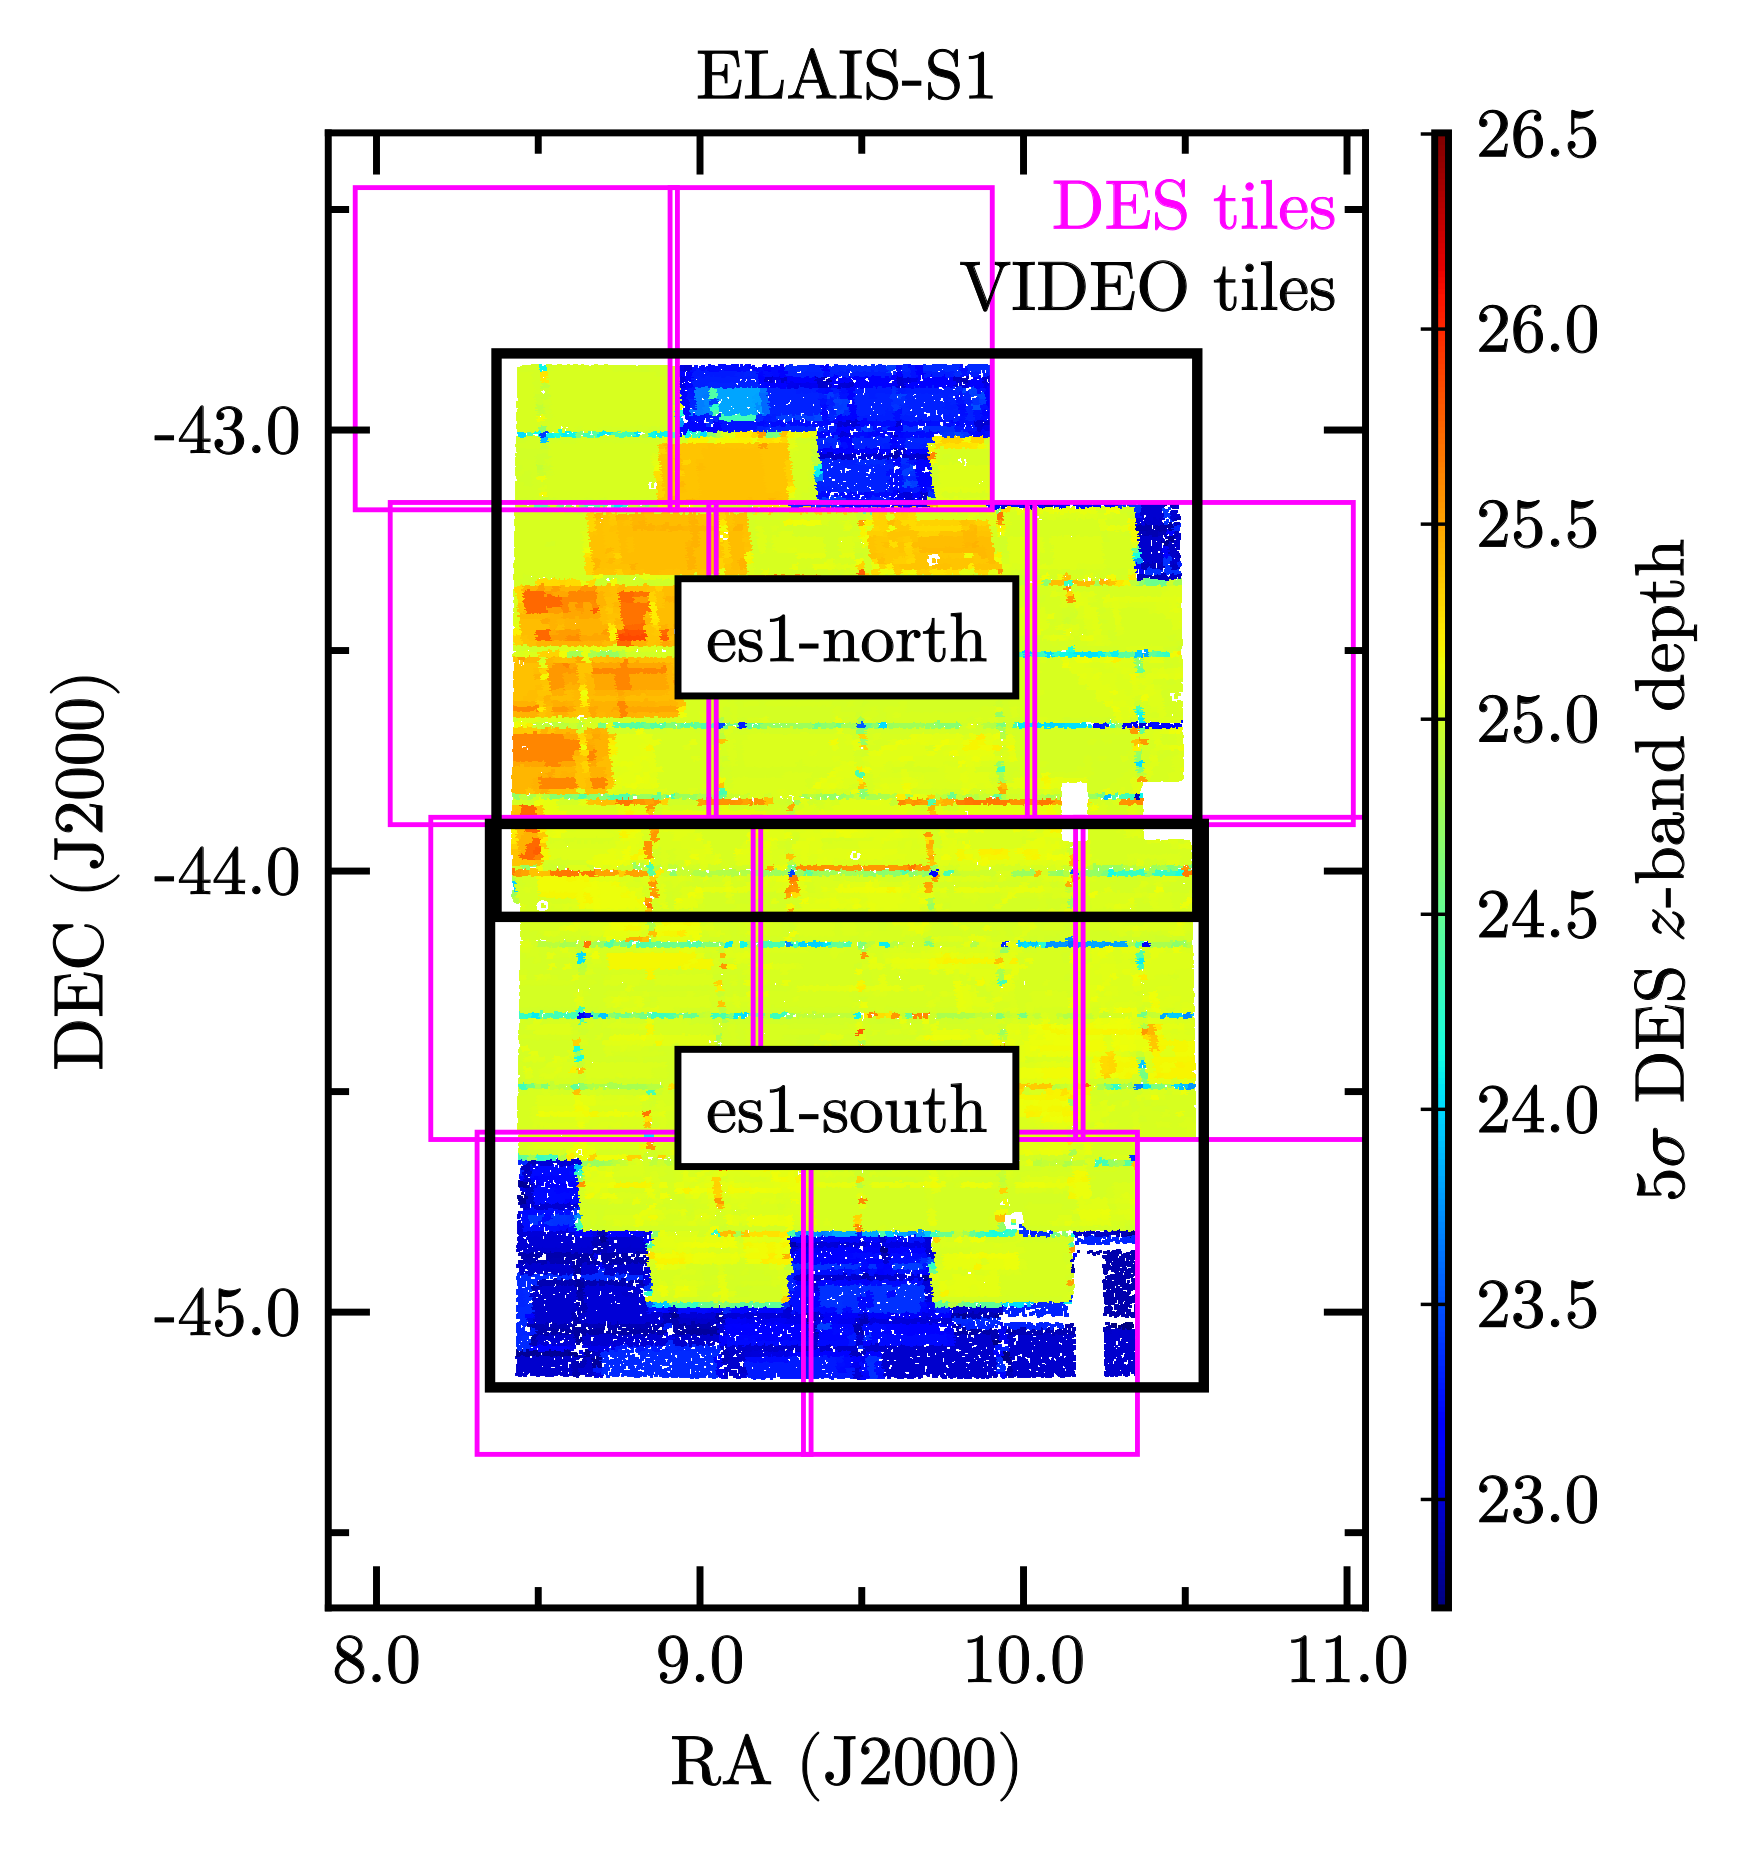
\includegraphics[width=0.618\textwidth]{field_outline_es1.png}
\caption[Depths in the ELAIS-S1 field]{$z$-band $5\sigma$ limiting magnitudes in \SI{1.95}{\arcsec} apertures for the DES data that overlaps the VIDEO footprint in the ELAIS-S1 field. These depths have been derived from the $10\sigma$ depth maps provided by the DES collaboration as detailed in the text. The DES collaboration has included the SLR corrections described in Section \ref{subsubsection:des_catalogues} in their $10\sigma$ depth estimates. The magenta squares show the edges of the DES co-add tiles. VIDEO tiles are outlined in black.}
\label{fig:depth_es1}
\end{figure}

\begin{figure}[!htb] 
\centering    
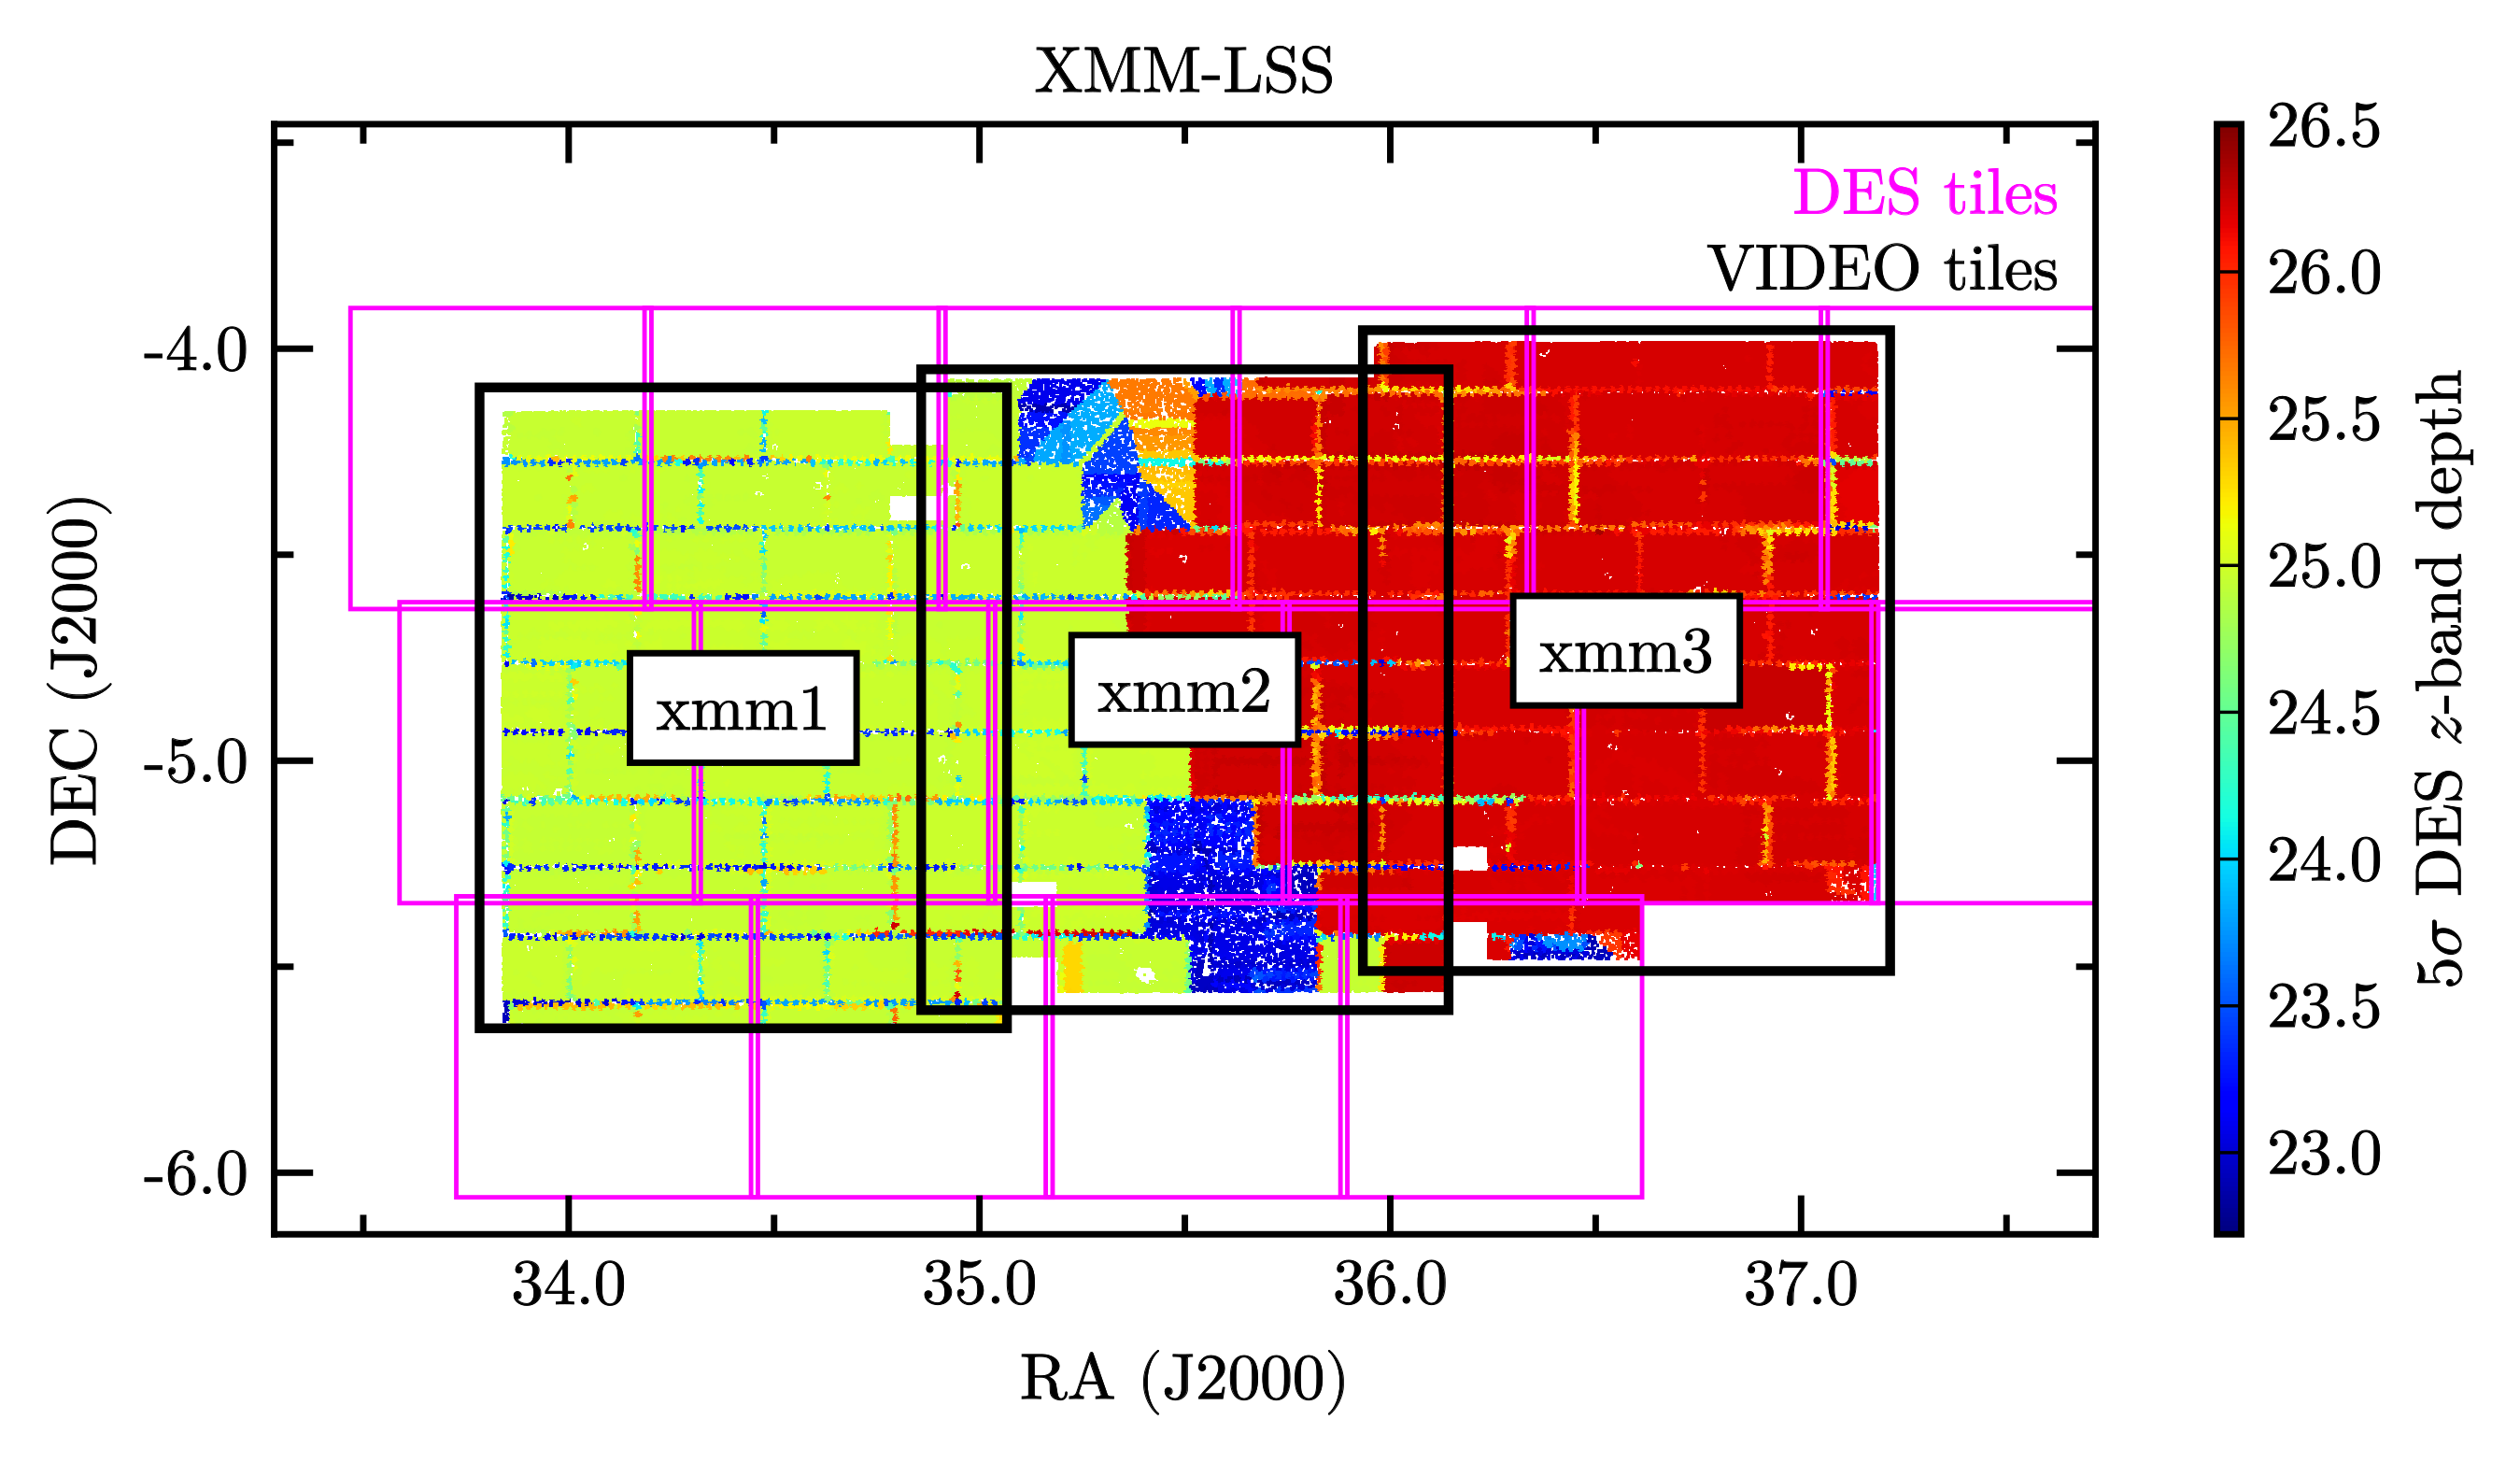
\includegraphics[width=0.95\textwidth]{field_outline_xmm.png}
\caption[Depths in the XMM-LSS field]{$z$-band $5\sigma$ limiting magnitudes in \SI{1.95}{\arcsec} apertures for the XMM-LSS field. The image description is otherwise identical to that of Figure \ref{fig:depth_es1}. The red regions correspond to the deep supernova field X3.}
\label{fig:depth_xmm}
\end{figure}

\begin{figure}[!htb] 
\centering    
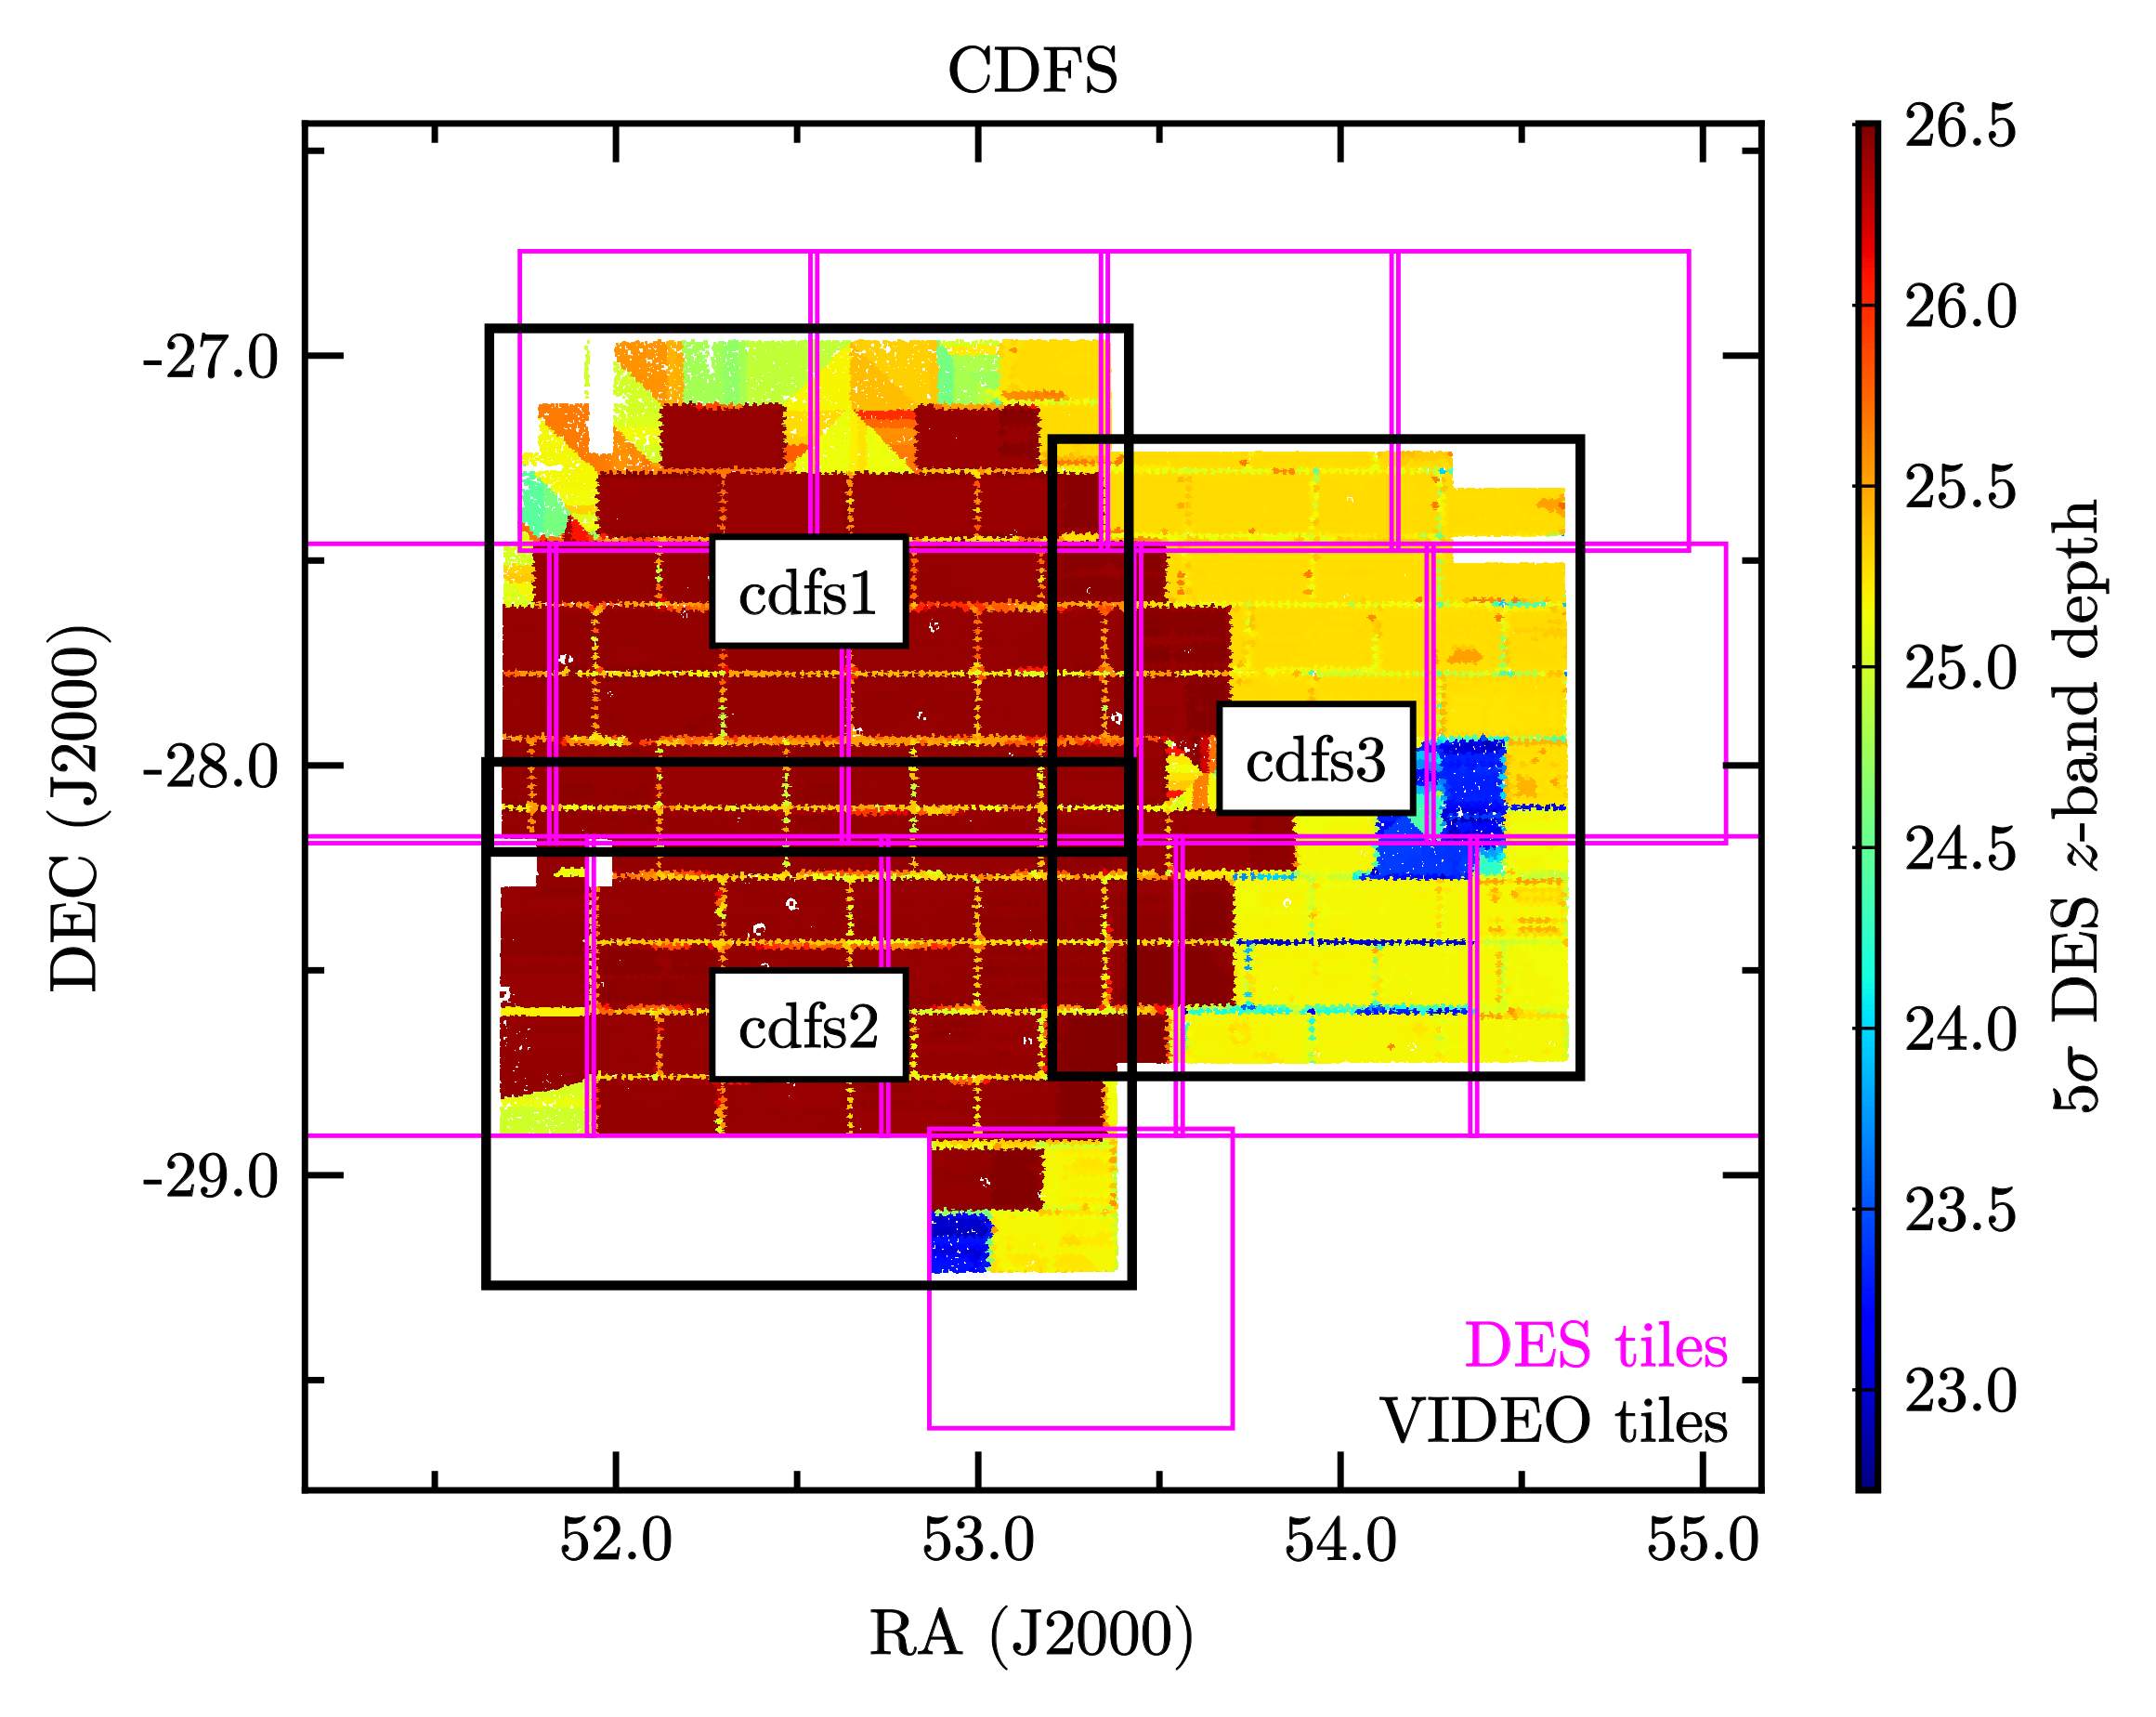
\includegraphics[width=0.825\textwidth]{field_outline_cdfs.png}
\caption[Depths in the CDF-S field]{$z$-band $5\sigma$ limiting magnitudes in \SI{1.95}{\arcsec} apertures for the CDF-S field. The image description is otherwise identical to that of Figure \ref{fig:depth_es1}. The red regions correspond to the deep supernova field C3.}
\label{fig:depth_cdfs}
\end{figure}


To visualise the depths in the eventual \DESVIDEO catalogue, the $z$-band $5\sigma$ depth maps (obtained from the $10\sigma$ DES maps as described above) are plotted in Figures \ref{fig:depth_es1}, \ref{fig:depth_xmm} and \ref{fig:depth_cdfs} for the ELAIS-S1, XMM-LSS, and CDF-S fields respectively. It must be noted that these maps contain only the DES data included in the combined \DESVIDEO catalogue, and that they thus display only regions that overlap the VIDEO survey. The plots clearly show the heterogenous nature of the DES data, as well as the imprint of the hexagonal DECam CCD array and chip gaps in between CCDs. They also illustrate the varying coverage in the DES supernova fields, clearly demonstrating the higher depths in the deepest regions X3 and C3 (see Table \ref{table:fields}). An overview of the depth variation in all DES filters is given in Table \ref{table:actual_des}, which shows the minimum, maximum and median values of the $5\sigma$ depths for the full $grizY$ filterset. \par


\begin{table}[!bt]
\centering
\textsc{$5\sigma$ limiting magnitudes in the DES deep fields} \\
\vspace{0.1em}
\footnotesize
\begin{tabular}{lcc}
\toprule\toprule
Filter & $5\sigma$ depth range (\si{\magab}) & Median $5\sigma$ depth (\si{\magab})  \\
\midrule
$g$ & 24.2 - 26.9 & 25.9 \\
$r$ & 23.8 - 26.9 & 25.6 \\
$i$ & 23.3 - 26.6 & 25.4 \\
$z$ & 22.7 - 26.5 & 25.2 \\
$Y$ & 21.2 - 23.5 & 23.1 \\
\bottomrule
\end{tabular}
\vspace{1em}
\caption[Range of depths in the DES deep fields]{Minimum, maximum, and median (averaged over area) values of the $5\sigma$ limiting magnitudes in \SI{1.95}{\arcsec} apertures, for the DES deep field data overlapping the VIDEO footprint. Values were obtained from the $5\sigma$ depth maps derived as per the text, based on the $10\sigma$ limiting magnitude maps provided by the DES collaboration. The significantly lower $Y$-band depths are explained by the fact that $Y$-band coverage is provided by the wide-area survey, which is considerably shallower. 
}
\label{table:actual_des}
\end{table}


To measure the effective area available for specific science goals, it is useful to consider the total \DESVIDEO area that is available to a given depth. This quantity is explored in Figure \ref{fig:area_depth}, which for each of the $grizY$ filters shows the relationship between a given $5\sigma$ limiting magnitude and the total area with that limiting magnitude or higher. Out of the total combined footprint of \SI{12.1}{\sqdeg}, the largest part ($\approx\SI{11}{\sqdeg}$ in $griz$) comes from the supernova fields. The remaining coverage ($\approx\SI{1}{\sqdeg}$ of the $griz$-bands and all of the $Y$-band) is from the wide-field survey. The effect of the shallow and deep supernova fields (see Table \ref{table:fields}) can be seen in the two `steps' of the $griz$ distributions. In the $z$-band, for instance, there is \SI{10.8}{\sqdeg} available to $5\sigma$ depths of $z_{5\sigma}=24.9$, originating from all eight supernova fields (deep and shallow). A sub-area of \SI{4.3}{\sqdeg} extends even further to $z_{5\sigma}=26.2$; this data comes from the deep supernova fields X3 and C3. \par

\begin{figure}[!htb] 
\centering    
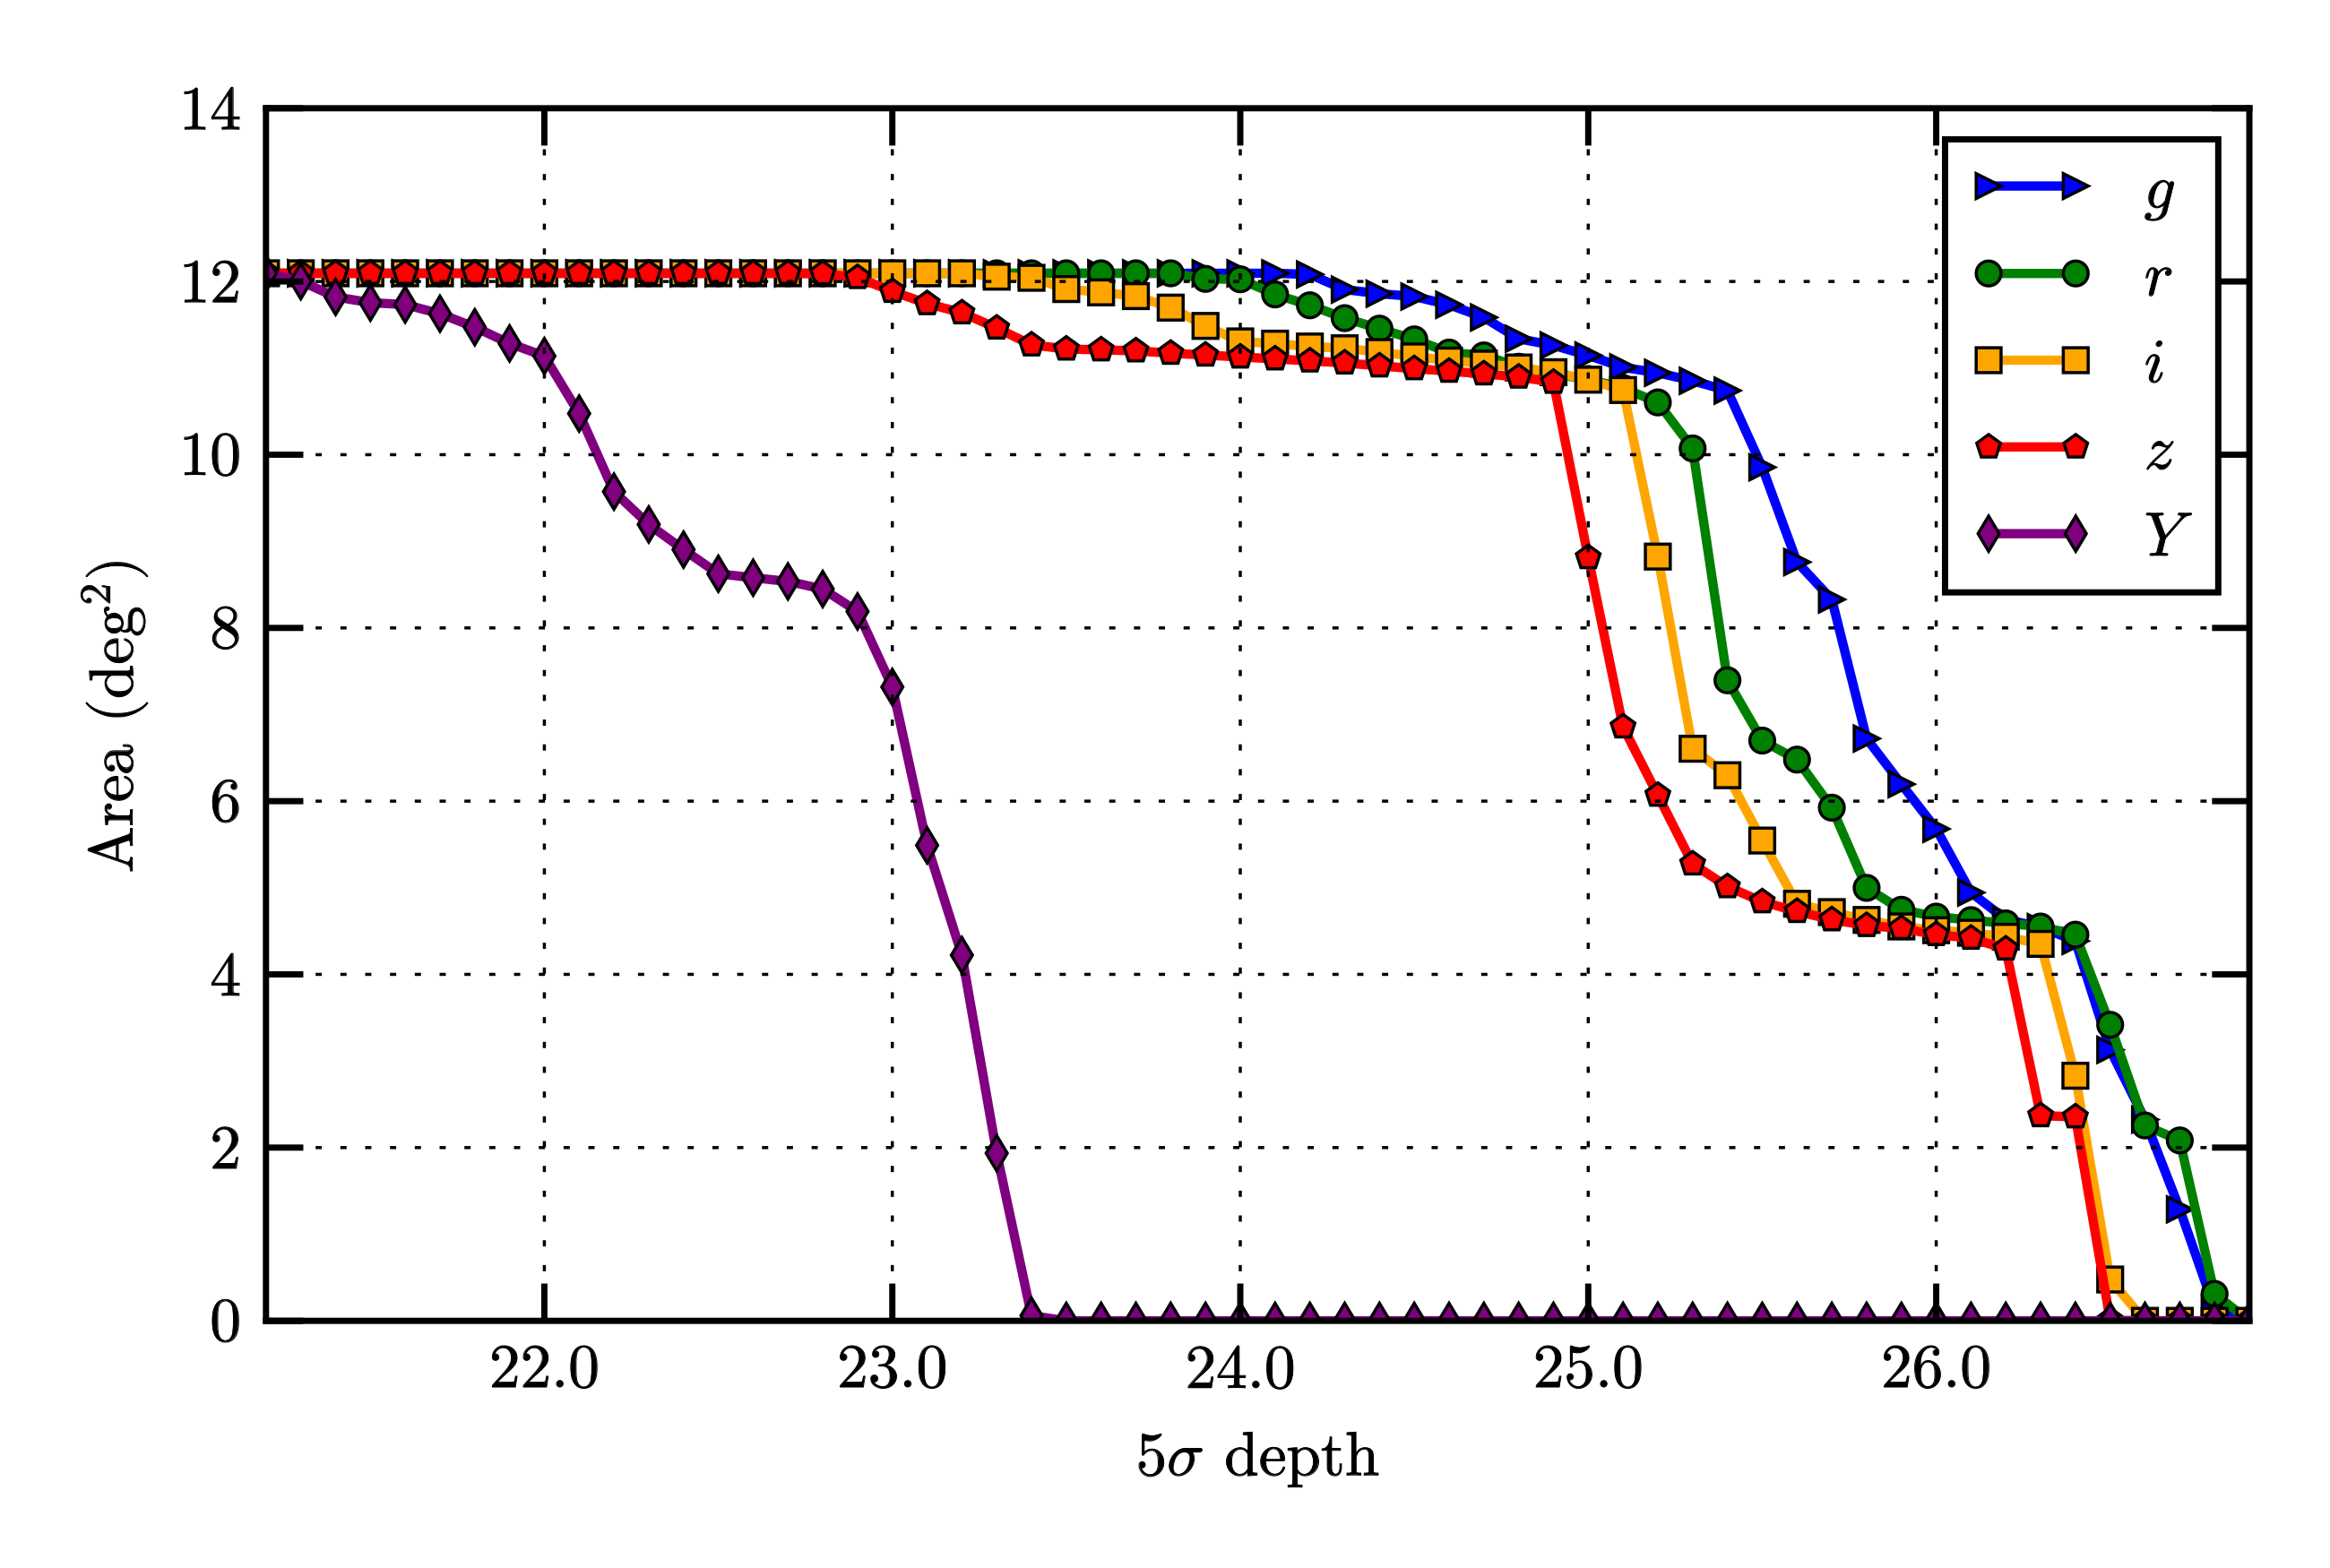
\includegraphics[width=0.95\textwidth]{area_depth_plot_5sig.png}
\caption[Area as a function of \texorpdfstring{$5\sigma$}{} depth for the total survey footprint]{The area available to a given $5\sigma$ depth as a function of that depth, for the catalogue produced in this thesis. The plotted area contains only DES data overlapping VIDEO. Area-depth functions are shown for all five DES filters.}
\label{fig:area_depth}
\end{figure}

Although the \SI{10.8}{\sqdeg} area with $z_{5\sigma}=24.9$ that remains after considering VIDEO overlap is much less than the total $\sim\SI{24}{\sqdeg}$ of DES data available, a comparison with similar surveys in Table \ref{table:ground_small_survey} demonstrates that it is still among the largest footprints to these depths. What is more, the $z_{5\sigma}=26.2$ limiting magnitudes in the deepest \SI{4.3}{\sqdeg} regions are comparable to those of the CFHTLS deep fields, which currently comprise the deepest optical imaging over $\sim \SI{4}{\sqdeg}$. The area-depth coverage of the catalogue in this thesis turns out to be even more significant when also considering the VIDEO limiting magnitudes, because together the \DESVIDEO combined footprint covers the largest area among existing optical+near-IR datasets with comparable near-infrared depths.  This point will be revisited in Section \ref{subsubsection:data_quality_video}, where the VIDEO depths will be introduced and discussed.  \par
%CHANGE THIS MAKE IT NICER 



\paragraph{Weight flags}
To identify sources with questionable photometry, the DESDM catalogues contain a \texttt{FLAGS\_WEIGHT} column that indicates when \texttt{SExtractor} extracted photometry on an object with low weights (as determined from the $r+i+z$ co-add weight maps). \texttt{SExtractor} assigns a \texttt{FLAGS\_WEIGHT} value of 1 to objects which overlap pixels in the weight map below a threshold value \texttt{WEIGHT\_THRESH}, and a value of 2 to objects that are adjacent to pixels below the \texttt{WEIGHT\_THRESH} value\footnote{More specifically, when the isophotal footprint assigned to an object by \texttt{SExtractor} overlaps or is adjacent to pixels which fall below this threshold in the detection image weight map.}. All other, unflagged sources are allocated a \texttt{FLAGS\_WEIGHT} value of 0. The DESDM pipeline used a \texttt{WEIGHT\_THRESH} threshold of 0 \citep{2018PASP..130g4501M}, which means in practice that objects with non-zero weight flags overlap or touch regions that were masked out by DESDM. As discussed in Section \ref{subsubsection:data_reduction}, these masked out regions belong to bad pixels or artefacts, for instance from faulty CCDs, chip gaps, saturated parts of bright stars, cosmic rays, and satellite or meteor trails (see \citealt{2018ApJS..235...33D} and \citealt{2018PASP..130g4501M} for the specific details of the masking algorithm). In this thesis, the weight flags are later used to filter out artefacts and objects with unreliable photometry, during the computation of \DESVIDEO photometric redshifts and the assembly of a high-redshift galaxy sample (described in Sections \ref{subsection:photoz_computation_method} and \ref{subsubsection:weight_flag_cut} respectively). \par







%********************************** %Second Section  **************************************
\subsection{The Vista Extragalactic Deep Observations Survey (VIDEO)}\label{section:video}
\subsubsection{Overview}\label{subsubsection:video_overview}
%The importance of NIR data lies in two points.
The VISTA Extragalactic Deep Observations  survey (VIDEO; \citealt{2013MNRAS.428.1281J}) is a near-infrared survey conducted with the Visible and Infrared Survey Telescope for Astronomy (VISTA). Its scientific aims are to study the evolution of galaxies, clusters, and structures as a function of their environment over the cosmic epoch $0<z<4$, and to trace AGN and the most massive galaxies out into the era of reionisation. To this end, VIDEO covers \SI{12}{\sqdeg} in five near-infrared filters ($ZYJHK_{s}$). Imaging over these wavelengths is crucial to both science goals. Firstly, near-IR data is required for the proposed $z<4$ galaxy evolution studies, because above $z>1$ the bulk of the luminosity output required for stellar mass estimates is emitted in these wavebands. Secondly, when approaching the epoch of reionisation at $z\sim6$, the light output of galaxies is almost entirely redshifted into the near-infrared. The VIDEO science goals also require deep imaging over a large area. Previous near-infrared studies have been either too shallow for high-redshift studies (e.g. VIKING, \citealt{2013Msngr.154...32E}; UKIDSS-LAS, \citealt{2007MNRAS.379.1599L}; VHS, \citealt{2013Msngr.154...35M}), or covered too small areas for statistical studies of large-scale environments and for finding uncommon objects such as massive galaxies and AGN (e.g. CANDELS, see Table \ref{table:space_small_survey}; UltraVISTA, see Table \ref{table:ground_small_survey}).  The VIDEO survey bridges this gap, utilizing the state-of-the-art rapid imaging technology on the VISTA telescope that has made it possible to efficiently probe large cosmological volumes. Its combination of area and depth makes VIDEO an ideal candidate to combine with DES optical imaging, creating a dataset excellently suited to the photometric redshift research and high-redshift galaxy search in this thesis. \par

\subsubsection{Data collection}\label{subsubsection:data_collection_video}
VIDEO observations have been conducted with the VISTA Infrared Camera (VIRCAM; \citealt{2006SPIE.6269E..0XD}) on the 4m VISTA telescope \citep{2004Msngr.117...27E, 2015A&A...575A..25S} at the La Silla Paranal observatory. VIRCAM is the world's largest near-IR camera, made up of 16 \num{2048 x 2048} HgCdTe detector arrays totalling 67 megapixel, with a mean pixel scale of \SI{0.339}{\arcsec.pix^{-1}}. The detectors are spaced out over a \SI{1.65}{deg} diameter focal plane, with gaps of 0.9 and 0.425 of a detector along the x- and y-axes respectively,  as illustrated by Figure \ref{fig:VIRCAM}. Excluding these gaps, the 16 detectors cover an effective \SI{0.6}{\sqdeg} field-of-view. The five $ZYJHK_{s}$ broadband VIRCAM filters used for VIDEO are plotted in Figure \ref{fig:filters}, with detailed wavelength coverage specified in Table \ref{table:effective_wavelengths}. \par

\begin{figure}[tbp] 
\centering    
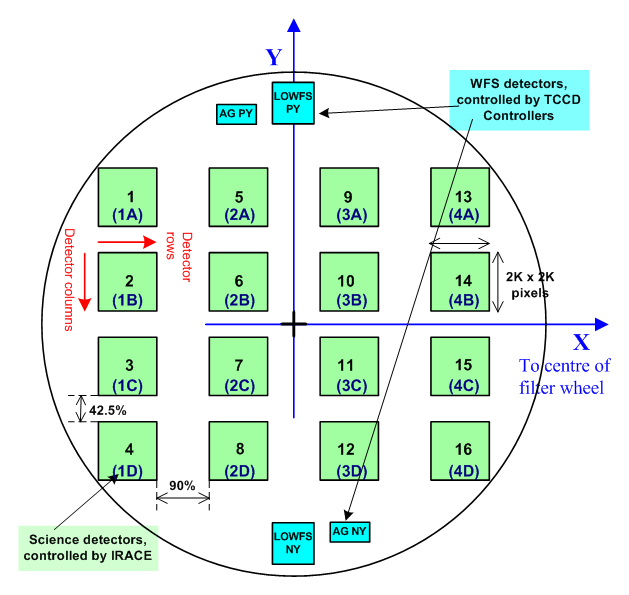
\includegraphics[width=0.75\textwidth]{VIRCAM_detail.png}
\caption[VIRCAM focal plane]{Focal plane of the VISTA Infrared Camera (VIRCAM), made up of 16 HgCdTe detectors. The detectors are spaced out with gaps of 0.9 and 0.425 of a detector in the x- and y-direction respectively. The diameter of the focal plane spans 1.65 deg, and the total effective area covered by all 16 detectors (excluding gaps) is \SI{0.6}{\sqdeg}.  \textit{Image credit:} VISTA ({\color{blue} www.vista.ac.uk})}
\label{fig:VIRCAM}
\end{figure}


Observations commenced in October 2009 and finished in September 2018. Throughout these nine years, imaging was collected using an observing strategy detailed in \cite{2013MNRAS.428.1281J}, which will be now be summarised  briefly. The VIDEO protocol was designed to deal with well-known challenges for near-infrared astronomy, concerning the brightness and variability of the sky background in this wavelength regime (particularly in the $H$- and $K_{s}$-bands). To overcome these issues, individual exposures were split up into small time chunks. Each pointing was observed NDIT times, with a detector integration time DIT (between 10 and 50 seconds depending on the filter), resulting in a total exposure time of $\mathrm{NDIT} \times \mathrm{DIT}$. The telescope was then `jittered' randomly by a small offset of $\lesssim\SI{20}{\arcsec}$, and the $\mathrm{NDIT} \times \mathrm{DIT}$ sequence was repeated at the offset position. This jittering minimises the effect of  both sky fluctuations and detector artefacts such as bad pixels. The totality of $\mathrm{NDIT} \times \mathrm{DIT}$ (jittered) exposures in a given position is called a `paw-print' in VIDEO jargon. Due to the aforementioned gaps between VIRCAM  detectors, these paw-prints do not fill a contiguous area. To cover a full tile, the telescope was moved in a sequence of six offsets in the x- and y-direction, with paw-prints taken in each of these positions. When added together, they produce a VIDEO tile with a total area of $\sim 1 \times \SI{1.5}{\sqdeg}$. \par 



\begin{table}[htb]
\centering
\textsc{VIDEO fields} \\
\vspace{0.1em}
\footnotesize
\begin{tabular}{llccc}
\toprule\toprule
VIDEO name & Field  & R.A. (J2000) & DEC (J2000) & Available filters  \\
\midrule
es1-north & ELAIS-S1 & 00:37:49 & -43:29:53 & $ZYJHK_{s}$\\
es1-south & ELAIS-S1 & 00:37:49 & -44:29:53 & $ZYJHK_{s}$ \\
xmm1 & XMM-LSS & 02:17:42 & -04:51:00 & $ZYHK_{s}$ \\
xmm2 & XMM-LSS & 02:22:00 & -04:48:00 & $YJHK_{s}$ \\
xmm3 & XMM-LSS & 02:26:18 & -04:44:00 & $ZYJHK_{s}$ \\
cdfs1 & CDF-S & 03:30:08 & -27:34:30 & $ZYJHK_{s}$ \\
cdfs2 & CDF-S & 03:30:08 & -28:38:00 & $JHK_{s}$\\
cdfs3 & CDF-S & 03:34:44 & -27:59:00 & $JK_{s}$ \\
\bottomrule
\end{tabular}
\vspace{1em}
\caption[Coordinates of the VIDEO tiles]{Central coordinates for all eight $\sim \SI{1 x 1.5}{\sqdeg}$ VIDEO tiles. The positioning of these tiles, as well as the overlap with DES data, is shown in Figures \ref{fig:depth_es1}, \ref{fig:depth_xmm} and \ref{fig:depth_cdfs} for the ELAIS-S1, XMM-LSS and CDF-S respectively. The filters listed under `available filters' are all the VIDEO wavebands that were observed in the DR5 data release used in this thesis. The number of filters differs across tiles, because the survey had not yet been completed in this release.}
\label{table:VIDEO_fields}
\end{table}

 
The VIDEO survey targeted three fields, which mostly overlap with the DES deep fields introduced in Section \ref{subsubsection:data_collection} and Table \ref{table:fields}. The ELAIS-S1 field contains two VIDEO tiles extending over \SI{3}{\sqdeg}, and the XMM-LSS and CDF-S fields each encompass three VIDEO tiles totalling \SI{4.5}{\sqdeg} for each field. These eight tiles make up the total $\sim \SI{12}{\sqdeg}$ VIDEO footprint. The central coordinates of the VIDEO tiles are given in Table \ref{table:VIDEO_fields}, and their placement is mapped out in Figures \ref{fig:depth_es1}, \ref{fig:depth_xmm} and \ref{fig:depth_cdfs}, which also illustrate the intersection with the DES data.  As mentioned previously in Section \ref{subsubsection:data_quality}, the total overlap area comprises \SI{12.1}{\sqdeg}, with \SI{10.8}{\sqdeg} covered by deep field DES observations with limiting magnitudes $z_{5\sigma}\geq24.9$. \par 

This thesis uses imaging from the fifth VIDEO data release (DR5), which is the most recent publicly available dataset at the Edinburgh VISTA Science Archive\footnote{\color{blue} http://horus.roe.ac.uk/vsa/}. This dataset includes observations taken up to 25 March 2015, and is identified by the date stamp \texttt{2015-03-25} internally to the VIDEO collaboration. As the survey was not yet completed at this time, some tiles in this release do not contain observations in every filter. Table \ref{table:VIDEO_fields} lists the filters that are available in each tile. Some tiles and filters have also progressed further than others in terms of exposure times, resulting in some depth variation between tiles. The extent of this variation will be presented in Section \ref{subsubsection:data_quality_video}. Regarding future data releases, it is useful to mention once more that the \DESVIDEO catalogue production pipeline created in this thesis is largely automated, so that it will be straightforward to include future VIDEO data. \par

\subsubsection{Data reduction}\label{subsubsection:video_data_reduction}
Data reduction for the VIDEO survey was performed by the Cambridge Astronomical Survey Unit (CASU) and \cite{2013MNRAS.428.1281J}. A summary of the procedure is provided below, and the reader is referred to \cite{2013MNRAS.428.1281J} for the full details. The initial data processing steps were conducted by CASU using a pipeline specially developed for VIRCAM data, detailed in \cite{2004SPIE.5493..411I} and updated on the CASU website\footnote{\color{blue} http://casu.ast.cam.ac.uk/surveys-projects/vista/technical/data-processing}. The CASU system firstly processed each $\mathrm{NDIT} \times \mathrm{DIT}$ raw data frame, removing instrument signatures, performing photometric calibration, applying sky background subtraction\footnote{The background correction for VIDEO differs from the default CASU pipeline. As explained in \cite{2013MNRAS.428.1281J}, the VIDEO depths require a special fine-tuned sky subtraction procedure.}, and producing confidence (i.e. weight) maps. CASU then created paw-prints by stacking all jittered iterations of the processed raw data frames, applying outlier rejection to artefacts such as bad pixels, cosmic rays, and fast-moving transients. Stacked weight maps for each paw-print were created at the same time. Afterwards, \cite{2013MNRAS.428.1281J} combined these paw-prints into co-added tiles and co-added weight maps, using \texttt{SWarp} to stack images via a weighted mean algorithm. Paw-prints with a seeing worse than $\mathrm{FWHM}<\SI{0.9}{\arcsec}$ were rejected before co-addition. During the co-addition process, all images were resampled to a pixel scale of \SI{0.2}{\arcsec.pix^{-1}}. The resulting VIDEO images and weight maps make up the imaging from which the near-infrared photometry for this thesis is extracted. \par 



\paragraph{Catalogues}
\cite{2013MNRAS.428.1281J} also produced VIDEO catalogues from the co-add images, assembled via several iterations of \texttt{SExtractor}. In each run, \cite{2013MNRAS.428.1281J} used dual-image mode to extract photometry in a given band, with detection performed in a different band for each iteration (see Section \ref{subsubsection:forced_phot_extraction} for an illustrative application of double-image mode). As an example, they created four catalogues for the $Z$-band, each of which was based on detections in one of the $Y$, $J$, $H$ or $K_{s}$ filters. They then merged these \texttt{SExtractor} iterations into a final catalogue for each tile, retaining only the longest wavelength detection for sources detected in multiple bands. Lastly, \cite{2013MNRAS.428.1281J} corrected their photometric errors in order to account for correlated noise. More detail on all these catalogues can be found in \cite{2013MNRAS.428.1281J}. \par 

It is emphasised that this thesis does not make use of the \cite{2013MNRAS.428.1281J} photometry for the \DESVIDEO catalogue. Instead, VIDEO fluxes in this thesis are extracted straight from the VIDEO co-adds via a forced photometry method that will be introduced in Section \ref{section:forced_photometry}. The \cite{2013MNRAS.428.1281J} catalogues\footnote{Throughout this thesis, these datasets will be referred to as the \cite{2013MNRAS.428.1281J} catalogues, although the version used in this thesis is an updated version from the DR5 data release based on data up to 2015.} are briefly used afterwards to verify the forced photometry results. In this way, they do play a role in assessing the validity of the \DESVIDEO catalogue. \par 



\subsubsection{Data quality}\label{subsubsection:data_quality_video}
It is useful to examine the quality of the VIDEO imaging. Just like the DES quality assessment in Section \ref{subsubsection:data_quality}, this analysis will once again focus on the seeing, depths, and weight flags. \par


\paragraph{Seeing} The VIDEO observing protocol required that observations be carried out in good seeing --- for each filter it was required that $\mathrm{FWHM} < \SI{0.8}{\arcsec}$. However, because observing conditions could change over an observation period, exposures with seeing up to $\mathrm{FWHM} < \SI{0.9}{\arcsec}$ were also included in the co-add tiles. Over the total survey, the mean seeing is \SIlist[list-units = brackets]{0.84; 0.81; 0.79; 0.78; 0.78}{\arcsec} for the $Z$, $Y$, $J$, $H$, and $K_{s}$ filters respectively\footnote{These values were derived by the author based on VIDEO collaboration measurements of the average seeing in each VIDEO tile. The mean was then obtained by averaging these tiles.}.  The smallest seeing of \SI{0.72}{\arcsec} was achieved in the cdfs2 $H$-band, and the largest value of \SI{0.85}{\arcsec} in the cdfs1 $Z$-band.  \par


\paragraph{Depths} The VIDEO observing strategy detailed in Section \ref{subsubsection:data_collection_video} produced reasonably uniform coverage inside each tile. Unlike the DES imaging, the VIDEO tiles do not contain any chip gaps. Nevertheless, some sections in the tiles are slightly deeper than average. These regions are made up of an above average number of exposures, as a result of detector overlap between paw-print shifts. At the same time, some other areas contain below average depths. This is particularly the case in regions with poor detector performance, as well as in two $\sim \SI{0.1}{deg}$ strips at the edges which have only been sampled once (by a single paw-print). The depth variation that results from all these effects is captured by the co-add weight maps. An example weight map for the $K_{s}$-band in the xmm3 tile is shown in Figure \ref{fig:weight_map}.  \par


\begin{figure}[!tb] 
\centering    
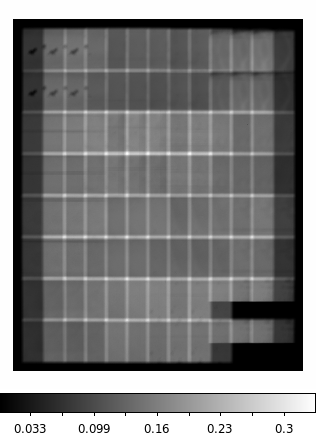
\includegraphics[width=0.5\textwidth]{Chapter2/Figs/xmm3_Ks_weights.png}
\caption[Example weight map]{Weight map for the $K_{s}$-band in the xmm3 tile. Weight values are displayed on a linear scale indicated by the bar. The two black regions in the bottom right corner are due to time-varying quantum efficiency in detector 16. Because flat fielding in that detector is extremely challenging, data from those regions has been assigned zero weight. In the top right a small region has lower weights due to dead pixels in detector 1.}
\label{fig:weight_map}
\end{figure}




In spite of the small divergent regions described above and in the caption to Figure \ref{fig:weight_map}, the overall coverage within a VIDEO tile is fairly uniform. However, even though the tiles themselves are much more uniform than the DES imaging, the VIDEO survey still contains some depth variation between tiles. This is due to the fact that the survey was not yet completed for the data release used in this thesis, so not all tiles had yet been allocated the same exposure time. To explore the variation of VIDEO depths in the \DESVIDEO catalogue, the author computed the $5\sigma$ limiting magnitudes in a \SI{1.95}{\arcsec} aperture for each tile. The procedure for calculating these values is as follows. Firstly, the $5\sigma$ limiting fluxes $F_{5\sigma}$ are derived. Because $F_{5\sigma}$ is simply defined as the flux for which the signal-to-noise ratio (S/N) equals 5, the following equation holds:


\begin{equation}
\mathrm{S/N} \equiv \frac{F_{5\sigma}}{F_{\mathrm{error}}} = 5,\label{eqn:video_signal_noise}
\end{equation}

\noindent where $F_{\mathrm{error}}$ is the VIDEO flux error in a \SI{1.95}{\arcsec} aperture. It follows that $F_{\mathrm{error}}$ can therefore be used to obtain the corresponding limiting flux $F_{5\sigma}$. Section \ref{subsubsection:error_discussion} will describe the way those uncertainties are computed for the \DESVIDEO catalogue in this thesis. The method involves an approximation whereby flux errors in a given aperture are assigned a constant value throughout each VIDEO tile. Because this approximation entails that $F_{\mathrm{error}}$ is constant, for each tile the limiting fluxes can be computed via a single instance of Equation \ref{eqn:video_signal_noise}. The limiting fluxes are then converted into magnitudes to obtain the  the final depths in each tile: 


\begin{equation}
m_{5\sigma} = m_{\mathrm{zp}} - 2.5\log{F_{5\sigma}} = m_{\mathrm{zp}} - 2.5 \log{\left( 5F_{\mathrm{error}} \right)},\label{eqn:m_n_video}
\end{equation}

\noindent where $m_{\mathrm{zp}}=-48.6$ is the AB zero-point. Table \ref{table:VIDEO_depths} shows the range in VIDEO depths derived in this way, listing the magnitude in the shallowest and deepest tiles for each filter. \par 


\begin{table}[!htb]
\centering
\textsc{VIDEO $5\sigma$ limiting magnitudes} \\
\vspace{0.1em}
\footnotesize
\begin{tabular}{lc}
\toprule\toprule
Filter &  $5\sigma$ Depth (\si{\magab}) \\
\midrule
$Z$ & 24.8 - 25.3 \\
$Y$ & 24.6 - 24.9 \\
$J$ & 23.9 - 24.6 \\
$H$ & 23.3 - 24.1 \\
$K_{s}$ & 22.9 - 23.8 \\
\bottomrule
\end{tabular}
\vspace{1em}
\caption[Minimum and maximum depths in the VIDEO data]{Minimum and maximum VIDEO $5\sigma$ depths in a \SI{1.95}{\arcsec} aperture in the \DESVIDEO catalogue. These limiting magnitudes were estimated from the catalogue photometric errors as described in the text. Depths were approximated to be constant across tiles, and the range of depths observed originates from variation between tiles. Depth variation occurs because in the data release used in this thesis the full survey depth has not been achieved in all tiles. }
\label{table:VIDEO_depths}
\end{table}

\paragraph{Weight flags} Weight flags for the VIDEO portion of the \DESVIDEO catalogue are produced by \texttt{SExtractor} during the extraction of forced photometry (see Section \ref{subsubsection:forced_phot_extraction}). As with the DESDM catalogues, non-zero weight flags identify objects that contain or touch pixels with zero weight in the co-add weight maps. For the VIDEO data, these are pixels at the very edge of the imaging and in the regions covered by detector 16 (see the bottom right of Figure \ref{fig:weight_map}). In the same way as for DES, this thesis uses the VIDEO weight flags to filter out artefacts and objects with unreliable photometry, during the computation of photometric redshift and the selection of high-redshift galaxies (see Sections \ref{subsection:photoz_computation_method} and \ref{subsubsection:weight_flag_cut} respectively).  \par


\subsection{Spectroscopic redshifts}\label{subsection:spectra}
To complement the broadband imaging and catalogues, the DES collaboration has compiled a master spectroscopic catalogue of publicly available galaxy spectra that overlap the DES footprint, published in the DES Science Portal database\footnote{\color{blue} http://cdcvs.fnal.gov/redmine/projects/des/wiki/SciencePortalProducts} \citep{2018A&C....24...52F}. This thesis uses the final \texttt{Y1A1} version (from 25 January 2016), with DESDM table name \texttt{brportal.e\_10022146\_295159}.  \par

%I GOT UP TO HERE
The master catalogue includes \num{759 535} galaxy spectra from 31 public surveys in the literature, and contains good quality flags for all objects. However, a quick investigation of the spectra revealed that some galaxies from the EBOSS survey\footnote{The source name for this survey is  \texttt{DES\_EBOSS\_ELG} in the master catalogue.} have unreliable redshifts. These objects have been assigned spectroscopic redshifts of $z_{\mathrm{spec}}>3.0$, while the DES imaging clearly indicates that they are bright ($z_{\mathrm{AB}}\lesssim20$) resolved galaxies, implying they cannot be at such high redshifts. For this reason, it was decided to remove all 335 EBOSS objects with $z_{\mathrm{spec}}>3.0$ from the master catalogue, so that \num{759 200} galaxies remain. These objects are later matched to the \DESVIDEO sources by position (within a \SI{1}{\arcsec} radius), via a process described in Section \ref{subsection:photoz_computation_method}. This matching strategy also removes any spectra with bad \texttt{FLAGS\_WEIGHT} values in any \DESVIDEO filter. At the end, these steps produced a final sample of \num{35596} galaxy spectra with \DESVIDEO photometry. The 21 spectroscopic surveys from which these spectra have been sourced are listed in Table \ref{table:spectra}, together with the fractional contribution of each survey to the total number of \DESVIDEO spectroscopic redshifts. \par 


\begin{table}[!htb]
\centering
\textsc{Sources of spectroscopic redshifts} \\
\vspace{0.1em}
\footnotesize
\begin{tabular}{lclc}
\toprule\toprule
Survey  & \% of total redshifts & Survey & \% of total redshifts \\
\midrule
3DHST & 18.9 \% & SNLS\_FORS & 1.3 \% \\
DES\_AAOMEGA & 16.5 \% & SPARCS & 0.8 \% \\
VVDS & 12.8 \% & VUDS & 0.3 \% \\
ACES & 11.9 \% & 2DF & 0.3 \% \\
GAMA & 9.6 \% & SNLS\_AAO & 0.3 \% \\
EBOSS\_DES\_ELG & 9.2 \% &  STALIN & 0.2 \% \\
NOAO\_OZDES & 8.5 \% & CDB & 0.2 \% \\
UDS & 3.5 \% & 6DF & < 0.1 \% \\
PANSTARRS & 2.4 \% & MOSFIRE & < 0.1 \% \\
ATLAS & 1.6 \% & LCRS & < 0.1 \% \\
SDSS\_OZDES & 1.5 \% & & \\

\bottomrule
\end{tabular}
\vspace{1em}
\caption[Spectra and source surveys]{Publicly available spectroscopic redshift surveys that make up the spectra in the \DESVIDEO catalogue. Spectra have been sourced from the final \texttt{Y1A1} catalogue described in the text. The names in the `Survey' column correspond to the \texttt{SOURCE} tag in this table.}
\label{table:spectra}
\end{table}

Figure \ref{fig:spectra} shows the redshift distribution of the \DESVIDEO spectra, for both the entire dataset and the ELAIS-S1, XMM-LSS, and CDF-S fields individually. With regard to the high-redshift galaxy search later in this thesis, it is important to note that the vast majority of spectra are concentrated at $z_{\mathrm{spec}}<1.0$, with only 11 at $z_{\mathrm{spec}}>4.0$ and none at $z_{\mathrm{spec}}>5.0$. The absence of available spectra at high redshifts impacts the photometric redshift strategy in Chapter \ref{chapter:photometric_redshifts}. \par 


\begin{figure}[!htb] 
\centering    
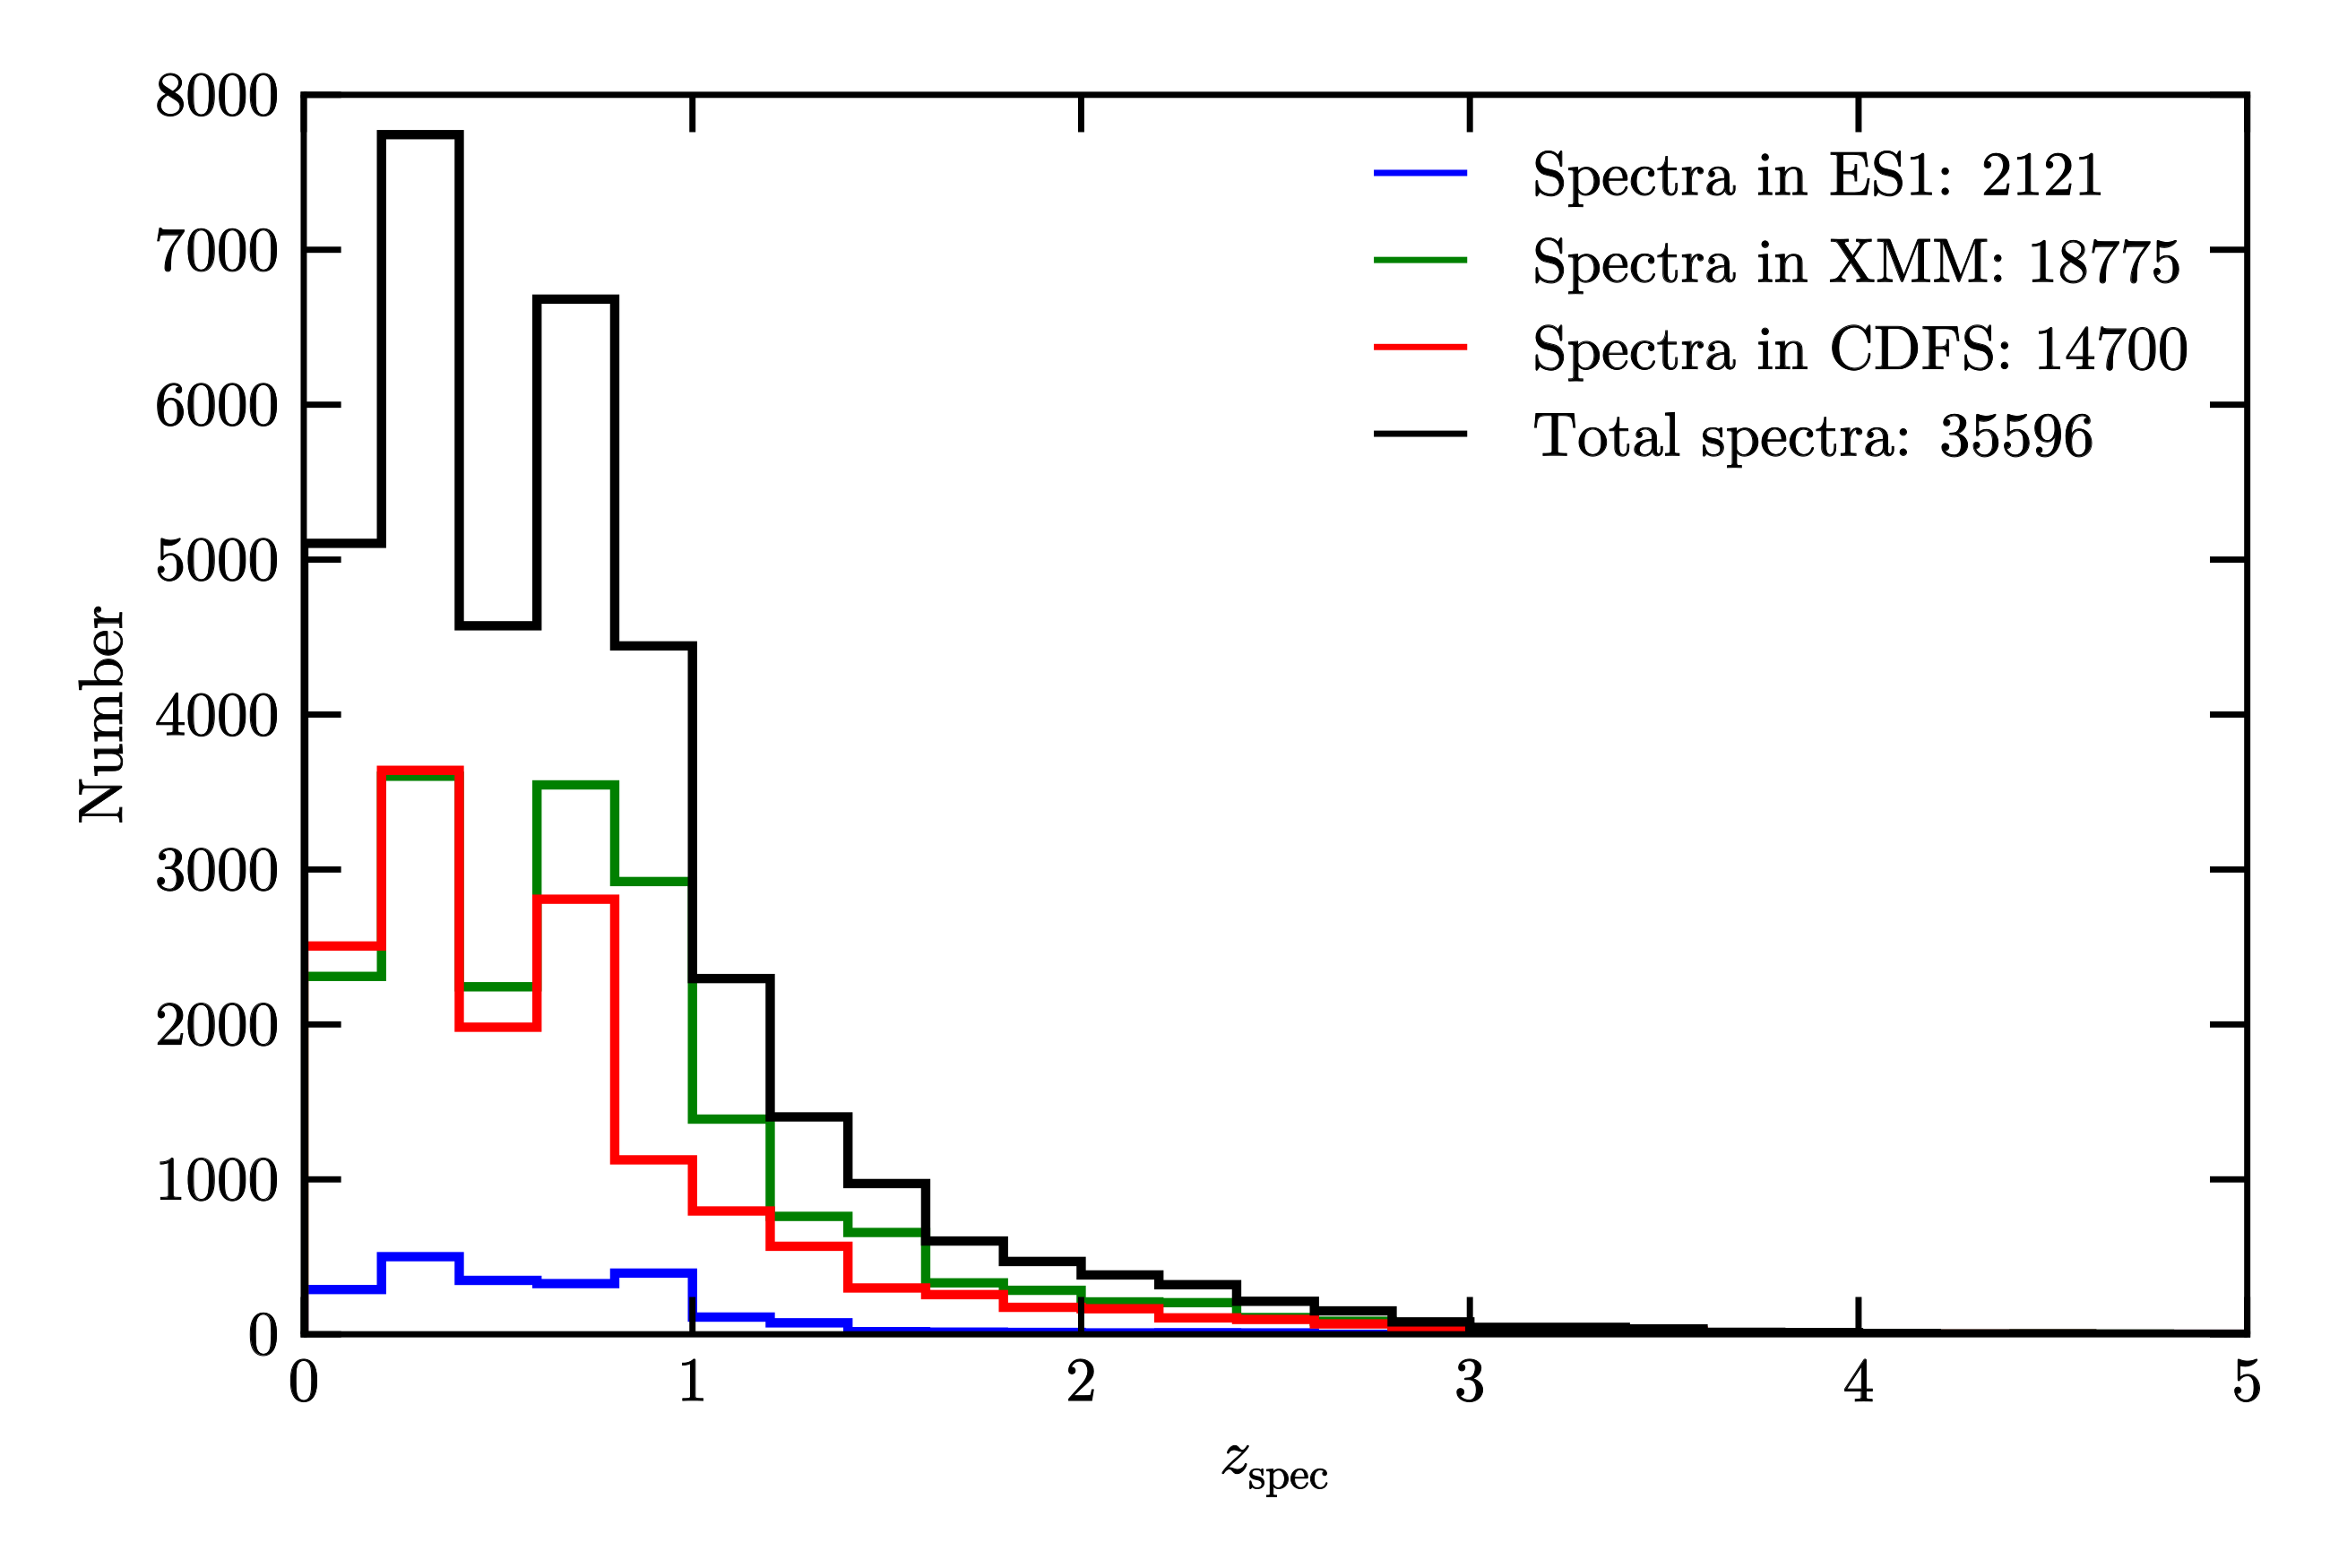
\includegraphics[width=0.95\textwidth]{spectra.png}
\caption[\texorpdfstring{$z_{\mathrm{spec}}$}{} distribution of available spectroscopic redshifts]{Spectroscopic redshift distribution of all spectra in the \DESVIDEO catalogue. The red, blue, and green histograms show the contributions from the ES1, XMM, and CDFS fields respectively, and the black histogram shows the combined distribution of all spectra. All histograms are plotted in redshift bins of $\Delta z_{\mathrm{spec}} = 0.2$.}
\label{fig:spectra}
\end{figure}






%********************************** %Fourth Section  **************************************
%\DESVIDEO CATALOGUE DOES ERRORS PER TILE. NOTE THAT THIS IS AN IMPROVEMENT OVER VIDEO CATALOGS, BECAUSE THEY DO IT PER FIELD. 

%Now the DES and VIDEO datasets have been introduced, the upcoming part of this chapter will describe how these surveys were merged into a single combined catalogue.

%\footnote{In fact, thanks to the slightly smaller PSF, the VIDEO resolution is actually somewhat better.}

\section{Forced photometry and catalogue production}\label{section:forced_photometry}
\subsection{Motivation}\label{subsection:forced_phot_motivation} Now the DES and VIDEO datasets have been introduced, the upcoming part of this chapter will turn to the next step: merging these surveys into a single combined catalogue. The most straightforward way to achieve this merger would simply be to match the existing DES and \cite{2013MNRAS.428.1281J} VIDEO catalogues by position. However, the high quality of the DES data makes it possible to do better. By using a so-called \textit{forced photometry} approach, this thesis aims to extract more information from the VIDEO imaging than is possible with VIDEO alone. The concept behind forced photometry is to use imaging from a deeper or higher resolution survey to improve the photometry and positions that can be measured from shallower or lower resolution data \citep{2015MNRAS.446.2523B, 2016AJ....151...36L}. In the case of DES and VIDEO, the two surveys have fairly similar resolutions, so the potential for improvement mainly revolves around the higher depths in the DES imaging. As demonstrated in Table \ref{table:VIDEO_depths}, the VIDEO $Z$-band data reaches depths of $24.8<Z_{\mathrm{AB}}<25.3$. While this is similar to the $z_{\mathrm{AB}}<24.9$ DES depths over the majority of the \DESVIDEO footprint, the \SI{4.3}{\sqdeg} deepest DES regions extend to $z<26.2$, which is considerably deeper. Additionally, the combined $r+i+z$ is deeper than the $z$-band alone, as it enjoys the combined exposure times from the $r$, $i$ and $z$ imaging. Therefore, it is possible to use the deeper DES imaging to obtain secure detections for objects that would be too faint to pass the detection threshold in the VIDEO imaging alone. By extracting forced photometry from VIDEO based on these secure DES detections, the VIDEO measurements can be pushed to fainter magnitudes, increasing the number of sources with measured VIDEO fluxes. The concept is illustrated in Figure \ref{fig:forced_photometry_des_cat}, which shows the increase in VIDEO measurements that can be achieved with forced photometry based on DES. Furthermore, in addition to the fact that it allows VIDEO fluxes to be obtained for fainter sources, forced photometry has a second benefit for this thesis. As mentioned in Section \ref{subsubsection:data_reduction}, the optical component of the \DESVIDEO catalogue consists of the DESDM catalogues. In order to maximise the amount of information contained within the combined catalogue, it is important to obtain VIDEO photometry for as many of these DESDM sources as possible. Forced photometry helps to achieve this objective, because it can measure VIDEO fluxes for all sources detected in DES. \par  


To extract the forced photometry and to merge it with DES data, the author has created an automated pipeline. The rest of this section will describe this pipeline and the catalogue assembly process in general. The first part will present the implementation of forced photometry, the second part will report on the validation of this method, and the third part will describe the derivation corrected photometric uncertainties for the catalogue. Then, after these parts have identified and verified the necessary steps, the fourth section will summarise the automated pipeline to produce the desired \DESVIDEO catalogue. \par



\begin{figure*}[!htpb]
\centering
\subfloat[DES detection\label{fig:forced_photometry_des_det}]{
	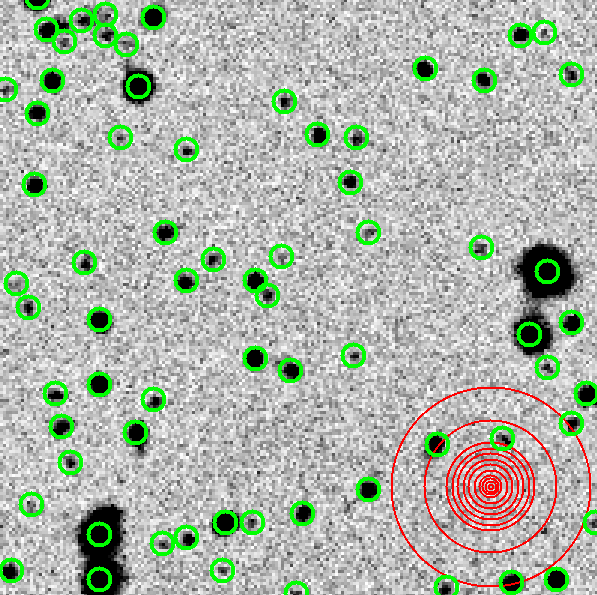
\includegraphics[clip, width=0.32\textwidth]{Chapter2/Figs/des_det_cdfs_cut.png}}
\subfloat[\DESVIDEO]{
	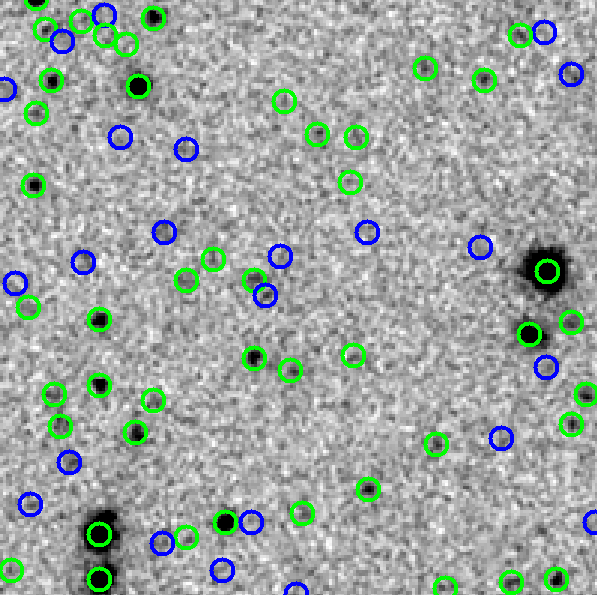
\includegraphics[clip, width=0.32\textwidth]{Chapter2/Figs/video_Z_cdfs_cut.png}}
\subfloat[VIDEO only]{
	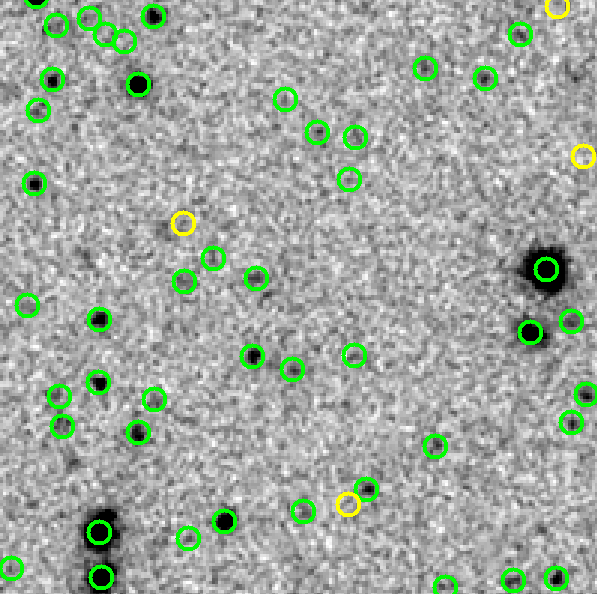
\includegraphics[clip, width=0.32\textwidth]{Chapter2/Figs/video_Z_cat_cdfs_cut.png}}
\caption[Forced photometry]{An illustration of the effectiveness of forced photometry in a section of the CDF-S where the DES data is significantly deeper than VIDEO. \textbf{(a)} DES $r+i+z$ detection image with \SI{1.95}{\arcsec} apertures centred on DES $r+i+z$ detections. All twelve aperture sizes in the \DESVIDEO catalogue (see Table \ref{table:aperture_sizes}) are superimposed to scale in red. \textbf{(b)} VIDEO $Z$-band image with DES detections from (a). The blue circles show sources which are detected in DES but not included in the VIDEO \cite{2013MNRAS.428.1281J} catalogue. \textbf{(c)} VIDEO $Z$-band image with detections from the \cite{2013MNRAS.428.1281J} VIDEO catalogue, based on the longest wavelength detection in the VIDEO $Y$-, $J$-, $H$- or $K_{s}$-band. Sources which are included in the \cite{2013MNRAS.428.1281J} catalogue but not detected in DES are shown in yellow. The abundance of blue circles compared to yellow circles illustrates that by using the deeper DES data, photometry can be obtained for VIDEO sources that are too faint to be detected in the VIDEO imaging.}
\label{fig:forced_photometry_des_cat}
\end{figure*}

%because the forced photometry is eventually measured per DES co-add tile...

\subsection{Method}\label{subsection:forced_phot_preparation}
\subsubsection{Image resampling and preparation}\label{subsubsection:image_resampling}
Before forced photometry can be extracted, the imaging must be suitably prepared. In the \DESVIDEO combination pipeline, this is achieved in the following way. Because the pipeline eventually measures forced photometry per DES co-add tile --- for every combination of intersecting DES and VIDEO tiles --- every VIDEO tile that overlaps a given DES tile is resampled to match the position, pixel scale, and size of that DES tile. This is achieved via \texttt{SWarp} v.2.38.0 \citep{2002ASPC..281..228B,2010ascl.soft10068B}, using a \texttt{LANCOS3} kernel to rescale the VIDEO data from the VIDEO pixel scale of \SI{0.2}{\arcsec.pix^{-1}} to the DES scale of \SI{0.263}{\arcsec.pix^{-1}}. Resampling is performed for every available VIDEO filter, and the \texttt{SWarp} configuration file used for this process is shown in Appendix \ref{appendix:swarp}. The result is a series of VIDEO tiles covering the same \SI{0.73 x 0.73}{\sqdeg} regions as the corresponding DES tiles. If a VIDEO tile does not fully overlap a given DES tile, \texttt{SWarp} sets the pixel values in the image and weight map to 0 in the areas where no VIDEO data is present. \par 


For the DES imaging, preparation requires consideration of the overlap pattern between the DES and VIDEO tiles. There are two special cases, which are both addressed by the pipeline. The first case applies if a DES tile is not fully contained within a given VIDEO tile, i.e. if it lies on an edge. For those tiles, the pipeline trims the DES $r+i+z$ detection image to the size of the overlapping VIDEO image. The second case concerns DES tiles where there is data from multiple VIDEO tiles. In those tiles the pipeline duplicates the detection image for each VIDEO tile and cuts  the duplicates down to the overlapping regions. This trimming is performed based on the resampled VIDEO $K_{s}$-band weight map, which was chosen because it is observed in every tile. After overlap has been accounted for, the pipeline then finishes the data preparation by assigning a value of \texttt{NaN} to all DES detection image pixels for which the corresponding VIDEO weight map pixels are zero. These zero weights occur a) for regions at the very edge of the VIDEO tile where there are no observations, b) for regions in the resampled VIDEO tiles where there is no overlapping DES data (see the previous paragraph), and c) for regions covered by the faulty detector 16 (see Section \ref{subsubsection:data_quality_video}). This approach ensures that all detected sources lie within DES regions that overlap existing and reliable VIDEO data, since the forced photometry code does not allow detected sources to contain \texttt{NaN} values. \par 


\subsubsection{Source extraction}\label{subsubsection:forced_phot_extraction}
As explained previously in Section \ref{subsection:forced_phot_motivation}, one of the advantages of forced photometry is that it can allow VIDEO fluxes to be measured for a maximum number of sources in the DESDM catalogues. To make full use of this strength, the \DESVIDEO catalogue pipeline must therefore replicate the DESDM source detection process as closely as possible, so that the measured VIDEO objects are a close match to the DESDM objects. Unfortunately, the photometry in the DESDM pipeline was obtained with a special of \texttt{SExtractor} that the author does not have access to, so it is not possible to copy that source detection method outright. In spite of this, the author has obtained a very close approximation to the DESDM results (as will be shown in Section \ref{subsection:source_extract_validation}) via a description of the DESDM configuration file, obtained from internal communication with the DES collaboration. Together with the relevant DES, VIDEO, and \texttt{SExtractor} documentation in the literature, this internal communication helped to inform the source extraction method for the \DESVIDEO pipeline. A summary of the adopted approach is presented below. \par 

Forced photometry is extracted in every available VIDEO filter, by running \texttt{SExtractor} v.2.19.5 \citep{1996A&AS..117..393B} in dual image mode for each overlapping \DESVIDEO tile combination. This process uses the DES $r+i+z$ co-adds (prepared as described in the previous section) as detection images, and the corresponding resampled VIDEO tiles as measurement images. Appendix \ref{appendix:sextractor} shows the \texttt{SExtractor} configuration file used in this process. With this setup, \texttt{SExtractor} measures photometry through a series of steps. A summary of this process, including the configuration choices made for this thesis, is presented below. More information can be found in the \texttt{SExtractor} documentation\footnote{\color{blue} http://www.astromatic.net/pubsvn/software/sextractor/trunk/doc/sextractor.pdf}. \par

Firstly, \texttt{SExtractor} creates a background map for both the DES detection and VIDEO measurement images. To do this, it estimates the background in a grid of $16 \times 16 = 256$ pixel boxes (the value of 256 used in this thesis has been imposed via the \texttt{BACK\_SIZE} parameter). Within these boxes, pixels brighter than $3\sigma$ above the median are iteratively clipped. To account for boxes where the background is overestimated due to bright stars, median filtering is applied to the grid, using a filter size of 3 boxes (as specified by the \texttt{BACK\_FILTERSIZE} parameter). The final background maps are obtained by smoothing the grid of boxes via a bicubic-spline interpolation. The resulting maps are then subtracted from the corresponding detection and measurement images. In parallel with the background maps, \texttt{SExtractor} produces a map of the RMS background noise, which is used to scale the input weight maps to the appropriate absolute level. \par 



 %(see the \texttt{SExtractor} documentation\footnote{\color{blue} http://www.astromatic.net/pubsvn/software/sextractor/trunk/doc/sextractor.pdf} for more information)


After substracting the background, \texttt{SExtractor} convolves the detection image  with a $\num{3 x 3}$ pixel convolution kernel. This improves the detectability of faint extended sources\footnote{\color{blue} http://www.astromatic.net/pubsvn/software/sextractor/trunk/doc/sextractor.pdf} by increasing the contrast with the background noise. The kernel file \texttt{sex.conv} used in this thesis is identical to the one used for the DESDM catalogues, and contains the following elements: 

\begin{equation}
\texttt{conv} =
 \begin{bmatrix}
 1 & 2 & 1 \\
 2 & 4 & 2 \\
 1 & 2 & 1 \\
 \end{bmatrix}.
\end{equation}



\texttt{SExtractor} then identifies source detections from the convolved background-subtracted $r+i+z$ detection images. For this thesis, the algorithm considers an object detected if it consists of six or more adjacent pixels (specified via $\texttt{DETECT\_MINAREA} = 6$) with a signal-to-noise ratio of  $1.6\sigma$ ($\texttt{DETECT\_THRESH} = 1.6\sigma$) above the local background\footnote{To be more precise, the required threshold for detection is adjusted for each pixel according to the weight map, such that each pixel must be above a a threshold $t_{i}=1.5\times\sqrt{\sigma_{i}^2}$, where $i$ denotes an individual pixel and $\sigma_{i}^2$ is the variance in that pixel as determined from the weight image.}. For blended detections consisting of overlapping sources, \texttt{SExtractor} attempts to separate the detections into subcomponents using a multi-thresholding algorithm \citep{1996A&AS..117..393B}. For this thesis, a subcomponent of a composite object is considered separate if its total integrated value is greater than 0.001 of the composite (\texttt{DEBLEND\_MINCONT}=0.001), and the maximum number of subcomponents is 32 (\texttt{DEBLEND\_NTHRESH}=32). \par




For every detected object, \texttt{SExtractor} extracts photometry from the back\-ground-subtracted VIDEO measurement images. The photometry consists of two main types of measurement: 


\begin{itemize}
    \item \textbf{Aperture photometry} is measured by counting the flux of pixels inside twelve fixed-size circular apertures, with a range of diameters between \SI{0.49}{\arcsec} and \SI{17.53}{\arcsec}. A list of all the diameters is provided in Table \ref{table:aperture_sizes}. To illustrate their sizes, the apertures are superimposed on part of a DES detection image in Figure \ref{fig:forced_photometry_des_det}. The diameters have been chosen to match the ones used by DESDM, so that all \DESVIDEO fluxes are measured in the same size apertures.  \texttt{SExtractor} outputs the fluxes and magnitudes as \texttt{FLUX\_APER} and \texttt{MAG\_APER} respectively. 
    %AUTO PHOTOMETRY IS EXTRACTED VIA
    \item \textbf{Auto photometry} employs a flexible elliptical aperture scaled to encompass (most of) the flux of a given source. The method implemented in \texttt{SExtractor} follows an approach pioneered by \cite{1980ApJS...43..305K} and adapted by  \cite{1996A&AS..117..393B}. It computes the shape of the desired elliptical aperture (i.e. the ratio between the semi-major and semi-minor axes) from the second order moments of the flux distribution in the detection image. The size of the ellipse is determined by a dimensionless quantity that \texttt{SExtractor} refers to as the Kron radius $R_{\mathrm{Kron}}$, which is a product of the first moment of the flux distribution and a scale factor $k$. For this thesis, the value of $k$ and the minimum permitted Kron radius $R_{\mathrm{Kron,min}}$ are set to values of 2.5 and 3.5 respectively (via the \texttt{PHOT\_AUTOPARAMS} parameter). \texttt{SExtractor} uses $R_{\mathrm{Kron}}$ to obtain the semi-major axis $a$ and semi-minor axis $b$ of the final scaled elliptical aperture in units of pixels:
    
    \begin{align}
    a &= R_{\mathrm{Kron}} \times \texttt{A\_IMAGE} \label{eqn:semi_major}, \\
    b &= R_{\mathrm{Kron}} \times \texttt{B\_IMAGE},\label{eqn:semi_minor}
    \end{align}
    
    \noindent where \texttt{A\_IMAGE} and \texttt{B\_IMAGE} are the aforementioned shape parameters computed from the second order moments, supplied in units of pixels. If the calculated value of $R_{\mathrm{Kron}}$ for a given source is less than $R_{\mathrm{Kron,min}}=3.5$, instead of a scaled aperture \texttt{SExtractor} uses an aperture of fixed area instead (still with an elliptical shape determined from the imaging). Its area corresponds to that of a circular aperture with a radius of 7.41 pixels ($\texttt{PHOT\_AUTOAPERS} = 7.41$)\footnote{This corresponds to a diameter of \SI{1.97}{\arcsec}, roughly equal to the seeing.}. \texttt{SExtractor} saves the resulting auto fluxes and magnitudes as \texttt{FLUX\_AUTO} and \texttt{MAG\_AUTO} in the output catalogues, together with \texttt{A\_IMAGE}, \texttt{B\_IMAGE}, $R_{\mathrm{Kron}}$ (listed as \texttt{KRON\_RADIUS}), and various other shape parameters. 
\end{itemize}

\begin{table}[!htpb]
\centering
\textsc{Aperture diameters} \\
\vspace{0.1em}
\footnotesize
\begin{tabular}{lcclc}
\toprule\toprule
\multicolumn{2}{c}{Aperture size}  & &  \multicolumn{2}{c}{Aperture size} \\
(arcsec) & (pix) & & (arcsec) & (pix) \\
\midrule
0.49 & 1.85 & & 4.87 & 18.52 \\
0.97 & 3.70 & & 5.84 & 22.22 \\
1.46 & 5.55 & & 6.81 & 25.93 \\
1.95 & 7.41 & & 7.79 & 29.63 \\
2.92 & 11.11 & & 11.68 & 44.44 \\
3.90 & 14.81 & & 17.53 & 66.67 \\
\bottomrule
\end{tabular}
\vspace{1em}
\caption[Aperture diameters]{Aperture diameters for the aperture photometry in the \DESVIDEO catalogue. The aperture sizes were chosen to match those of the DESDM catalogues, so that the \DESVIDEO photometry is measured in identical apertures.}
\label{table:aperture_sizes}
\end{table}

%\paragraph{} Photometry obtained via galaxy model fitting and PSF fitting is not included in the \DESVIDEO catalogue. The reason for this is that in order to measure these quantities, \texttt{SExtractor} requires a VIDEO PSF model, which is challenging to model because of the VIDEO observing strategy. As described in Section \ref{subsubsection:data_collection_video}, the VIDEO tiles are made up of paw-prints from six offsets, each of which is consists of contributions from 16 detectors. This entails that in regions of detector overlap, data may be composed of up to 16x6 PSFs. Without PSF homogenisation, this large number of PSF 



\subsection{Source extraction method validation}\label{subsection:source_extract_validation}
It is important to confirm that the configuration in the \DESVIDEO pipeline indeed replicates the DESDM configuration as closely as possible. To verify this, the author used the \DESVIDEO setup for a single \texttt{SExtractor} run in the DES0227-0458 tile, specifying the combined $r+i+z$ image as the detection image and the DES $z$-band image as the measurement image. The current section compares the result to the DESDM catalogue in the same tile.  \par

Within the single tile that was studied, the DESDM catalogue contains \num{126 624} detected sources, whereas the \DESVIDEO method in this thesis --- let us refer to this as the `Schooneveld configuration' --- finds \num{126 980} sources. When merging these catalogues by position\footnote{Based on the \texttt{ALPHAPEAK\_J2000} and \texttt{DELTAPEAK\_J2000} output parameters.} within a \SI{1}{\arcsec} radius (permitting no duplicate matches), the total number of matches is \num{123 993}. The numbers imply that the DESDM catalogues contain 2631 objects ($\approx 2\%$) not detected by the Schooneveld configuration. Conversely, the Schooneveld setup produces 2987 sources ($\approx 2\%$) that are not present in the DESDM catalogues. Figure \ref{fig:z_flux_histogram} illustrates the difference in detections between the two methods as a function of magnitude. When the author inspected the images for the divergent detections, it became clear that these objects are clustered around bright stars. They are also mostly undetected or extremely faint in the $z$-band. This suggests that the difference is caused by small differences in the way the two source extraction methods handle the detection threshold in edge cases, which may have to do with the specifics of the background estimation. Possible explanations are the fact that the DESDM configuration used a different version of \texttt{SExtractor}, or a perhaps slightly different weights image. Nonetheless, compared to the $\sim127 000$ sources in the test tile, the number of $\sim3000$  divergent detections is very small, and it is overall reassuring that the two methods retrieve very similar sets of objects. \par


%INVISIBLE - was this a visual inspection thing in the images or just a low flux in the catalogues kinda thing?






The DESDM and Schooneveld configurations were also compared in terms of the position of the brightest pixel for each object (given by the \texttt{ALPHAPEAK\_J2000} and \texttt{DELTAPEAK\_J2000} parameters). The agreement was found to be excellent: 98.5\% of all detections have identical positions and 99.7\% differ by at most 1 pixel. This demonstrates that the forced photometry is working as desired, since it confirms that the detections in the Schooneveld configuration correspond to the same sources in the DESDM catalogues. Together, this result and the result from the previous paragraph show that the Schooneveld and DESDM configurations retrieve largely the same sources, almost entirely in exactly the same positions. Therefore, it is concluded that the Schooneveld configuration can indeed achieve the aim of obtaining VIDEO photometry for a maximal number of DES sources. \par  


Additionally, Figure \ref{fig:z_flux_compare} illustrates that the Schooneveld configuration also retrieves similar photometry to the DESDM configuration. It is suspected that any discrepancies are  largely due to the fact that the DESDM pipeline possibly uses a slightly different background estimation procedure. Because \texttt{SExtractor} obtains its photometry from the background-subtracted images, magnitudes are sensitive to the specifics of the subtraction process. This suspicion is corroborated by the observation that sources with a magnitude difference of $z_{\mathrm{AB,Schooneveld}}-z_{\mathrm{AB,DESDM}}>0.01$ preferentially reside in regions where the \texttt{SExtractor} \texttt{BACKGROUND} parameter diverges between the two catalogues. \par 

\begin{figure}[h] 
\centering    
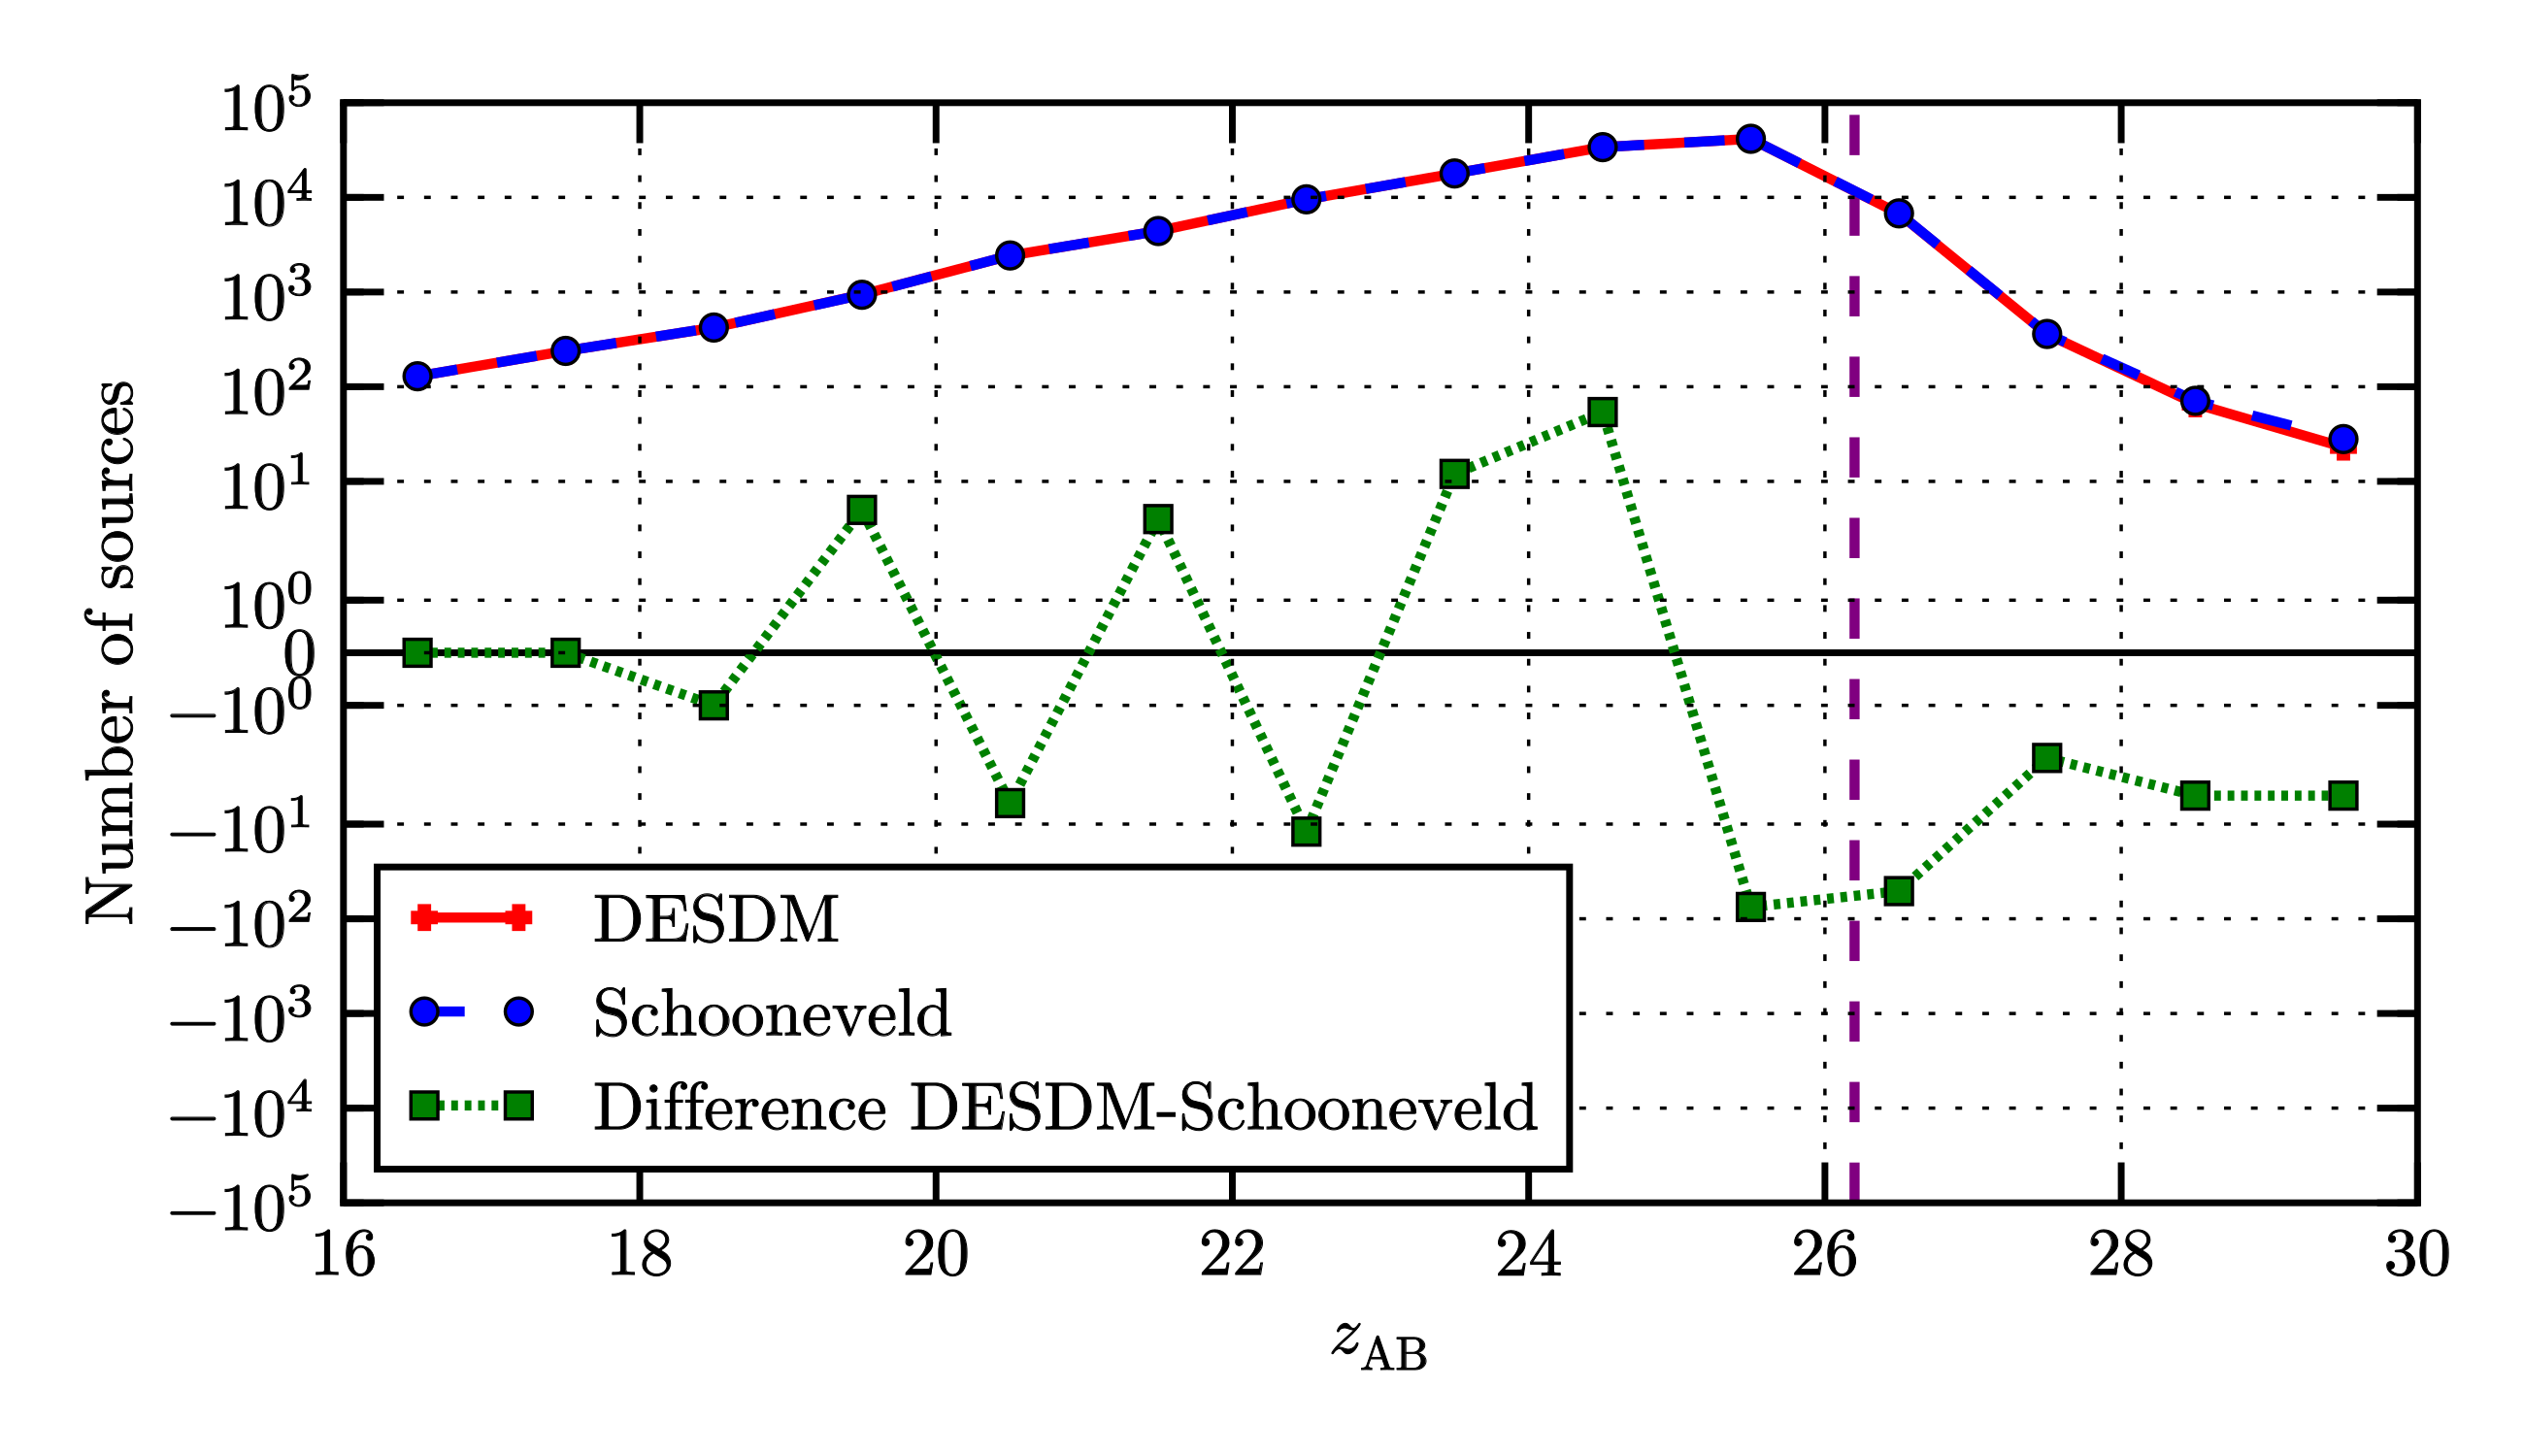
\includegraphics[width=0.95\textwidth]{z_flux_histogram.png}
\caption[Verification of the photometry method: number of source detections]{$z$-band magnitude in a \SI{1.95}{\arcsec} diameter aperture versus number of detections in bins of \SI{1}{\mag}, for detections in the DES0227-0458 tile only. Blue pluses show data from the DESDM catalogues. Green squares show the Schooneveld configuration results, from a single \texttt{SExtractor} run with the \DESVIDEO configuration used in this thesis, as described in the text. The difference between these data points is shown in red. The vertical purple dotted line shows the mean $5\sigma$ depth in the DES0227-0458 tile.}
\label{fig:z_flux_histogram}
\end{figure}


\begin{figure}[h] 
\centering    
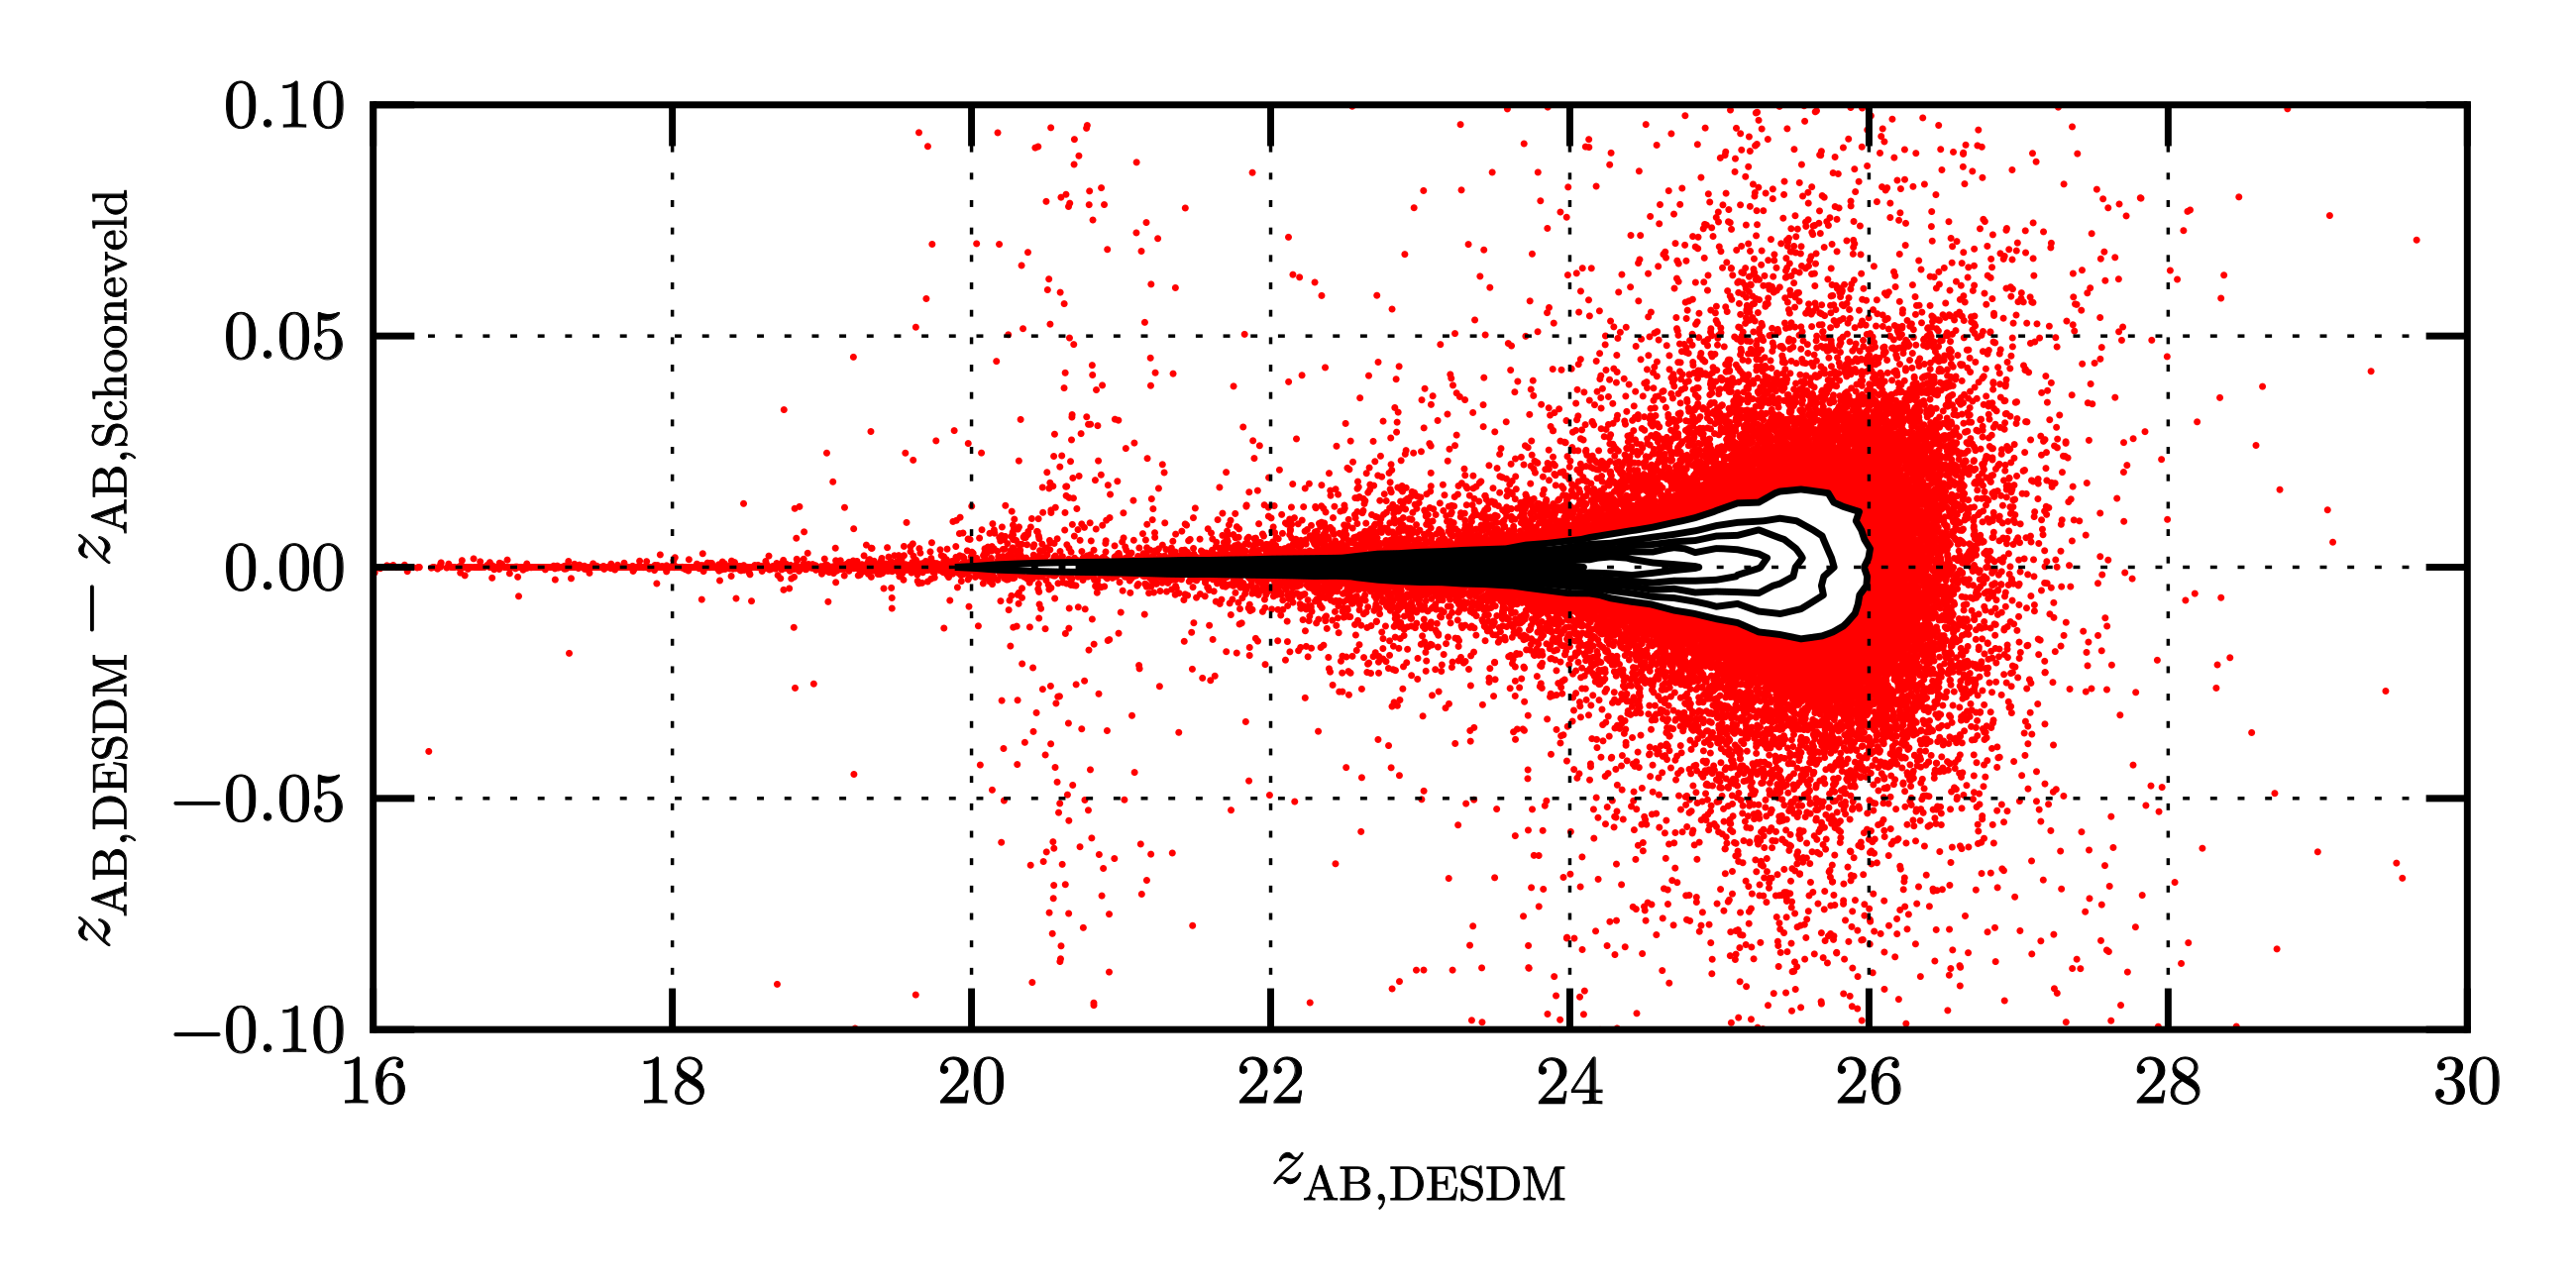
\includegraphics[width=0.95\textwidth]{z_flux_compare.png}
\caption[Verification of the photometry method: photometry]{Difference in $z$-band magnitude in a \SI{1.95}{\arcsec} diameter aperture between the DESDM configuration and the Schooneveld configuration, plotted as a function of DESDM magnitude. Both configurations contain data from the DES0227-0458 tile only. The Schooneveld configuration consists of a single \texttt{SExtractor} run with the \DESVIDEO configuration used in this thesis, as described in the text. Each plotted point corresponds to an object common to both outputs.}
\label{fig:z_flux_compare}
\end{figure}


All in all, the good degree of agreement in all three of the above tests implies that the source extraction method in this thesis is adequate for the purpose of obtaining forced photometry for the \DESVIDEO catalogue. \par 



\subsection{Correction of the VIDEO photometric uncertainties}\label{subsection:errors}
Before the VIDEO forced photometry can be incorporated into the \DESVIDEO catalogue, its uncertainties must be adjusted to the correct values. The photometric noise properties estimated by \texttt{SExtractor} assume that images are made up of uncorrelated pixels, so that the noise follows a Poisson distribution. As a result, the uncertainties listed in the \texttt{SExtractor} output catalogues are simply based on the pixel-to-pixel rms. However, this assumption of uncorrelated noise is not valid for the VIDEO images, as they have been resampled several times. The VIDEO survey data reduction process (see Section \ref{subsubsection:video_data_reduction}) initially rescaled the images from the VIRCAM pixel scale of \SI{0.339}{\arcsec.pix^{-1}} to the VIDEO co-add scale of \SI{0.2}{\arcsec.pix^{-1}}, and the resampling for this thesis (described in Section \ref{subsubsection:image_resampling}) has further rescaled the imaging to the \SI{0.263}{\arcsec.pix^{-1}} DES pixel scale. In both instances, this process has introduced correlations between pixels, which means that the  \texttt{SExtractor} errors are expected to give an inaccurate representation of the true VIDEO uncertainties (see e.g.  \citealt{2003AJ....125.1107L} and \citealt{2006ApJS..162....1G} for a demonstration that correlated fluxes lead to incorrect \texttt{SExtractor} errors). \par

 

To obtain a more accurate measure of the VIDEO errors, the author has computed the correct uncertainties via a technique developed by \cite{2003AJ....125.1107L} and \cite{2006ApJS..162....1G}, which is commonly applied in the literature (e.g. \citealt{2007AJ....134.1103Q,2011ApJ...735...86W,2013ApJS..206....8M,2013MNRAS.428.1281J}). Conceptually, this approach involves measuring the flux inside a large number of  fixed-size apertures placed randomly in empty regions of the image. The distribution of fluxes within these apertures can be approximated by a Gaussian curve. The true photometric error, which corresponds to the  background noise, can then be computed from the standard deviation of this Gaussian. \par 

Before the discussion will move on to applying this method to the data, it is important to note that correlated noise is not an issue for the DES uncertainties. Because the DES co-add pixel scale of  \SI{0.263}{\arcsec.pix^{-1}} is identical to that of the DECam CCDs, the DESDM data reduction process described in Section \ref{subsubsection:data_reduction} did not need to apply any rescaling to resample the DECam exposures into the DES co-adds. This means that the co-addition introduced only minimal flux correlations, exclusively from stacking with \texttt{SWarp}. As a result, the original \texttt{SExtractor} errors in the DESDM catalogues indeed closely capture the true photometric uncertainties, and no corrections are required. \par



\subsubsection{Aperture flux errors}\label{subsubsection:aperture_flux_errors}
The above method for correcting the VIDEO uncertainties has been implemented via a custom code developed by the author. In this algorithm, errors are calculated for each VIDEO tile and filter individually, following a process that will now be described below. Firstly, the error-calibration pipeline creates a segmentation image for each VIDEO co-add tile\footnote{For clarity, these are the original VIDEO data products presented in Section \ref{subsubsection:video_data_reduction}, before the resampling and cutting up by the \DESVIDEO pipeline described in Section \ref{subsubsection:forced_phot_extraction}.} via \texttt{SExtractor}, using essentially\footnote{The only thing that needed to be changed in the input files are the values specified for the aperture diameter, since these must be supplied in pixels. Because the VIDEO tiles have a pixel scale of \SI{0.2}{\arcsec.pix^{-1}}, the aperture sizes in these  \texttt{SExtractor} runs are scaled by a factor of $0.2/0.263=0.760$ compared to the values listed in Table \ref{table:aperture_sizes} and Appendix \ref{appendix:sextractor}. The true size of the apertures (i.e. the size in arcsec) remains the same.} the same configuration as described in Section \ref{subsubsection:forced_phot_extraction} and Appendix \ref{appendix:sextractor}.  In such segmentation maps, \texttt{SExtractor} assigns an integer value to pixels designated as part of a detected object, and a value of zero to all other pixels. An example region of such a segmentation map is shown in Figure \ref{fig:segmentation}. To identify empty regions, the pipeline firstly randomly chooses \num{500000} positions on the segmentation map. For a given aperture size the code then selects a random subset of \num{10000} positions with empty apertures (i.e. not encircling any non-zero pixels that overlap a detected object), which it uses to extract the required background fluxes from the VIDEO co-add tiles. For each tile and filter, the random selection of \num{10000} empty apertures from the \num{500000} random positions and the subsequent photometry procedure is executed seven times --- once for each of the first seven aperture sizes in Table \ref{table:aperture_sizes} (i.e. with diameters between \SI{0.49}{\arcsec} and \SI{4.87}{\arcsec}). The larger apertures are omitted, because these are more likely to encircle some low surface brightness sources just below the detection limit and are thus less reliably truly empty. Fluxes from random apertures on the very edge of a given tile (where the pixel flux values are zero) are then removed by rejecting any fluxes that equal exactly zero. The result is a series of just under\footnote{The numbers ended up as slightly less than \num{10000} because of the rejected fluxes from apertures that happened to lie on the very edge of a tile.} \num{10000} fluxes in random empty apertures for every VIDEO tile, VIDEO filter, and aperture size. \par

\begin{figure}[!tpb] 
\centering    
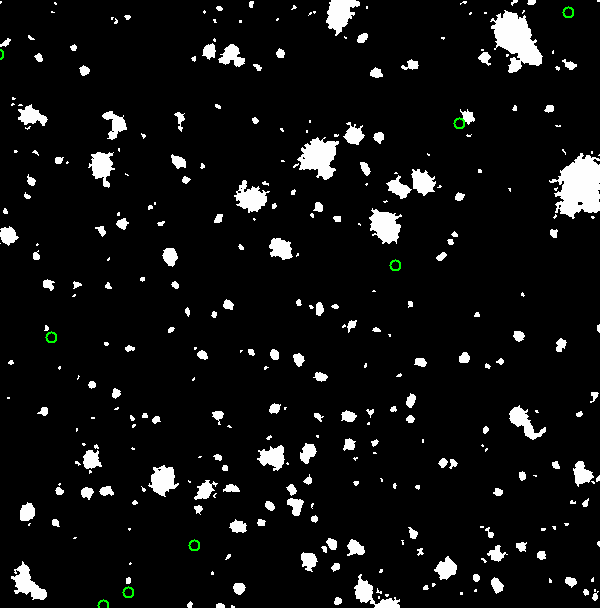
\includegraphics[width=0.45\textwidth]{aperture_errors.png}
\caption[Segmentation image]{Segmentation image for the VIDEO $K_{s}$-band in the xmm3 tile, with \SI{1.95}{\arcsec} apertures randomly placed in empty regions. The white areas consist of pixels that \texttt{SExtractor} has assigned to a detection. For the purpose of error estimations, apertures are designated as empty if they do not encircle any of these pixels.}
\label{fig:segmentation}
\end{figure}


\begin{figure*}[!tpb]
\centering
\subfloat[Flux distribution\label{fig:flux_fitting_distribution}]{
	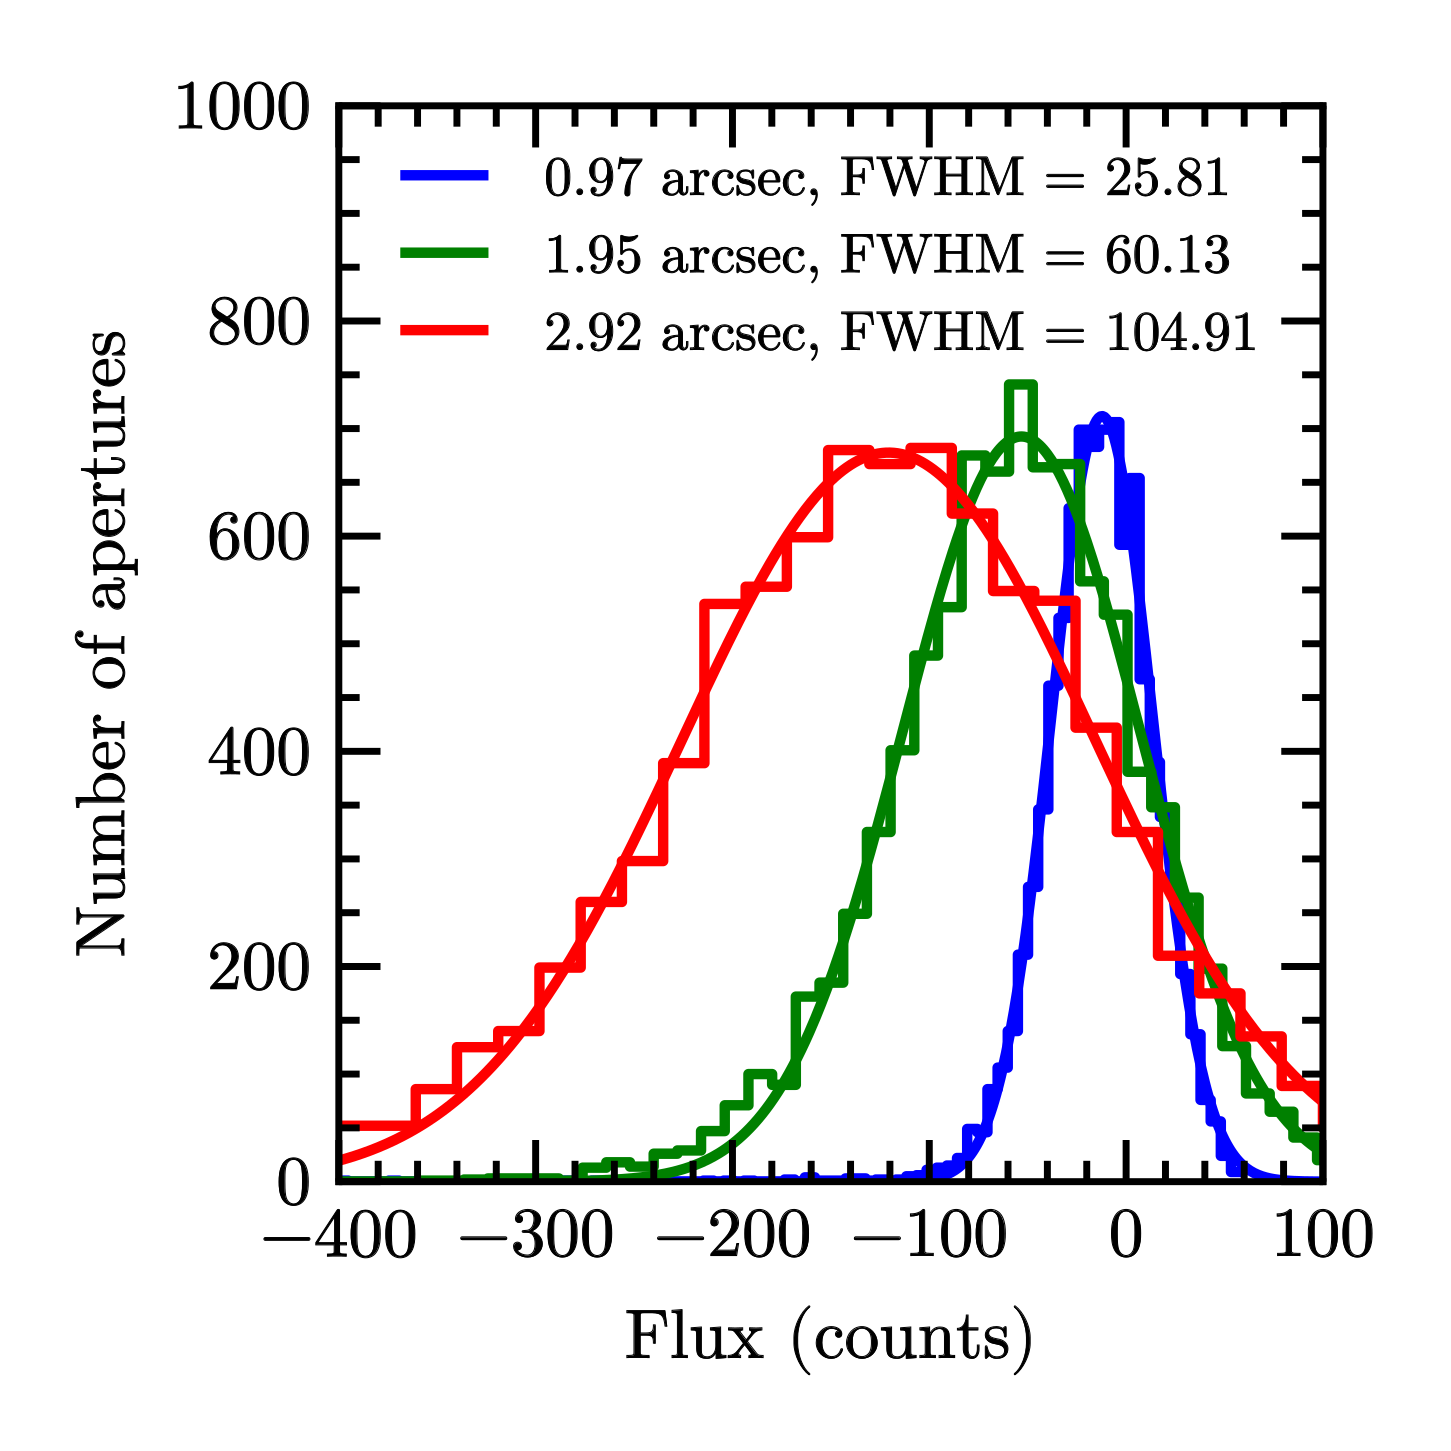
\includegraphics[clip, width=0.50\textwidth]{Chapter2/Figs/error_histogram.png}}
\subfloat[Radius dependence\label{fig:flux_fitting_radius}]{
	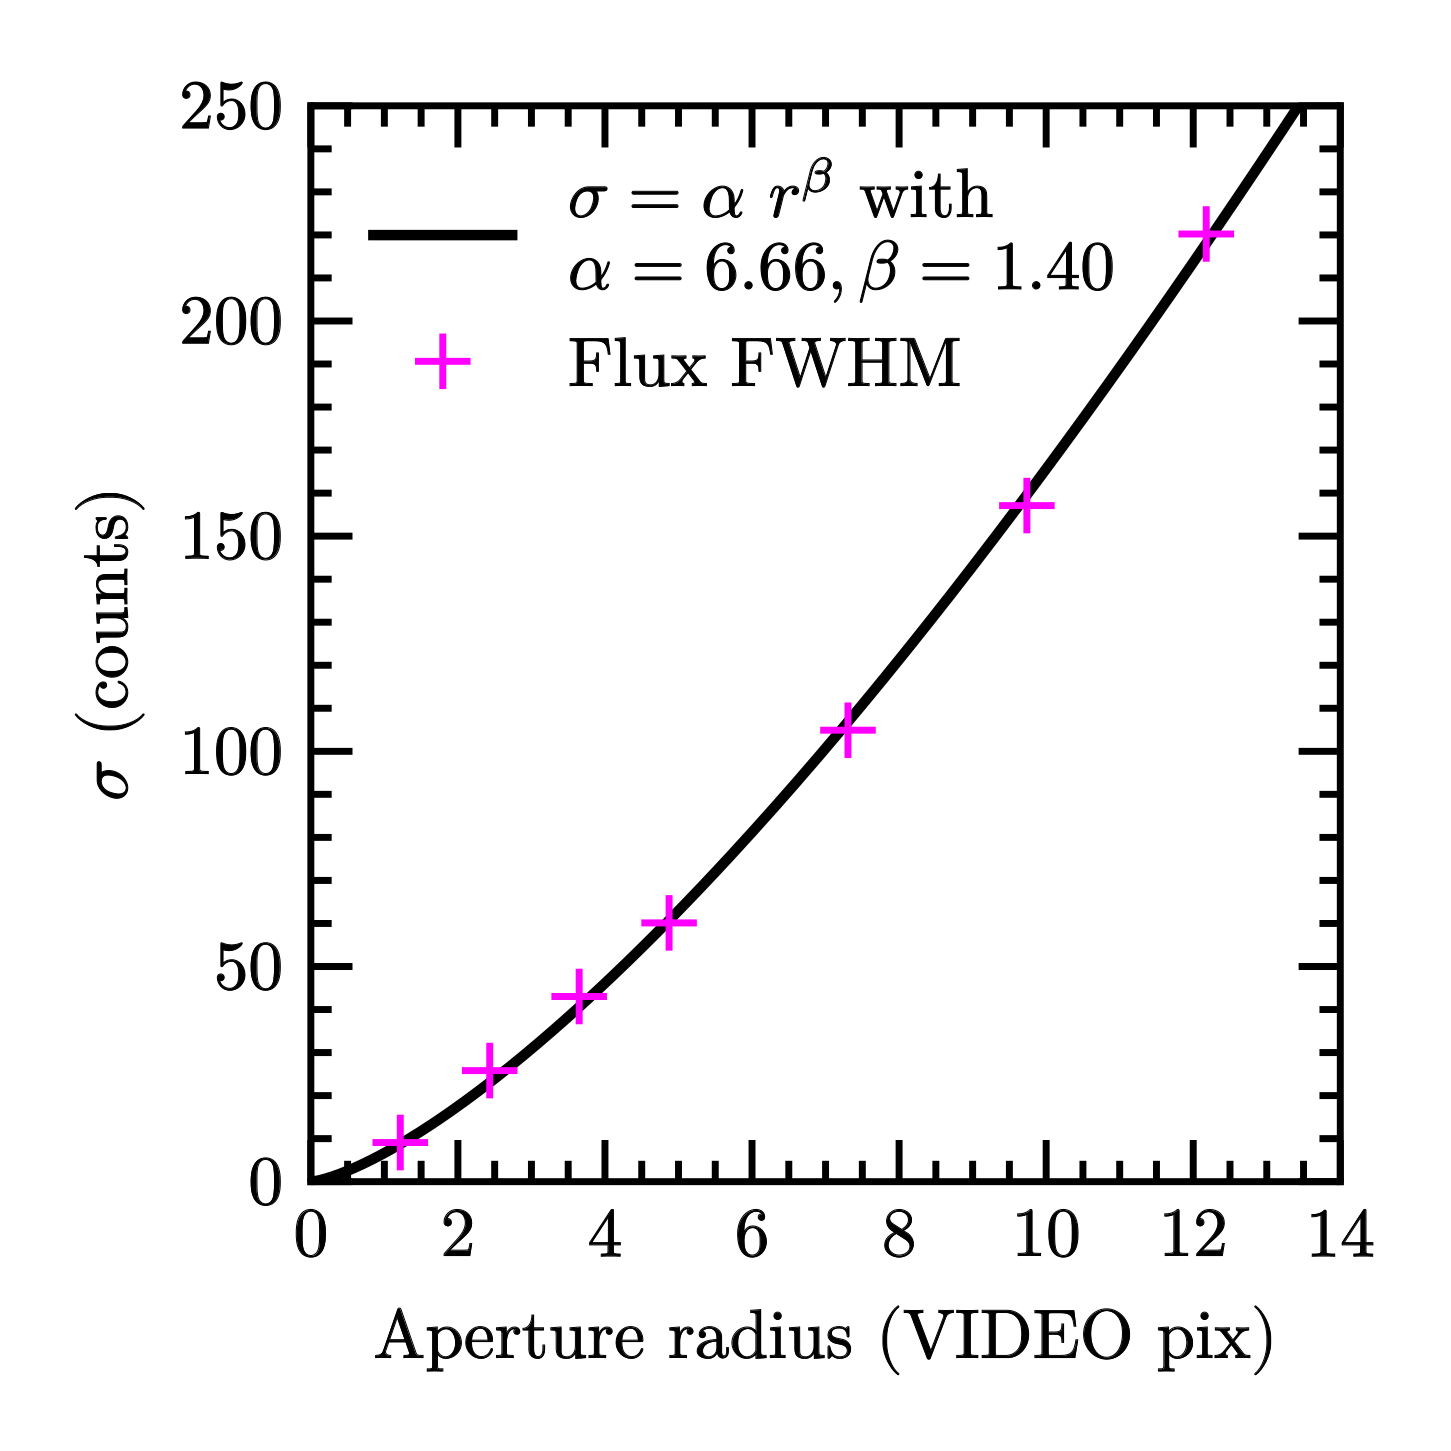
\includegraphics[clip, width=0.50\textwidth]{Chapter2/Figs/error_plot.png}}
\caption[Error estimation procedure]{An illustration of the two-part fitting algorithm to estimate VIDEO photometric errors, showing results for the $K_{s}$-band in the xmm3 tile. \textbf{(a)} Histograms of flux distributions for three of the seven measured apertures (i.e. 0.97, 1.95, and \SI{2.92}{\arcsec}; in blue, green, and red respectively), binned in intervals adjusted proportionally to the standard deviation. Each distribution has been fitted to a Gaussian, which is overplotted. For each aperture size, the measured background error $\sigma$ is equal to the Gaussian FWHM listed in the legend. \textbf{(b)} The background error $\sigma$  for all seven \SIrange{0.49}{4.87}{\arcsec} apertures as a function of aperture radius. The values of $\sigma$ (shown in pink pluses) have been computed via the Gaussian fitting prodecure illustrated in (a). Radii are given in the pixel scale of the VIDEO tiles (i.e. \SI{0.2}{\arcsec.pix^{-1}}), and the apertures from (a) correspond to the second, fourth, and fifth data points from the left.  The values of $\sigma$ have been fitted to a power law $\sigma=\alpha \ r^{\beta}$ to obtain values for $\alpha$ and $\beta$. The power law for the best-fit values of $\alpha$ and $\beta$ is shown in black. This power law is then used to calculate the final errors for all twelve \DESVIDEO aperture sizes.}
\label{fig:flux_fitting}
\end{figure*}


For each tile, filter, and aperture size, the pipeline fits a Gaussian curve to the distribution of fluxes. Figure \ref{fig:flux_fitting_distribution} illustrates this process, showing the results for the 0.97, 1.95, and \SI{2.92}{\arcsec} apertures in the xmm3 $K_{s}$-band. The standard deviation $\sigma$ of the fitted Gaussians corresponds to the desired quantity, i.e. the background error in a given aperture. It is reassuring that upon visual inspection of the pipeline fits, all the measured flux distributions were found to be fitted well by a Gaussian, as expected if the method in the \DESVIDEO pipeline indeed measures the background noise in empty regions \citep{2003AJ....125.1107L,2006ApJS..162....1G}. \par  


Up to this point, the error-estimation algorithm can successfully compute the background error for each tile and filter in the seven smallest aperture sizes. To smooth out the effects of random aperture selection for these seven sizes, as well as to obtain uncertainties for the five largest aperture sizes, the background error $\sigma$ is expressed as a function of aperture radius, from which  maximally reliable errors for all twelve aperture sizes can be interpolated and extrapolated.  Following \cite{2006ApJS..162....1G} and \cite{2011ApJ...735...86W}, this dependence of $\sigma$ on the aperture radius $r$ is parameterised by a power law: 

\begin{equation}
\sigma = \alpha \ r^{\beta}, \label{eqn:sigma}
\end{equation}

\noindent where $\beta=1$ in the case of no correlations between pixels, and  $\beta=2$ for perfect correlations. The pipeline fits this power law to the values of $\sigma$ in all seven measured apertures to obtain $\alpha$ and $\beta$. As an example, the resulting curve for the xmm3 $K_{s}$-band is shown in Figure \ref{fig:flux_fitting_radius}. Here, as well as in all other fields and filters, the output value of $\beta$ was crucially found to lie between 1 and 2, confirming the presence of correlations between pixels. \par

As a final step, the pipeline then computes the desired \DESVIDEO catalogue flux errors (\texttt{FLUXERR\_APER}) for all twelve apertures in Table \ref{table:aperture_sizes}, by inserting the best-fit parameters $\alpha$ and $\beta$ into Equation \ref{eqn:sigma}. At the same time these flux errors are also converted to magnitude errors (\texttt{MAGERR\_APER}). The resulting measurements of \texttt{FLUXERR\_APER} and \texttt{MAGERR\_APER} in every tile and filter are later used by the \DESVIDEO catalogue creation pipeline to replace the original errors computed by \texttt{SExtractor}.  \par

\paragraph{Assumptions} It is important to point out that the above process for computing the corrected VIDEO errors is based on a number of assumptions. Firstly, the error measurements assume that the uncertainties are constant within a given VIDEO tile. In practice, this is not completely true, because some parts of the tiles contain a higher or lower number of exposures than average (as described in Section \ref{subsubsection:data_quality_video}). This variation causes slight differences in the true errors, as a higher density of exposures leads to lower true background errors (and vice versa). Nevertheless, since the VIDEO coverage is reasonably uniform within each tile (as demonstrated in Figure \ref{fig:weight_map}), the assumption of constant errors is reasonably accurate. It is noted that \cite{2013MNRAS.428.1281J} have also made the same assumption. \par 

Secondly, it is assumed that the flux uncertainties can be directly equated with the background error. In reality, the true uncertainties also contain a contribution from the Poisson counting of electrons in the detectors \citep{2007AJ....134.1103Q}. However, this effect is only significant for the very brightest sources. In the \cite{2013MNRAS.428.1281J} catalogues, which do include Poisson counting, its contribution to the error only reaches >1\% at $Z_{\mathrm{AB}}<20.8$ in the $Z$-band and at $K_{s}<17.4$ in the $K_{s}$-band. The \DESVIDEO catalogue is primarily aimed at computing photometric redshifts for galaxies and finding high-redshift galaxies. Since the vast majority of these objects are significantly fainter than the threshold at which Poisson counting becomes important, the omission of the Poisson contribution is justified for the purposes of this thesis. \par 

%This threshold is much brighter than the vast majority of objects that are relevant to the objectives of the \DESVIDEO catalogue, which is aimed at computing photometric redshifts and finding high-redshift galaxies. Therefore, omitting the Poisson contribution is justified for the purposes of this thesis. 

%



\subsubsection{Auto flux errors}
In contrast to aperture photometry, which is measured in circular apertures of a fixed size, \texttt{SExtractor} measures auto photometry in elliptical apertures which are scaled to the size of each individual detection (as explained previously in Section \ref{subsubsection:forced_phot_extraction}).  By using Equation \ref{eqn:sigma}, the \DESVIDEO pipeline can also estimate accurate errors for those varying apertures. In order to do so, the error estimation code defines an `effective radius' $R_{\mathrm{eff}}$, which is the radius that corresponds to a circular aperture of the same area $A_{\mathrm{circ}}$ as the ellipse: 

\begin{equation}
    \pi R_{\mathrm{eff}} = A_{\mathrm{circ}} \equiv A_{\mathrm{ell}} = \pi a b. \label{eqn:A}
\end{equation}

\noindent Here, $A_{\mathrm{ell}}$ is the area of an elliptical aperture with semi-major and semi-minor axes $a$ and $b$. The expressions that \texttt{SExtractor} uses to calculate $a$ and $b$ have been introduced previously in Equations \ref{eqn:semi_major} and \ref{eqn:semi_minor}. Together with Equation \ref{eqn:A}, these yield:

\begin{equation}
R_{\mathrm{eff}} = \sqrt{R_{\mathrm{Kron}} \times \texttt{A\_IMAGE} \times R_{\mathrm{Kron}} \times \texttt{B\_IMAGE}}. \label{eqn:r_eff}
\end{equation}

\noindent If the Kron radius computed by \texttt{SExtractor} falls below the specified minimum value introduced in Section \ref{subsubsection:forced_phot_extraction}, the effective radius $R_{\mathrm{eff}}$ instead corresponds to that of a \SI{1.97}{\arcsec} diameter circular aperture. For each object, the error calibration pipeline computes the auto uncertainties by inserting the value of $R_{\mathrm{eff}}$ into Equation \ref{eqn:sigma}, using the best-fit parameters $\alpha$ and $\beta$ computed from the flux FWHM in circular apertures as described in Section \ref{subsubsection:aperture_flux_errors}. The resulting auto errors and corresponding magnitude errors later replace the \texttt{FLUXERR\_AUTO} and \texttt{MAGERR\_AUTO} uncertainties computed by \texttt{SExtractor}. Similarly to the aperture flux procedure, the auto flux calibration assumes that the background is constant within a tile, and that the contribution from Poisson counting is insignificant. \par 



\subsubsection{Verification of the corrected errors}\label{subsubsection:error_discussion}


\begin{table}[!p]
\centering
\textsc{\DESVIDEO errors compared to \cite{2013MNRAS.428.1281J}} \\
\vspace{0.1em}
\footnotesize
\begin{tabular}{lcccccccc}
\toprule\toprule
& \multicolumn{2}{c}{Error}  & &  \multicolumn{2}{c}{Error} & &  \multicolumn{2}{c}{Error} \\
& \multicolumn{2}{c}{(\SI{2}{\arcsec} aperture)}  & &  \multicolumn{2}{c}{(\SI{2}{\arcsec} aperture)} & &  \multicolumn{2}{c}{(\SI{2}{\arcsec} aperture)} \\
& \multicolumn{2}{c}{(counts)}  & &  \multicolumn{2}{c}{(counts)} & &  \multicolumn{2}{c}{(counts)} \\
\vspace{-0.7em}\\
\toprule
& \multicolumn{2}{c}{$Z$-band}  & &  \multicolumn{2}{c}{$Y$-band}  & &  \multicolumn{2}{c}{$J$-band} \\
Tile & Schooneveld & Jarvis &  & Schooneveld  & Jarvis & & Schooneveld  & Jarvis \\
\midrule\midrule
cdfs1 & 24.4 & 24.8 & & 31.2 & 31.3 & & 31.6 & 32.2 \\
cdfs2 & - & - & & - & - & &  44.7 & 46.5 \\
cdfs3 & - & - & & - & - & &  48.7 & 51.1 \\
es1-north & 15.3 & 14.5 & & 22.7 & 21.2 & & 56.4 & 60.6 \\
es1-south & 17.3 & 16.9 & & 27.7 & 27.1 & &  57.0 & 62.2 \\
xmm1 & 14.0 & 13.0 & & 22.6 & 21.6 & & - & - \\
xmm2 & - & - & & 22.9 & 22.2 & & 30.6 & 31.3 \\
xmm3 & 15.0 & 13.6 & & 22.6 & 21.6 & & 30.3 & 30.6 \\
\midrule
& \multicolumn{2}{c}{$H$-band}  & &  \multicolumn{2}{c}{$K_{s}$-band} \\
Tile & Schooneveld & Jarvis & & Schooneveld  & Jarvis & & &  \\
\midrule\midrule
cdfs1 & 49.7 & 51.1 & & 66.0 & 68.8 & & & \\
cdfs2 & 101.9 & 109.9 & & 73.9 & 76.3 & & & \\
cdfs3 & - & - & & 140.2 & 151.6 & & & \\
es1-north & 53.6 & 54.0 & & 63.6 & 66.0 & & & \\
es1-south & 47.2 & 47.7 & & 64.2 & 67.8 & & & \\
xmm1 & 64.2 & 67.4 & & 70.1 & 72.1 & & & \\
xmm2 & 45.8 & 47.0 & & 67.4 & 70.4 & & & \\
xmm3 & 46.8 & 48.0 & & 63.4 & 66.7 & & & \\
\bottomrule
\end{tabular}
\vspace{1em}
\caption[Comparison of photometric uncertainties]{A comparison between the VIDEO errors computed via the procedure in this thesis (labelled `Schooneveld') and the errors from the \cite{2013MNRAS.428.1281J} catalogues. The \cite{2013MNRAS.428.1281J} errors in this table include the random background error only (i.e. they do not contain the contribution from Poisson counting of electrons in the VIRCAM detectors). Dashes indicate filters which were not observed in a given tile. Since \cite{2013MNRAS.428.1281J} photometry used a \SI{2}{\arcsec} diameter aperture, the Schooneveld errors have been scaled from the DES radius of \SI{0.97}{\arcsec} to the VIDEO radius of \SI{1}{\arcsec} via Equation \ref{eqn:sigma} --- i.e. $\sigma_{\mathrm{2arcsec}} = \sigma_{\mathrm{1.95arcsec}} (1/0.97)^{\beta}$. The values of $\beta$ for each filter and tile have been derived from the best-fit parameters of Equation \ref{eqn:sigma}, which have been obtained as described in Section \ref{subsubsection:aperture_flux_errors}. The agreement between all pairs of errors is generally good, with all values agreeing within 10\% and a majority within 5\%. }
\label{table:error_agreement}
\end{table}

 

To verify that the error estimation algorithm in this thesis functions as intended, the author has compared its output to the errors in the \cite{2013MNRAS.428.1281J} catalogues (which were similarly empirically determined from the standard deviation of flux in randomly placed apertures). Table \ref{table:error_agreement} presents the results of this comparison. Reassuringly, the agreement is generally good. In all tiles and filters, the two error values agree within $<10 \%$, with most differing by less than 5\%. \par

The corrected errors were also compared to the original (uncorrected) \texttt{SExtractor} errors. The analysis revealed a considerable difference, with \texttt{SExtractor} underestimating the uncertainties by up to a factor of 2 in some filters. This observation quantitatively underlines the extent to which flux correlations introduced by image resampling can cause problematic inaccuracies in error estimations that are simply based on pixel-to-pixel rms. It therefore confirms that if such resampling has occurred, other measurement techniques, such as the empty apertures method pioneered by \cite{2003AJ....125.1107L} and \cite{2006ApJS..162....1G} and implemented in this thesis, must be used to identify the errors accurately. \par 



\subsection{Combined \DESVIDEO catalogue production pipeline}\label{subsection:catalog_production}
Now all the necessary sub-procedures for compiling the \DESVIDEO catalogue have been introduced, this section presents the algorithm that combines them into a single data processing pipeline. It consists of the following steps: 

\begin{enumerate}
    \item Firstly, the pipeline prepares the images via the procedure presented in \ref{subsubsection:image_resampling}, resampling the VIDEO tiles to the size and pixel scale of the DES tiles and trimming the DES tiles to the overlap of each VIDEO tile. 
   
    %Firstly, the pipleling resamples the VIDEO tiles to the size and pixel scale of the DES tiles, via the procedure detailed in Section \ref{subsubsection:image_resampling}. For each DES tile, the overlapping VIDEO tiles are identified, and the DES detection images are trimmed to the overlap of each VIDEO tile. 
    
    \item The pipeline then measures forced photometry for the VIDEO data with \texttt{SExtractor}, using the method described in Section \ref{subsubsection:forced_phot_extraction}. To recap, for each combination of overlapping DES and VIDEO tiles, objects are detected based on the DES $r+i+z$ co-adds and their photometry is measured from the resampled VIDEO tiles.
    
    %The pipeline then measures forced photometry for the VIDEO data with \texttt{SExtractor}, using the configuration described in Section \ref{subsubsection:forced_phot_extraction}.  For each combination of overlapping DES and VIDEO tiles, objects are detected based on the DES $r+i+z$ co-adds and their photometry is measured from the resampled VIDEO tiles. 
    
    \item Then, in each DES tile, the pipeline creates and optimises a combined $grizY$ catalogue via two steps: 
    \begin{enumerate}
        \item The raw DESDM catalogues for the individual $g$, $r$, $i$, $z$ and $Y$ filters are merged into one. Because they are all based on exactly the same detection image, the tables for each filter contain the exactly same ordered list of sources, so they can simply be concatenated.
        \item The photometry in this combined table is corrected for position-dependent variations in galactic reddening and photometric calibration, via the SLR corrections described in Section \ref{subsubsection:des_catalogues}. The SLR-corrected values are appended to the table, adding new columns for the auto photometry and \SI{1.95}{\arcsec} diameter aperture photometry. 
    \end{enumerate}
    
    \item For each VIDEO tile overlapping a given DES tile, the pipeline combines the VIDEO \texttt{SExtractor} output from step 2 with the DES $grizY$ catalogues from step 3. To perform this merging, the VIDEO output for every available $ZYJHK_{s}$ filter is matched to the DES tables by position within a \SI{1}{\arcsec} radius. If a VIDEO filter was not observed in a given tile, the corresponding fluxes, magnitudes, and errors are set to -99. The result is a series of $grizYZYJHK_{s}$ \DESVIDEO catalogues for every combination of \DESVIDEO tiles. 
    
    \item The pipeline then corrects the VIDEO aperture and auto photometry errors to account for correlated flux, using the error-calibration code described in Section \ref{subsection:errors}. 
    
    \item All observed fluxes and flux errors are converted from counts to units of \si{erg.s^{-1}.Hz^{-1}}. This is achieved by multiplying all fluxes and flux errors are by a factor of $10^{0.4(-48.6-m_{\mathrm{zp}})}$, where $m_{\mathrm{zp}}=30.0$ is the photometric zero-point of the original imaging, and -48.6 is the zero-point of the AB magnitude system. 
    
    %\item To remove objects with unreliable photometry, sources were removed if they contained non-zero values for \texttt{FLAGS\_WEIGHT} in any of the ten $grizYZYJHK$ filters. Non-zero \texttt{FLAGS\_WEIGHT} values occur when at least one of the pixels assigned to a source overlaps pixels with zero weight in the weight maps. Sections \ref{subsubsection:data_quality} and \ref{subsubsection:video_data_reduction} describe the factors that lead to zero weights in the DES and VIDEO weight maps respectively. 
    
    \item Limiting magnitudes ($10\sigma$, $7.5\sigma$, $5\sigma$, $3\sigma$, and $1\sigma$) for each $grizY$ DES filter are added to the catalogues. The $10\sigma$ depths have been provided by the DES collaboration (see Section \ref{subsubsection:data_quality}), and the other four depths are converted from the $10\sigma$ depths via the method described in Section \ref{subsubsection:data_quality}.
    
    \item The last step concatenates all the catalogues from the previous step. Firstly, in DES tiles that contain multiple overlapping VIDEO tiles, the step 7 catalogues for each VIDEO tile are stacked into a single table, such that there is one complete catalogues for each DES tile. Then, the final \DESVIDEO catalogue is produced by stacking the (stacked) catalogues from all DES tiles. 
\end{enumerate}

The above pipeline was run on the DES and VIDEO datasets, producing a catalogue with \num{2 443 576} sources. Two important points must be made regarding duplicates and aperture corrections; these will be addressed in the following two sections.  \par

\subsubsection{Duplicates}\label{subsubsection:duplicates}
Due to the way the pipeline algorithm stacks data, the output \DESVIDEO catalogue contains some duplicate objects. These arise from tile overlap, both between VIDEO tiles and between DES tiles. In the former case, objects within a particular DES tile are matched to near-IR detections from multiple VIDEO tiles. In the latter case, objects are multiply detected in DES because they lie on the edges of the DES tiles, which overlap by $\sim\SI{1}{\arcmin}$ (as described in Section \ref{subsubsection:data_reduction}). It was decided to retain all such duplicates in the main version of the \DESVIDEO catalogue. Duplicate detections are useful for the high-redshift search in this thesis, because some high-redshift galaxies are likely to have higher quality photometry in one of the duplicate instances. A maximally inclusive range of detections also benefits the catalogue as a resource for the community, since any astronomer who wishes to make use of the dataset can apply their own duplicate removal according to the specific aims of their research project. \par 


Because some parts of this thesis do require a dataset without duplicates (such as the verification tests that will be described in Section \ref{section:catalogue_verification}), the author has also created a non-duplicate version of the \DESVIDEO catalogue. This was achieved by eliminating objects in two stages. The first step removed duplicates from overlapping VIDEO tiles, retaining the objects with the highest VIDEO $K_{s}$-band depth in a \SI{1.95}{\arcsec} aperture. This selection resulted in the rejection of \num{190 599} catalogue entries. The second stage then dealt with duplicates originating from the \SI{1}{\arcmin} overlap between DES tiles. To remove these, the \DESVIDEO catalogue was matched to a list of objects specially assembled by the author from the DESDM catalogues. During this assembly, duplicate detections were removed by retaining only the entries closest to the center of their respective tiles, which is essentially equivalent to trimming each tile by \SI{0.5}{\arcmin}. Care was taken to retain objects on the sides where the VIDEO fields extend beyond the DES footprint (because these sides do not contain duplicates from DES tile overlap). Altogether, the second duplicate rejection stage eliminated \num{100 402} \DESVIDEO objects, resulting in a non-duplicate \DESVIDEO catalogue of \num{2 152 575} objects. \par



\subsubsection{Note on aperture corrections}\label{subsubsection:aperture_corrections}
Photometric datasets sometimes include aperture corrections, which are applied to the photometry in order to account for flux that falls outside the measurement apertures \citep{2003AJ....125.1107L,2007AJ....134.1103Q,2011Ap&SS.331....1W}. For an aperture of a given size, the correction can be obtained from the growth-curve of bright stars, by calculating what fraction of the stellar PSF falls outside the aperture. Consequently, such computations require accurate estimates of the PSF across each image. This would make it challenging to estimate accurate aperture corrections for the DES photometry, because the inhomogeneity of the co-add imaging (see Section \ref{subsubsection:data_quality}) means that the PSF can vary significantly within a tile.  Fortunately, aperture corrections are not strictly necessary for the work in this thesis. As will be explained in detail in Section \ref{subsection:adaptive_offsets}, the photometric redshift code  chosen for this thesis can apply offsets to photometry based on a training sample of galaxies with known spectra, so that colours are adjusted empirically according to the best-fit templates. This essentially automatically incorporates aperture corrections into the colours\footnote{It must be noted that this feature only corrects the colours internally to the photo-z code, and that it leaves the fluxes and magnitudes in the \DESVIDEO catalogue uncorrected.}. \par 


For the reasons described above, it was decided not to apply aperture corrections to the \DESVIDEO photometry. A quick estimate based on results from \cite{2003AJ....125.1107L} suggests that the flux missed as a result of this would amount to roughly $\sim\SI{0.25}{\magab}$ for a \SI{1.95}{\arcsec} diameter aperture, given the \DESVIDEO seeing of $\mathrm{FWHM} \sim \SIrange{0.8}{1.0}{\arcsec}$. A thorough computation of \DESVIDEO aperture corrections is left as a suggestion for future work. \par 

    

%********************************** %Fifth Section  **************************************
\section{Catalogue verification and results}\label{section:catalogue_verification}
Several verification tests have been performed to verify the accuracy of the \DESVIDEO catalogue, all of which shall be presented in this section. These assessments compare its astrometry and photometry to that of the \cite{2013MNRAS.428.1281J} VIDEO catalogues. The investigation also explores the number counts in both datasets, in order to measure the effectiveness of the forced photometry strategy in this thesis. At the end, further number counts are presented to provide an overview of the final \DESVIDEO catalogue. \par 


\subsection{Astrometry verification}\label{subsection:astrometry}
The first verification test concerns whether the astrometry between the DES and VIDEO surveys is consistent. For this comparison, the non-duplicate \DESVIDEO sources were matched to the \cite{2013MNRAS.428.1281J} objects by position within a \SI{1}{\arcsec} radius. The position offsets between the two datasets were then quantified by defining two metrics for each object in the matched catalogue\footnote{Because the DES positions are based on the combined $r+i+z$ images, the position for the DES $g$-band is identical to the DES position in all $grizY$ filters.}: 

\begin{align}
\Delta RA &= RA_{\mathrm{DES}}-RA_{\mathrm{VIDEO}} = \texttt{ALPHAPEAK\_J2000\_G} - \texttt{ALPHAPEAK} \label{eqn:ra_offset},\\
\Delta DEC &= DEC_{\mathrm{DES}}-DEC_{\mathrm{VIDEO}} = \texttt{DELTAPEAK\_J2000\_G} - \texttt{DELTAPEAK}. \label{eqn:dec_offset}
\end{align}

Figure \ref{fig:astrometry_2d} plots the resulting values of $\Delta RA$ and $\Delta DEC$ for the \num{199 252} brightest objects, selected via a cutoff (SLR-corrected) magnitude of $z_{\mathrm{DES,AB}}<22.0$. The mean offsets are $\overbar{\Delta RA} = \SI{-0.012}{\arcsec}$  and $\overbar{\Delta DEC} = \SI{0.027}{\arcsec}$, and the median offsets are ${\Delta RA}_{50} = \SI{-0.026}{\arcsec}$ and ${\Delta DEC}_{50} = \SI{0.016}{\arcsec}$. The quantities $\Delta RA$ and $\Delta DEC$ can also be used to quantify the total separation $\Delta$ for each source:

\begin{equation}
    \Delta=\sqrt{{\Delta RA}^2 + {\Delta DEC}^2}.
\end{equation}

A histogram of the distribution of $\Delta$ is shown in Figure \ref{fig:astrometry_sep}, for the same \num{199 252} brightest sources as before. The distribution of $\Delta$ is strongly peaked, with the highest number of sources showing a separation in the \SIrange{0.08}{0.10}{\arcsec} bin. The mean and median values of $\Delta$ equal $\overbar{\Delta} = \SI{0.24}{\arcsec}$ and $\Delta_{50} = \SI{0.12}{\arcsec}$ respectively. It is important to note that the mean and median for every quantity listed above is smaller than the \SI{0.263}{\arcsec} size of a single DES pixel. Together, all the results in this section therefore confirm that the astrometry of the DES and VIDEO surveys is indeed consistent. \par



\begin{figure*}
\centering
\subfloat[\label{fig:astrometry_2d}]{
	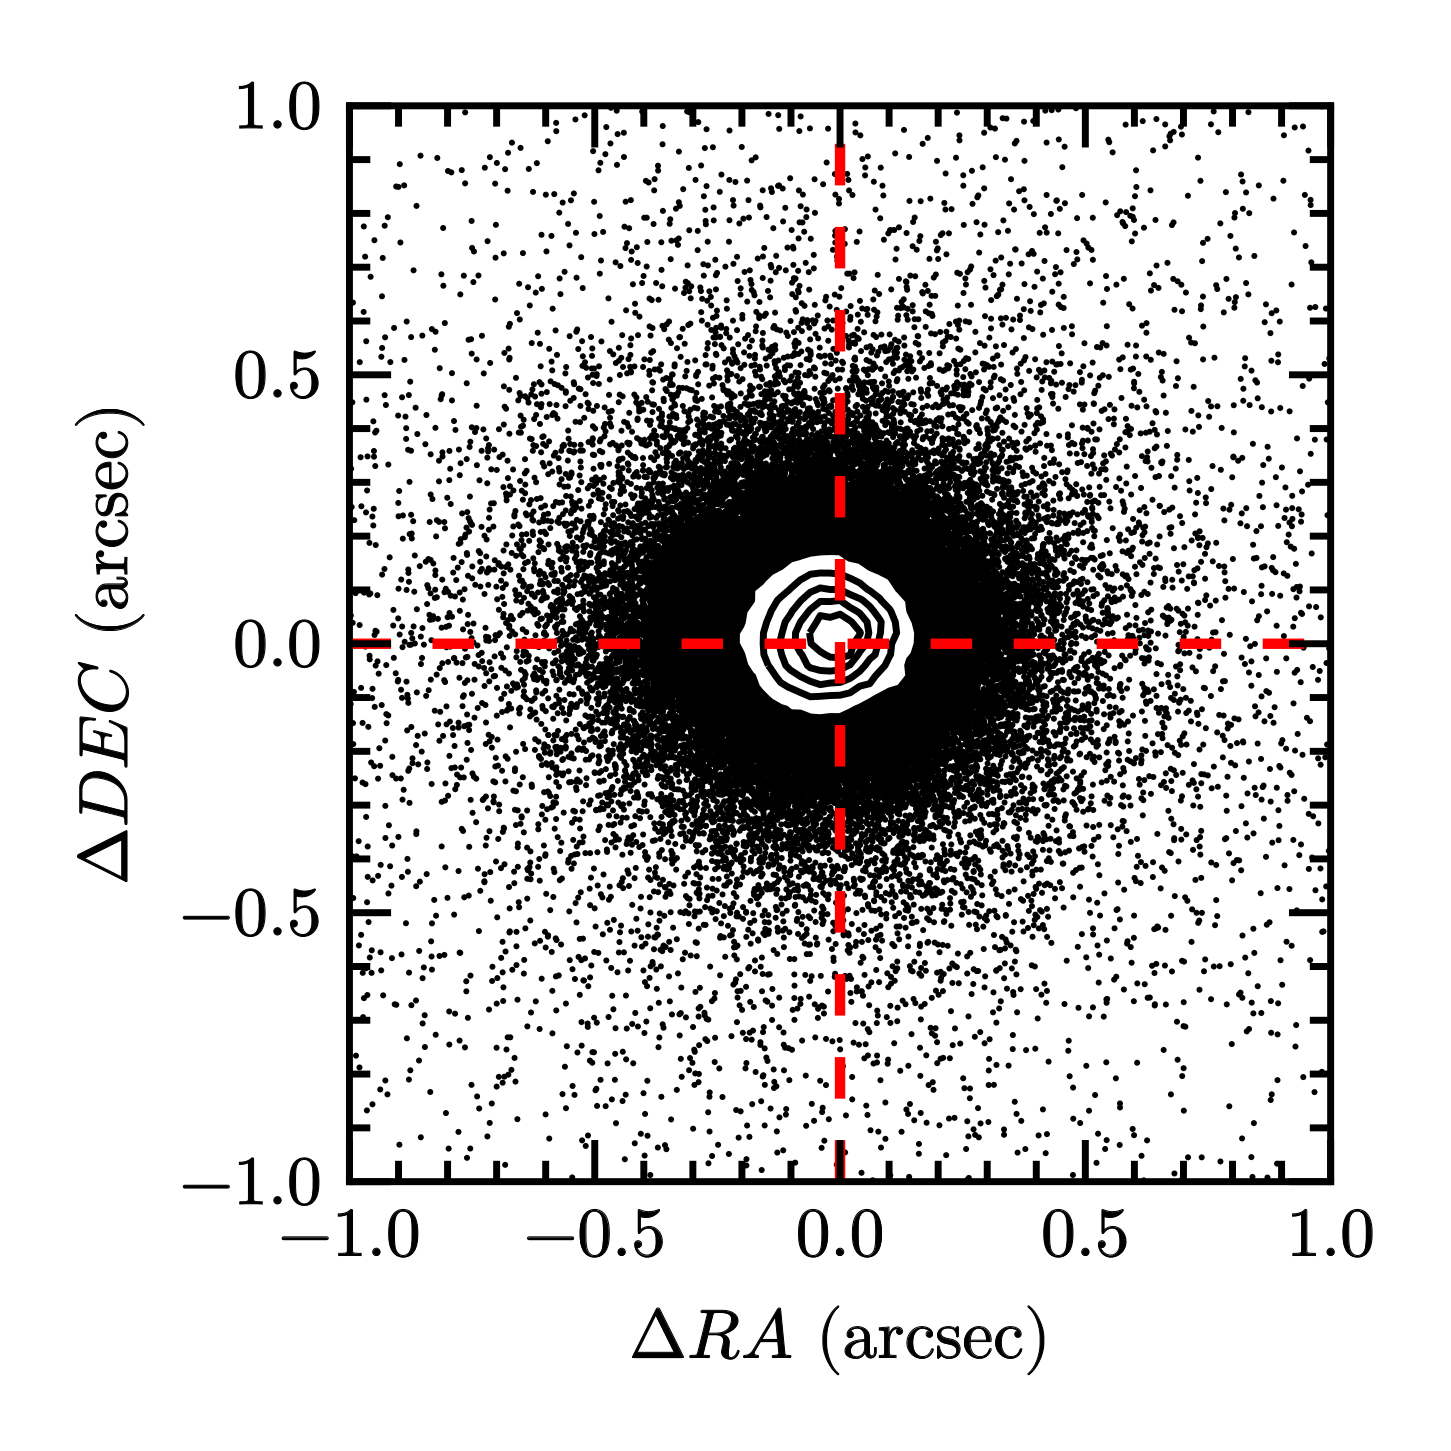
\includegraphics[width=0.5\textwidth]{astrometry_2d_separation.png}}
\subfloat[\label{fig:astrometry_sep}]{
	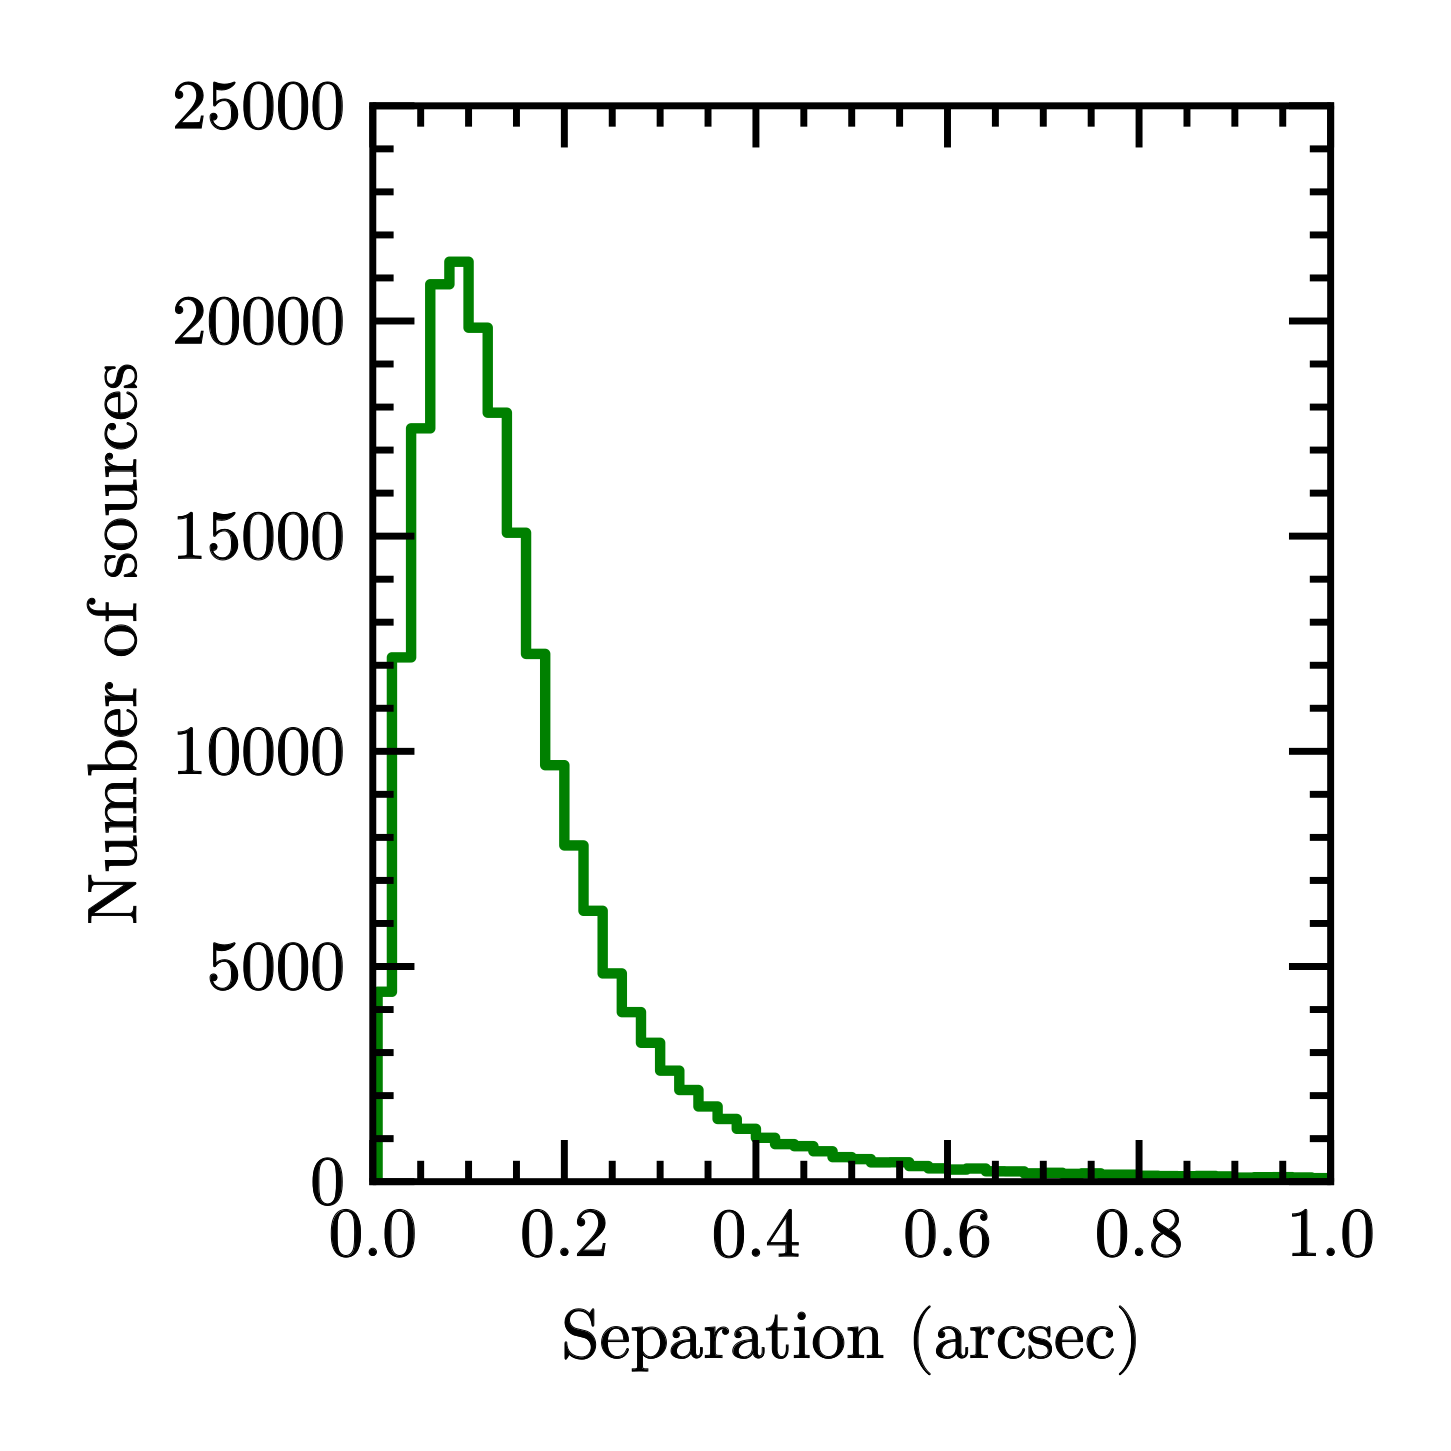
\includegraphics[width=0.5\textwidth]{astrometry_separation.png}}
\caption[Verification of the astrometry]{Comparison between DES and VIDEO astrometry for the \num{199 252} brightest non-duplicate objects, selected by imposing an SLR-corrected magnitude of $z_{\mathrm{DES,AB}}<22.0$. \textbf{(a)} Distribution of the difference  $\Delta RA$ and $\Delta DEC$ between the two surveys as defined in Equations \ref{eqn:ra_offset} and \ref{eqn:dec_offset}. The dashed red lines correspond to an offset of 0. \textbf{(b)} Histogram of the total separation $\Delta=\sqrt{{\Delta RA}^2 + {\Delta DEC}^2}$. Both (a) and (b) indicate excellent astrometric agreement.}
\label{fig:astrometry}
\end{figure*}





\subsection{Photometry verification}
The next validation test compares the photometry between the \DESVIDEO and \cite{2013MNRAS.428.1281J} VIDEO catalogues. For this test, the non-duplicate \DESVIDEO detections were again matched to the \cite{2013MNRAS.428.1281J} objects within a \SI{1}{\arcsec} radius. The magnitude offset between the two surveys was then computed for all matched detections, using magnitudes measured in a $\approx \SI{2}{\arcsec}$ diameter aperture (note: the two catalogues differ slightly in the aperture sizes that have been used  --- \SI{1.95}{\arcsec} for \DESVIDEO and \SI{2}{\arcsec} for \citealt{2013MNRAS.428.1281J}). Figure \ref{fig:mag_comparison} shows the resulting magnitude differences for each VIDEO filter as a function of magnitude. With mean offsets of < \SI{0.022}{\magab} in all filters, the two catalogues are generally in agreement, especially when considering that the \cite{2013MNRAS.428.1281J} apertures are slightly larger.  Despite this broad agreement, one may nevertheless note a slight bias towards bigger mean offsets (i.e. brighter \citealt{2013MNRAS.428.1281J} magnitudes) for redder filters, ranging from 0.007 for the $Z$-band to 0.022 in the $K_{s}$-band. There are several possible explanations for this trend. Firstly, the difference in aperture sizes may play a role. Even though the mean VIDEO PSF actually has a larger FWHM at shorter wavelengths (see Section \ref{subsubsection:data_quality_video}), it is possible that it has more extended wings at longer wavelengths, so that the (smaller) \DESVIDEO aperture catches less of the total flux in the redder filters. Secondly, the \DESVIDEO apertures for a given object have been placed in the same position for all bands (based on the $r+i+z$ detection image), whereas the positions in the \cite{2013MNRAS.428.1281J} catalogues have been derived from the morphology of the object in the reddest detected band (see Section \ref{subsubsection:video_data_reduction}).  For extended sources, this morphology can differ between filters if some regions of a galaxy contain bluer emission than others. Therefore, it is possible that for these sorts of objects the \DESVIDEO apertures are less optimally positioned, so that the \DESVIDEO measurements miss some red flux that is included in the \cite{2013MNRAS.428.1281J} catalogues. Nevertheless, the fact that even in the $K_{s}$-band the mean offsets are no larger than \SI{0.022}{\magab} demonstrates that the general agreement is good. This warrants a good degree of confidence in the accuracy of the \DESVIDEO photometry. \par

% \begin{figure}
% \centering
% \subfloat[\label{}]{
% 	\includegraphics[clip, width=0.50\textwidth]{mag_comparison_Z.png}}
% \subfloat[\label{}]{
% 	\includegraphics[clip, width=0.50\textwidth]{mag_comparison_Y.png}}

% \subfloat[\label{}]{
% 	\includegraphics[clip, width=0.50\textwidth]{mag_comparison_J.png}}
% \subfloat[\label{}]{
% 	\includegraphics[clip, width=0.50\textwidth]{mag_comparison_H.png}}

% \subfloat[\label{}]{
% 	\includegraphics[clip, width=0.50\textwidth]{mag_comparison_K.png}}	

% \caption[Verification of the photometry]{Comparison between VIDEO magnitudes from \DESVIDEO ($m_{\mathrm{DES+VIDEO}}$) and \cite{2013MNRAS.428.1281J} ($m_{\mathrm{VIDEO}}$), for all objects detected in both datasets. The grey dots show the magnitude difference $m_{\mathrm{DES+VIDEO}}-m_{\mathrm{VIDEO}}$ of each source as a function of \DESVIDEO magnitude. The black squares indicate the mean difference in bins of \SI{0.5}{\mag}. The coloured horizontal lines show the total mean value averaged over all grey data points, which is also listed in the legend. It must be noted that \DESVIDEO values have been measured in a \SI{1.95}{\arcsec} diameter aperture, as opposed to \SI{2}{\arcsec} for \cite{2013MNRAS.428.1281J}.}
% \label{fig:mag_comparison}
% \end{figure}

\begin{figure}[ph] 
\centering    
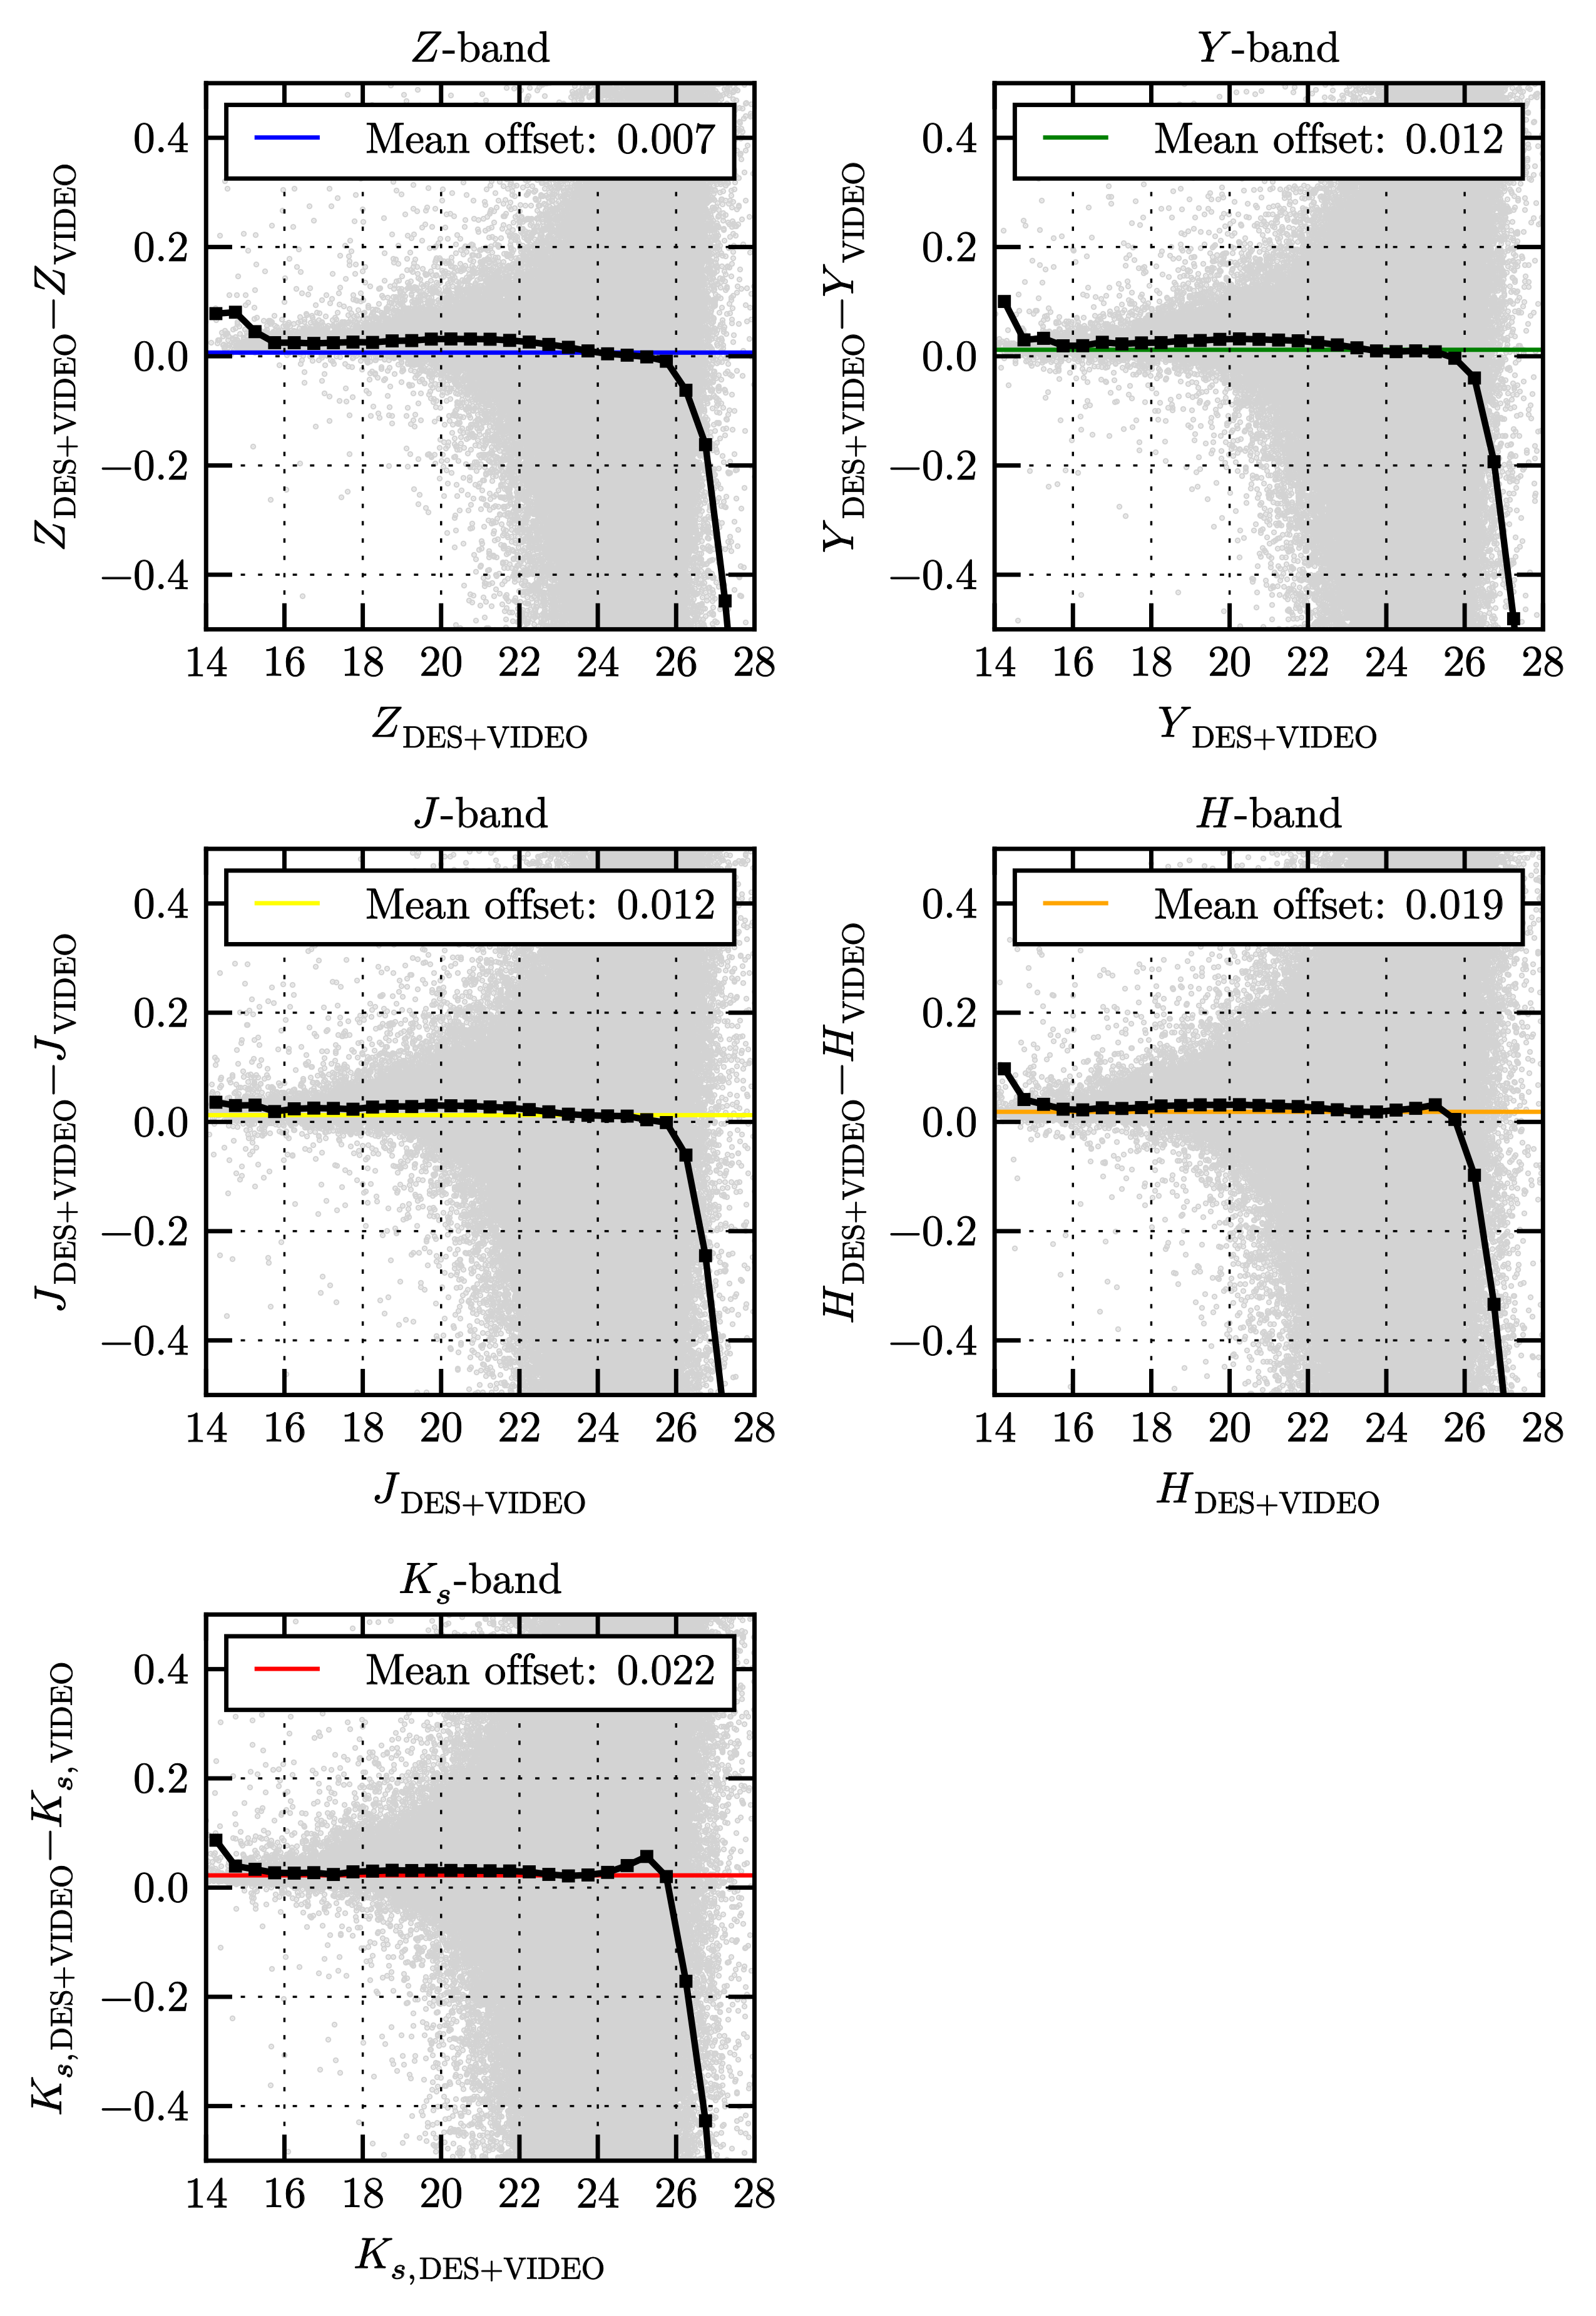
\includegraphics[width=0.95\textwidth]{mag_comparison.png}
\caption[Verification of the photometry]{Comparison between VIDEO magnitudes from \DESVIDEO ($m_{\mathrm{DES+VIDEO}}$) and \cite{2013MNRAS.428.1281J} ($m_{\mathrm{VIDEO}}$), for all objects detected in both datasets. The grey dots show the magnitude difference $m_{\mathrm{DES+VIDEO}}-m_{\mathrm{VIDEO}}$ of each source as a function of \DESVIDEO magnitude. The black squares indicate the mean difference in bins of \SI{0.5}{\mag}. The coloured horizontal lines show the total mean value averaged over all grey data points, which is also listed in the legend. It must be noted that \DESVIDEO values have been measured in a \SI{1.95}{\arcsec} diameter aperture, as opposed to \SI{2}{\arcsec} for \cite{2013MNRAS.428.1281J}.}
\label{fig:mag_comparison}
\end{figure}

 
 
\subsection{Forced photometry verification and results}\label{subsection:forced_phot_verification}
To assess the merits of the \DESVIDEO forced photometry strategy, the current section investigates whether the \DESVIDEO method indeed retrieves measurements for a larger number of sources than  \cite{2013MNRAS.428.1281J}. For this analysis, the \DESVIDEO source counts are compared to the number that would have been obtained via simple catalogue matching between the DESDM and \cite{2013MNRAS.428.1281J} catalogues. In order to estimate the latter number, the author assembled a position-matched dataset via the same catalogue assembly procedure as before (applying step 1, 3, 4, 6, and 8 from the algorithm presented in Section \ref{subsection:catalog_production}), this time using the \cite{2013MNRAS.428.1281J} catalogues instead of \DESVIDEO forced photometry in step 4. Including duplicates\footnote{The new matched catalogue contains duplicates, originating from the same tile overlap pattern that exists in the \DESVIDEO catalogue. A non-duplicate version was also produced.}, position matching retrieved \num{1 862 154} objects, which is 24\% less than the \num{2 443 576} sources obtained before via forced photometry. The unique (i.e. non-duplicate) total equals \num{1 676 054} with the \cite{2013MNRAS.428.1281J} catalogues, a 22\% decrease compared to the \num{2 152 575} unique sources in the forced photometry dataset. These two figures indicate that \DESVIDEO forced photometry indeed significantly increases the amount of information extracted from the VIDEO survey. Even more gains were made in those regions where DES imaging is significantly deeper than VIDEO. For example, in the cdfs1 tile, forced photometry retrieves fluxes for \num{393616} objects (including duplicates), compared to \num{257812} from matching to \cite{2013MNRAS.428.1281J} ---  an improvement of $\approx 35\%$. Without duplicates, these numbers are \num{376079} vs \num{246755}, implying an increase of $\approx 34\%$. \par


\begin{figure*}[tpb]
\centering
\subfloat[\label{fig:number_counts_Ks_total}]{
	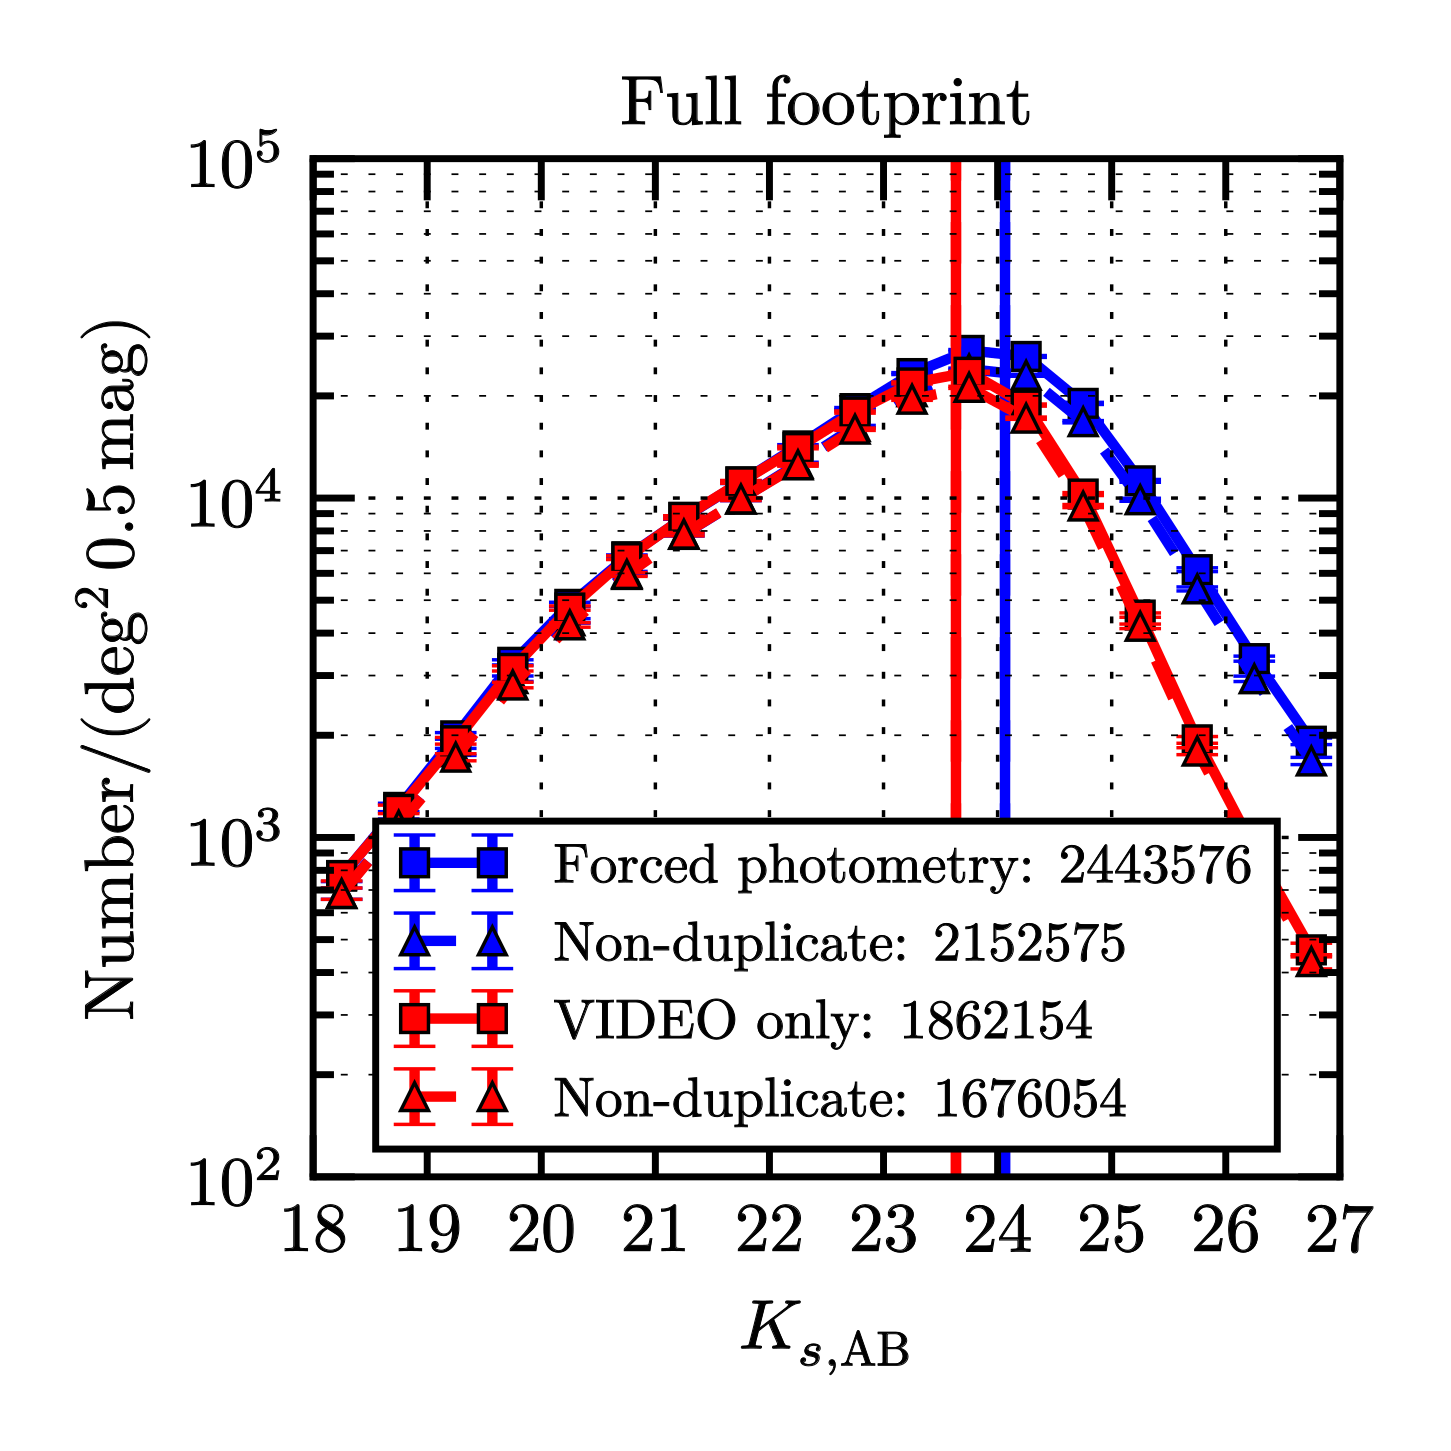
\includegraphics[clip, width=0.50\textwidth]{Chapter2/Figs/number_counts_Ks.png}}
\subfloat[\label{fig:number_counts_Ks_cdfs1}]{
	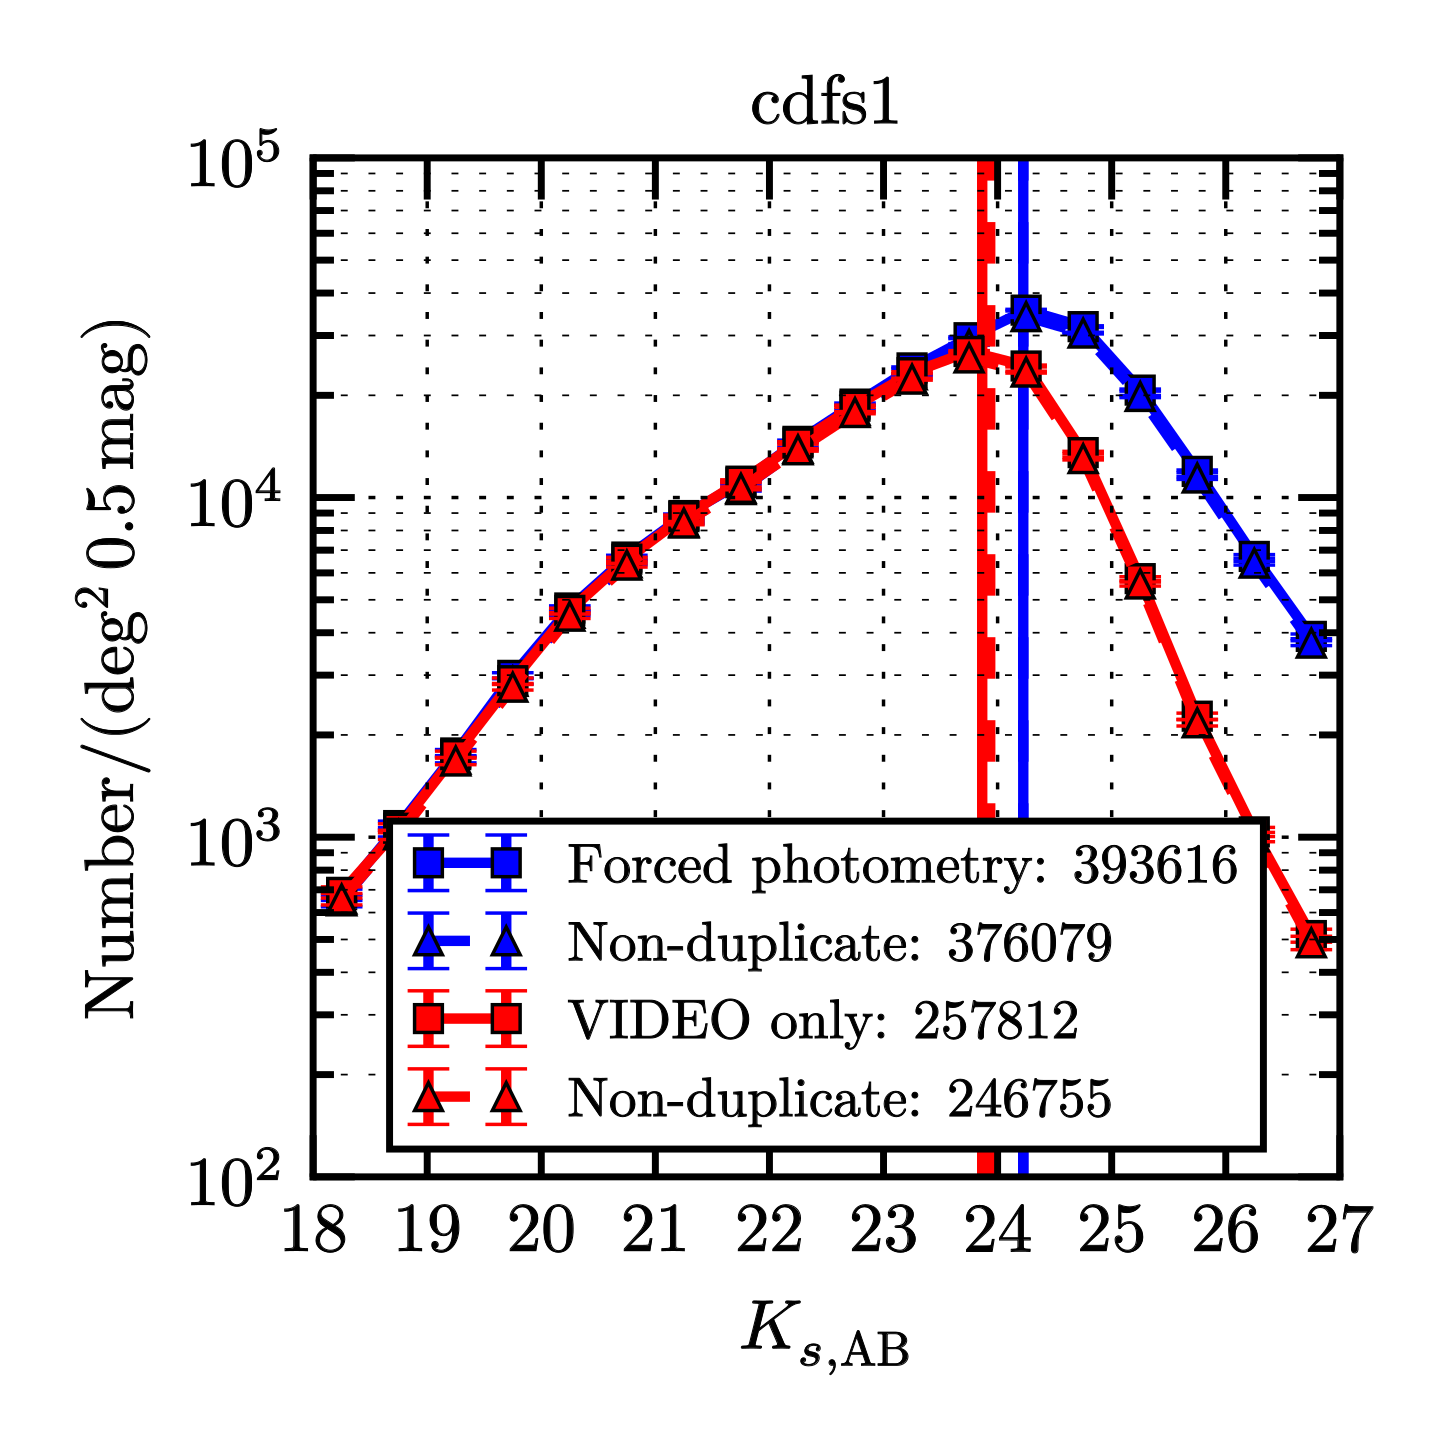
\includegraphics[clip,width=0.50\textwidth]{Chapter2/Figs/number_counts_Ks_cdfs1.png}}
\caption[Number counts in the \texorpdfstring{$K_{s}$}{}-band]{ Number counts per \si{\sqdeg} as a function of $K_{s}$-band magnitude, in bins of \SI{0.5}{\mag}. \DESVIDEO forced photometry (measured in \SI{1.95}{\arcsec} apertures) outcomes are shown in blue. The outcomes from position matching to the \cite{2013MNRAS.428.1281J} VIDEO catalogues (measured in \SI{2}{\arcsec} apertures) are shown in red. Solid lines with squares denote results including duplicates, and the dashed lines and triangles denote results after duplicates have been removed. All data points contain error bars corresponding to Poisson counting uncertainties, but these are smaller than the symbol size in almost all cases. Maxima for all distributions are computed in smaller \SI{0.01}{\mag} bins and denoted by vertical lines. \textbf{(a)} Results for the full \DESVIDEO footprint. The \DESVIDEO maxima both lie at $K_{s,\mathrm{AB}} = 24.065$ (with and without duplicates), and the \cite{2013MNRAS.428.1281J} maxima are at $K_{s,\mathrm{AB}} = 23.635$ (idem). \textbf{(b)} Results for the cdfs1 tile only. The \DESVIDEO maxima lie at $K_{s,\mathrm{AB}} = 24.225$ (with and without duplicates), and the \cite{2013MNRAS.428.1281J} maxima are at $K_{s,\mathrm{AB}} = 23.865$ with duplicates and at $K_{s,\mathrm{AB}} = 23.935$ without duplicates.}
\label{fig:number_counts_Ks}
\end{figure*} 

Further analysis of the number counts also shows that \DESVIDEO forced photometry extracts data for fainter sources than is possible with VIDEO alone. Figure \ref{fig:number_counts_Ks_total}  illustrates this finding by plotting the number of \DESVIDEO vs matched \cite{2013MNRAS.428.1281J} objects as a function of $K_{s}$-band magnitude, per \si{\sqdeg} in bins of \SI{0.5}{\mag}. Like in the previous section, these magnitudes are measured in a $\approx\SI{2}{\arcsec}$ diameter aperture (\SI{1.95}{\arcsec} for \DESVIDEO and \SI{2}{\arcsec} for \citealt{2013MNRAS.428.1281J}). Importantly, the \DESVIDEO number counts agree well with the \cite{2013MNRAS.428.1281J} results at the bright end, but come out considerably higher at the faint end as the \cite{2013MNRAS.428.1281J} distribution starts to roll over. This is exactly the behaviour that one would expect if \DESVIDEO forced photometry indeed extracts data from objects that are too faint to be detected reliably in VIDEO alone. To quantify this increase in faint source counts, the maximum of the $K_{s}$ distribution was determined for both catalogues (grouping magnitudes in smaller bins of \SI{0.01}{\mag} for increased resolution). Without forced photometry, this peak\footnote{All the maxima in this paragraph are given without duplicates, the results including duplicates are shown in Figure \ref{fig:number_counts_Ks} for completeness.} lies at $K_{s,\mathrm{AB}} = 23.635$, whereas the \DESVIDEO peak occurs at $K_{s,\mathrm{AB}} = 24.065$. This indicates that the \DESVIDEO method pushes the VIDEO measurements $\approx \SI{0.4}{\mag}$ fainter (possibly even a bit more given the fact that the \DESVIDEO apertures are slightly smaller than those from \citealt{2013MNRAS.428.1281J}). The above analysis was repeated for the cdfs1 tile studied in the previous paragraph. These results are plotted in Figure \ref{fig:number_counts_Ks_cdfs1}. Here, the \cite{2013MNRAS.428.1281J} maximum occurs at $K_{s,\mathrm{AB}} = 23.935$, while the \DESVIDEO distribution peaks at $K_{s,\mathrm{AB}}=24.225$, i.e. $\approx \SI{0.3}{\mag}$ fainter. This is slightly less than the $\approx \SI{0.4}{\mag}$ increase for the full footprint, most likely due to the fact that the $K_{s}$ data in this tile is slightly deeper than average (see Table \ref{table:error_agreement}). Because \cite{2013MNRAS.428.1281J} based their source detections on the reddest filter in which a given object is detected  (which is often the $K_{s}$-band), in this tile their detection strategy performs slightly above average. Therefore, the  \DESVIDEO forced photometry provides a comparatively smaller increase in faint $K_{s}$-observed sources. One may recall from the previous paragraph that forced photometry does, however, perform above average in the cdfs1 tile in terms of overall source counts (when compared to the full footprint).  This can be attributed to the fact that the $Z$-band imaging is shallower than average in this tile, which means that the corresponding \cite{2013MNRAS.428.1281J} catalogue contains fewer `blue' objects that are undetectable in $YJHK_{s}$ but would nevertheless show up in deeper $Z$-band imaging. At the same time, the DES $z$-band is much deeper than VIDEO in this region, so the \DESVIDEO pipeline does manage to retrieve these blue objects. \par 

The fact that forced photometry can be used to obtain photometry for more and for fainter objects has been shown several times before (e.g. \citealt{2015MNRAS.446.2523B,2016AJ....151...36L,2017ApJS..230....9N}). In fact, the very similar study by \cite{2015MNRAS.446.2523B} demonstrated this principle for the DES wide-field (detection) and VHS (measurement) data. Exploiting the fact that their DES data is considerably deeper than VHS ($\sim\SI{4}{\magab}$ when comparing $i$- and $J$-band magnitudes), they found that forced photometry increases the number of objects with measured VHS fluxes by a factor of 4.5 and pushes the VHS 80\% completeness limit \SI{1.5}{\mag} deeper. Comparatively, the 1.22 times increase in numbers and  \SI{0.4}{\mag} increase in depth found by this thesis are not quite as enormous, since the DES deep field and VIDEO surveys are more evenly matched in terms of limiting magnitudes ($<\SI{2}{\magab}$ difference between $i$ and $J$). However, the \DESVIDEO results nevertheless add to the existing body of evidence in favour of using forced photometry to combine surveys. On top of that, they also demonstrate that doing so can lead to considerable gains even if one survey is only moderately deeper than the other. \par


\begin{figure*}[tpb]
\centering
\subfloat[]{
	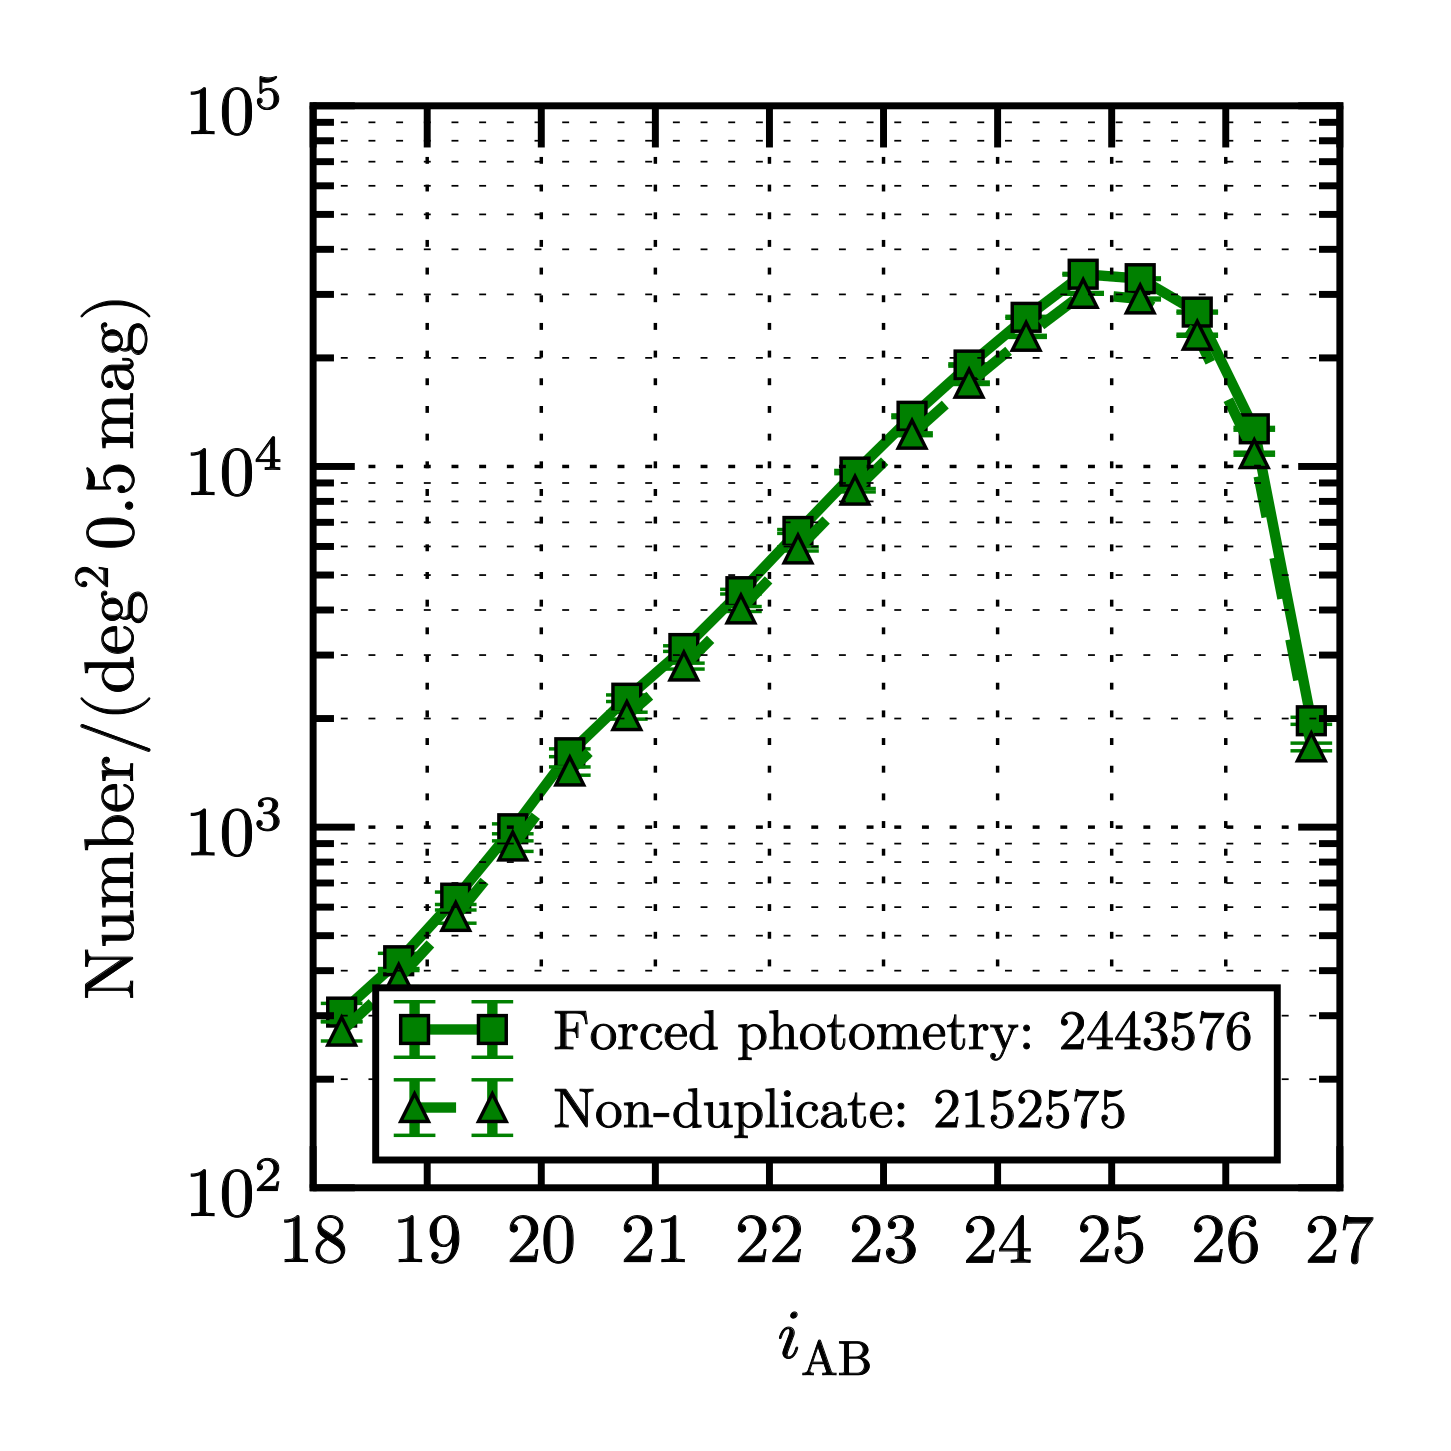
\includegraphics[clip, width=0.50\textwidth]{Chapter2/Figs/number_counts_i.png}}
\subfloat[]{
	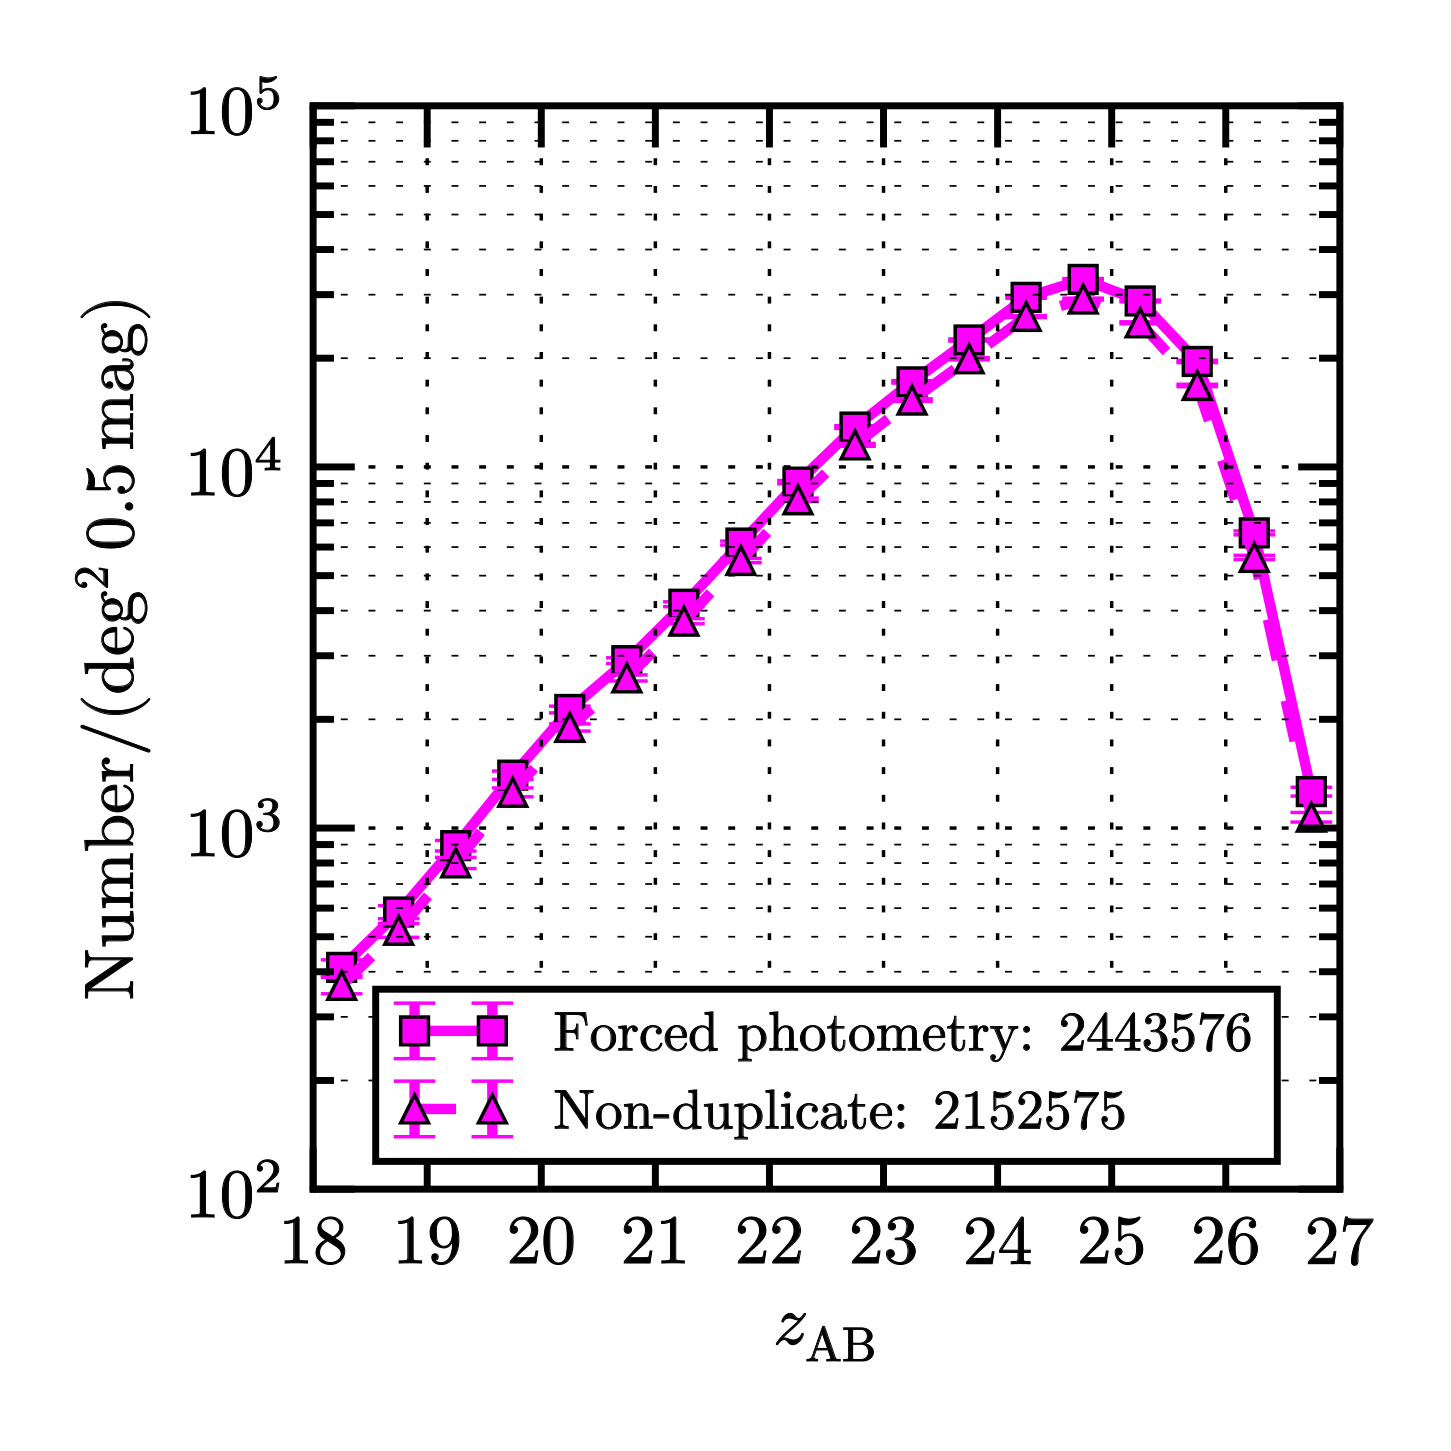
\includegraphics[clip, width=0.50\textwidth]{Chapter2/Figs/number_counts_z.png}}
\caption[Number counts in the \texorpdfstring{$i$}{}-band and \texorpdfstring{$z$}{}-band]{Number counts for the \DESVIDEO catalogue per \si{\sqdeg} as a function of \SI{1.95}{\arcsec} magnitudes in bins of \SI{0.5}{\mag}. The solid lines with squares show results including duplicates, and the dashed lines and triangles show results after duplicates have been removed. Data points for each bin include error bars corresponding to uncertainties from Poisson counting, but these are smaller than the symbol size in almost all cases. \textbf{(a)} Results for the DES $i$-band. \textbf{(b)} Results for the DES $z$-band.}
\label{fig:number_counts_DES}
\end{figure*}


\subsection{Catalogue results}
The validation tests above confirm that the astrometry and photometry of the \DESVIDEO catalogue are indeed accurate, and that the forced photometry is functioning as intended. This establishes the catalogue as a suitable general resource for the scientific community, and demonstrates that it can provide a solid backbone for the photometric redshifts and high-redshift galaxy search later in this thesis. \par 

%The \DESVIDEO catalogue can thus provide a solid backbone for the photometric redshifts and high-redshift galaxy search later in this thesis. 

For the sake of  providing a comprehensive overview of the full catalogue, Figure \ref{fig:number_counts_DES} shows the \DESVIDEO number counts in the $i$-band and $z$-band as a function of magnitude. The distributions behave as expected from the area-depth distributions in Figure \ref{fig:area_depth}. The $z$-band distribution peaks roughly $z_{\mathrm{AB}}\approx24.75$, which approximately corresponds to the $z_{5\sigma}\geq24.9$ magnitude limit for the largest \SI{10.8}{\sqdeg} section of the total footprint. The number counts then decline slightly with increasing magnitude, falling sharply after $z_{\mathrm{AB}}\sim 25.75$. This turning point is reasonably close to the $z_{5\sigma}\geq26.2$ limiting magnitude of the deepest \SI{4.3}{\sqdeg}. Similarly, the maximum of the $i$-band distribution lies around $i_{\mathrm{AB}}\approx25.0$, in agreement with the limiting $i_{5\sigma}\geq25.1$ limiting magnitudes in the largest \SI{10.7}{\sqdeg} $i$-band area. The second turnover at $i_{\mathrm{AB}}\approx 26.0$ again lines up approximately with the $i_{\sigma}\geq26.3$ depths in the deepest \SI{4.4}{\sqdeg} $i$-band regions of the catalogue. \par 
